%--------------------------------------------------------------------
% Vorlage für eine Abschlussarbeit
% Darf ohne Einschränkungen weiterverwendet und abgeändert werden.
% mehr zur Verwedung in der README.md
% ⓒ (CC0) 2016, 2018 Henning Iseke <h_i_@online.de>
%--------------------------------------------------------------------

% Haupdatei

% Befehle für Metadaten
% BUG: bei Verwendung von pdflatex müssen Umlaute ausnahmsweise mit \"u o.ä.
% eingegeben werden, da Paket inputenc noch nicht geladen
% alternativ: verschieben des Blocks in die Präambel
\newcommand*{\titel}{Anwendung von maschinellem Lernen zur Regression am Beispiel des Diphoton-Prozesses}
\newcommand*{\autor}{Andreas Weitzel}
\newcommand*{\geburtsort}{Fulda}
\newcommand*{\geburtsdatum}{10.08.1999}
\newcommand*{\datum}{24.05.2021}
\newcommand*{\institut}{Institut füer Kern- und Teilchenphysik}
\newcommand*{\arbeitsgruppe}{Emmy-Noether-Nachwuchsgruppe}
\newcommand*{\erstgutachter}{Dr. Frank Siegert}
\newcommand*{\zweitgutachter}{Prof. Dr. Arno Streassner}
\newcommand*{\hochschulgrad}{Bachelor of Science}
\newcommand*{\studiengang}{Physik}
\newcommand*{\abschlussarbeit}{Bachelor-Arbeit}
\newcommand*{\schlagworte}{Deep-Learning}


\newcommand{\abstractde}{
Für den Diphoton-Prozess $q\overline{q} \rightarrow \gamma \gamma$ wird der Wirkungsquerschnitt berechnet und auf die hadronische Ebene $pp \rightarrow \gamma \gamma$ übertragen. Anschließend werden Methoden des Deep-Learning verwendet, um die differentiellen Wirkungsquerschnitte zu nähern. Hierbei wird vor allem auf die Schwierigkeit eingegangen, neuronalen Netzen sich um Größenordnungen unterscheidende Labels beizubringen. Weiterhin wird die Eignung und Anwendbarkeit von Transfer-Learning bei Regression von Wirkungsquerschnitten untersucht. Schließlich wird von simplen Monte-Carlo-Methoden Gebrauch gemacht, um die differentiellen Wirkungsquerschnitte zu integrieren. 
}
\newcommand{\abstracten}{
<Abstract english>
}

% comment out the language which you do NOT want
%--------------------------------------------------------------------
% Vorlage für eine Abschlussarbeit
% Darf ohne Einschränkungen weiterverwendet und abgeändert werden.
% mehr zur Verwedung in der README.md
% ⓒ (CC0) 2016, 2018 Henning Iseke <h_i_@online.de>
%--------------------------------------------------------------------

\documentclass[11pt, % 11 Punkt Schriftgröße
german, % standardmäßig deutsche Eigenarten einhalten
abstract=true, % Abstract verwenden
twoside, % Zweiseitig
captions=tableheading, % Tabellenüberschriften mit richtigem Abstand
BCOR=10mm, % TODO: Bindekorrektur, muss je nach Bindung angepasst werden
%draft % TODO: Entwurfsmodus am Ende entfernen
]{scrreprt}

\usepackage{ifluatex} % Paket, um Vorlage für Lua- und pdfLaTeX zu verwenden
\ifluatex % LuaTeX
    %\usepackage{fontspec} % Schriftarten verwalten (es können im Grunde genommen alle installierten Schriftarten verwendet werden)
    %\setmainfont[Ligatures=TeX]{Linux Libertine O} % Hauptschriftart setzen
    %\setsansfont[Ligatures=TeX]{Linux Biolinum O} % Serifenlose Schriftart

    \usepackage{polyglossia} % Namen, Silbentrennung an Sprache anpasen
    \setdefaultlanguage[spelling=new,babelshorthands=true]{german} % Deutsch als Standardsprache
    \setotherlanguage{english} % weitere Sprache (für Abstract)

    \newcommand*{\compiler}{Lua\LaTeX}
\else % kein LuaTeX
    \usepackage[utf8]{inputenc} % Kodierung der Datei
    \usepackage[T1]{fontenc} % Vollen Umfang der Schriftzeichen
    \usepackage[main=ngerman,english]{babel} % Sprache auf Deutsch (neue Rechtschreibung)
    \newenvironment{english}{\begin{otherlanguage}{english}}{\end{otherlanguage}}
    \newcommand*{\compiler}{pdf\LaTeX}
    %\usepackage{libertine} % Schriftart Linux Libertine/Biolinum verwenden
\fi

\usepackage{siunitx} % Darstellung von Größen
\sisetup{locale=DE, % in Deutschland übliche Darstellung
separate-uncertainty, % Unsicherheit mit ± getrennt darstellen
table-number-alignment=center, % Zahlen in Tabellen zentrieren (mit Option S)
}

\usepackage{graphicx} % Einbinden von Grafiken
\usepackage{pdfpages} % Einbinden von PDF-Grafiken

\usepackage{booktabs} % schöne Tabellen mit \toprule, \midrule, \bottomrule
\usepackage{multirow}
\usepackage{multirow} % mehrzeilige Zellen
\usepackage{csquotes} % Anführungszeichen mit \enquote
\usepackage[automark]{scrlayer-scrpage} % Seiten mit Kopf- und Fußzeile gestalten
\pagestyle{scrheadings} % Seitenstil setzen
%\usepackage{microtype} % Mikrotypographie

% Literaturangaben
\usepackage[backend=biber, % Biber zum Erstellen verwenden: biber <Dokument>
style=phys, % in der Physik üblichen Stil
articletitle=false, % ohne Titel bei Artikeln (bei Büchern, … schon)
pageranges=false, % nur Anfangsseitenzahl
language=german, % deutsche Sprache
biblabel=brackets % Verweise als „[1]“
]{biblatex} % Literaturverzeichnis
\addbibresource{literatur} % bib-Datei mit den Infos zur Literatur
%\renewcommand*{\bibfont}{\small} % kleine Schriftart für Literaturverzeichnis

% Mathematik
\usepackage{amsmath} % Umgebungen/Befehle, die für Mathe nützlich sind
\usepackage{amssymb}
\ifluatex
\usepackage{unicode-math} % Symbole für Mathematik
%\setmathfont{Asana-Math.otf} % Schriftart für den Mathemodus (nur mit LuaLaTeX)
\fi
\usepackage{physics} % Umgebungen/Befehle für Physik
\usepackage{cancel}

\usepackage{caption} % Anpassung der Bildunterschriften, Tabellenüberschriften
\usepackage{subcaption} % mehrere Unterabbilungen in einer Abbildung, auch Tabellen

\usepackage[hidelinks,pdfauthor={\autor},
pdfsubject=Abschlussarbeit,pdftitle={\titel},pdfkeywords={\schlagworte}
unicode=true]{hyperref} % Metadaten und Links in PDFs

% Nummerierung anpassen
\numberwithin{equation}{chapter}
\numberwithin{figure}{chapter}
\numberwithin{table}{chapter}


%%--------------------------------------------------------------------
% Vorlage für eine Abschlussarbeit
% Darf ohne Einschränkungen weiterverwendet und abgeändert werden.
% mehr zur Verwedung in der README.md
% ⓒ (CC0) 2016, 2018 Henning Iseke <h_i_@online.de>
%--------------------------------------------------------------------

\documentclass[11pt, % 11 Punkt Schriftgröße
german, % standardmäßig deutsche Eigenarten einhalten
abstract=true, % Abstract verwenden
twoside, % Zweiseitig
captions=tableheading, % Tabellenüberschriften mit richtigem Abstand
BCOR=10mm, % TODO: Bindekorrektur, muss je nach Bindung angepasst werden
%draft % TODO: Entwurfsmodus am Ende entfernen
]{scrreprt}

\usepackage{ifluatex} % Paket, um Vorlage für Lua- und pdfLaTeX zu verwenden
\ifluatex % LuaTeX
    %\usepackage{fontspec} % Schriftarten verwalten (es können im Grunde genommen alle installierten Schriftarten verwendet werden)
    %\setmainfont[Ligatures=TeX]{Linux Libertine O} % Hauptschriftart setzen
    %\setsansfont[Ligatures=TeX]{Linux Biolinum O} % Serifenlose Schriftart

    \usepackage{polyglossia} % Namen, Silbentrennung an Sprache anpasen
    \setdefaultlanguage{english} % English as default language
    \setotherlanguage{german} % weitere Sprache (für Abstract)

    \newcommand*{\compiler}{Lua\LaTeX}
\else % kein LuaTeX
    \usepackage[utf8]{inputenc} % Kodierung der Datei
    \usepackage[T1]{fontenc} % Vollen Umfang der Schriftzeichen
    \usepackage[main=english, ngerman]{babel} % Sprache auf Deutsch (neue Rechtschreibung)
    \newenvironment{german}{\begin{otherlanguage}{german}}{\end{otherlanguage}}
    \newcommand*{\compiler}{pdf\LaTeX}
    %\usepackage{libertine} % Schriftart Linux Libertine/Biolinum verwenden
\fi

\usepackage{siunitx} % Darstellung von Größen
\sisetup{locale=UK, % in United Kingdom usual setting
separate-uncertainty, % Unsicherheit mit ± getrennt darstellen
table-number-alignment=center, % Zahlen in Tabellen zentrieren (mit Option S)
}

\usepackage{graphicx} % Einbinden von Grafiken

\usepackage{booktabs} % schöne Tabellen mit \toprule, \midrule, \bottomrule
\usepackage{multirow} % mehrzeilige Zellen
\usepackage{csquotes} % Anführungszeichen mit \enquote
\usepackage[automark]{scrpage2} % Seiten mit Kopf- und Fußzeile gestalten
\pagestyle{scrheadings} % Seitenstil setzen
%\usepackage{microtype} % Mikrotypographie

% Literaturangaben
\usepackage[backend=biber, % Biber zum Erstellen verwenden: biber <Dokument>
style=phys, % in der Physik üblichen Stil
articletitle=false, % ohne Titel bei Artikeln
pageranges=false, % nur Anfangsseitenzahl
language=english, % English language
biblabel=brackets % Verweise als „[1]“
]{biblatex} % Literaturverzeichnis
\addbibresource{literatur} % bib-Datei mit den Infos zur Literatur
%\renewcommand*{\bibfont}{\small} % kleine Schriftart für Literaturverzeichnis

% Mathematik
\usepackage{amsmath} % Umgebungen/Befehle, die für Mathe nützlich sind
\ifluatex
\usepackage{unicode-math} % Symbole für Mathematik
%\setmathfont{Asana-Math.otf} % Schriftart für den Mathemodus (nur mit LuaLaTeX)
\fi
\usepackage{physics} % Umgebungen/Befehle für Physik

\usepackage{caption} % Anpassung der Bildunterschriften, Tabellenüberschriften
\usepackage{subcaption} % mehrere Unterabbilungen in einer Abbildung, auch Tabellen

\usepackage[hidelinks,pdfauthor={\autor},
pdfsubject=Thesis,pdftitle={\titel},pdfkeywords={\schlagworte},
unicode=true]{hyperref} % Metadaten und Links in PDFs

% Nummerierung anpassen
\numberwithin{equation}{chapter}
\numberwithin{figure}{chapter}
\numberwithin{table}{chapter}


%\input{befehle}
\captionsetup{format=plain}
\addto\captionsngerman{\renewcommand{\figurename}{Abb.}}

\begin{document}
% Abschnitte
%--------------------------------------------------------------------
% Vorlage für eine Abschlussarbeit
% Darf ohne Einschränkungen weiterverwendet und abgeändert werden.
% mehr zur Verwedung in der README.md
% ⓒ (CC0) 2016, 2018 Henning Iseke <h_i_@online.de>
%--------------------------------------------------------------------

\pagenumbering{roman}
% „Cover“ – kommt für den Druck evtl. in externes Dokument
%\includepdf{bilder/Titelseite}

\titlehead{{\Large

\includegraphics[height=1cm]{graphics/TU_Dresden_Logo}\\[3ex]
Technische Universität Dresden \hfill }\\
Bereich Mathematik und Naturwissenschaften\\
Fakultät Physik\\[1ex]
\institut{}\\
\arbeitsgruppe{}}
\subject{\abschlussarbeit{}\\\textnormal{zur Erlangung des Hochschulgrades}\\
\hochschulgrad{} \\ \textnormal{im Studiengang} \\ \studiengang{}}
\title{\titel}
\subtitle{}
\author{vorgelegt von\\\autor{}\\geboren am \geburtsdatum{} in \geburtsort{}}
\date{eingereicht am \datum{}}
\publishers{}
\lowertitleback{\begin{tabular}{ll}
Erstgutachter: & \erstgutachter{}\\
Zweitgutachter: & \zweitgutachter{}\end{tabular}}
\uppertitleback{\tiny Dokument erstellt mit \compiler{}.}
\maketitle

\begin{minipage}{.95\textwidth}
\begin{abstract}
\abstractde
\end{abstract}
\end{minipage}

\begin{english}
\begin{minipage}{.95\textwidth}
\begin{abstract}
\abstracten
\end{abstract}
\end{minipage}
\end{english}

\cleardoublepage
\tableofcontents
\cleardoublepage
\pagenumbering{arabic}

%%--------------------------------------------------------------------
% Vorlage für eine Abschlussarbeit
% Darf ohne Einschränkungen weiterverwendet und abgeändert werden.
% mehr zur Verwedung in der README.md
% ⓒ (CC0) 2016, 2018 Henning Iseke <h_i_@online.de>
%--------------------------------------------------------------------

\pagenumbering{roman}
% „Cover“ – kommt für den Druck evtl. in externes Dokument
%\includepdf{bilder/Titelseite}

\titlehead{{\Large

\includegraphics[height=1cm]{graphics/TU_Dresden_Logo}\\[3ex]
Technische Universität Dresden \hfill }\\
Bereich Mathematik und Naturwissenschaften\\
Fakultät Physik\\[1ex]
\institut{}\\
\arbeitsgruppe{}}
\subject{\abschlussarbeit{}\\\textnormal{zur Erlangung des Hochschulgrades}\\
\hochschulgrad{} \\ \textnormal{im Studiengang} \\ \studiengang{}}
\title{\titel}
\subtitle{}
\author{vorgelegt von\\\autor{}\\geboren am \geburtsdatum{} in \geburtsort{}}
\date{eingereicht am \datum{}}
\publishers{}
\lowertitleback{\begin{tabular}{ll}
Erstgutachter: & \erstgutachter{}\\
Zweitgutachter: & \zweitgutachter{}\end{tabular}}
\uppertitleback{\tiny Document created with \compiler{}.}
\maketitle

\begin{minipage}{.95\textwidth}
\begin{abstract}
\abstracten
\end{abstract}
\end{minipage}

\begin{german}
\begin{minipage}{.95\textwidth}
\begin{abstract}
\abstractde
\end{abstract}
\end{minipage}
\end{german}

\cleardoublepage
\tableofcontents
\cleardoublepage
\pagenumbering{arabic}

%\include{chapters/einleitung}
% TODO LHAPDF reinschreiben, dass du da dieses Modul benutzt hast
\chapter{Einleitung}
Maschinelles Lernen (ML) ist ein Schlagwort und Konzept, das zwar schon lange in Umlauf ist, jedoch neuerdings extrem an Beliebtheit gewonnen hat. Auch in der Physik haben verschiedene Methoden bereits Einzug gehalten, wobei verschiedene Arten des maschinellen Lernens für unterschiedliche Anwendungsmöglichkeiten verwendet werden. Besonders beliebt ist Deep-Learning, das einen Bereich des maschinellen Lernens bezeichnet, in dem tiefe neuronale Netze verwendet werden. In dieser Arbeit soll die Eignung neuronaler Netzen zur Regression von differentiellen Wirkungsquerschnitten untersucht werden. Dies wird am Beispiel des Diphoton-Prozess angewendet, den wir sowohl auf partonischer Ebene, als auch auf hadronischer Ebene in führender Ordnung analytisch herleiten werden.\\
\newline
Wir beginnen in \textit{\autoref{2}} mit der theoretischen Behandlung des Diphoton-Prozesses im Rahmen der Quantenelektrodynamik und leiten analytisch Ausdrücke für den differentiellen Wirkungsquerschnitt für den Prozess auf partonischer und hadronischer Ebene her. \textit{\autoref{3}} beschäftigt sich zunächst mit den Konzepten hinter Maschinellem Lernen und speziell Deep-Learning mit tiefen neuronalen Netzen (DNN). Am Ende des Kapitels gehen wir noch kurz auf die Grundlagen von einer simplen Monte-Carlo-Integration (MC-Integration) ein. Die Anwendung der DNN folgt in \textit{\autoref{4}}, wobei wir zunächst die differentiellen Wirkungsquerschnitte des Diphoton-Prozesses nähern. Anschließend untersuchen wir das Lernen von Reweights zwischen Fits von Partondichtefunktionen (PDF) und die Eignung von Transfer-Learning (TL) zur Anpassung von einem bereits bestehenden Modell an ein neues PDF-Set. \\
\newline
In dieser Arbeit werden gegebenfalls Abkürzungen verwendet, die bei Bedarf hier \textit{\autoref{label}} nachgelesen werden können. \\
Wir verwenden durchweg natürliche Einheiten, sprich $\hbar = \epsilon_0 = 1$. Vektoren werden mit Fett gedruckten Kleinbuchstaben (Bsp. $\mathbf{x}$) und Matrizen oder Tensoren mit Fett gedruckten Großbuchstaben (Bsp. $\mathbf{M}$) notiert. Speziell Dreiervektoren werden mit einem Pfeil gekennzeichnet (Bsp. $\vec{p}$). Vierervektoren ergeben sich aus dem Kontext. \\
\newline
Der gesamte Python-Code, der während dieser Arbeit verwendet wurde, kann unter https://github.com/andiw99/Bachelor-Thesis eingesehen werden. Hierbei sind alle Skripte zur Generation der Diagramme im Ordner \glqq Plotscripts\grqq~durchnummeriert zu finden. Alle mit ML in Verbindung stehenden Funktionen und Klassen sind in ml.py definiert. Analoges gilt für MC.py. Wir nutzen TensorFlow 2.4.1, wobei die Skripte auch mit TensorFlow 2.... getestet wurden.

\chapter{Diphoton-Prozess}
\label{2}
\section{Partonischer Diphoton-Prozess}
\begin{wrapfigure}{r}{0.7\textwidth}
	\subfloat[t-Kanal]{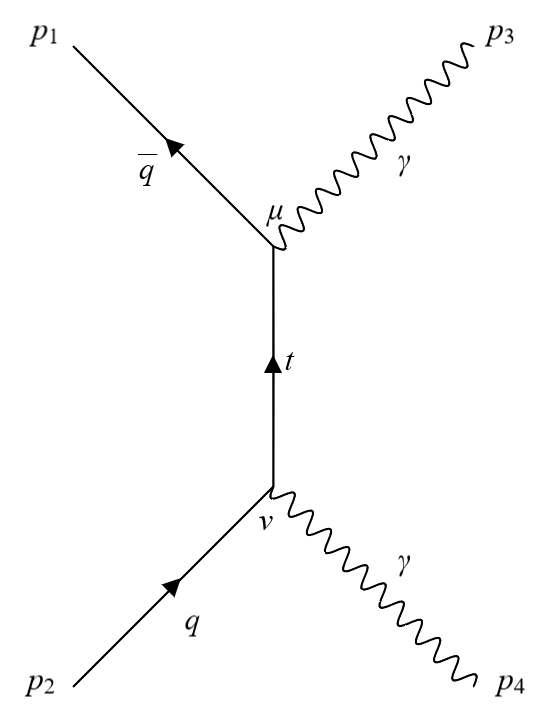
\includegraphics[width=45mm]{graphics/t.png}}
	\subfloat[u-Kanal]{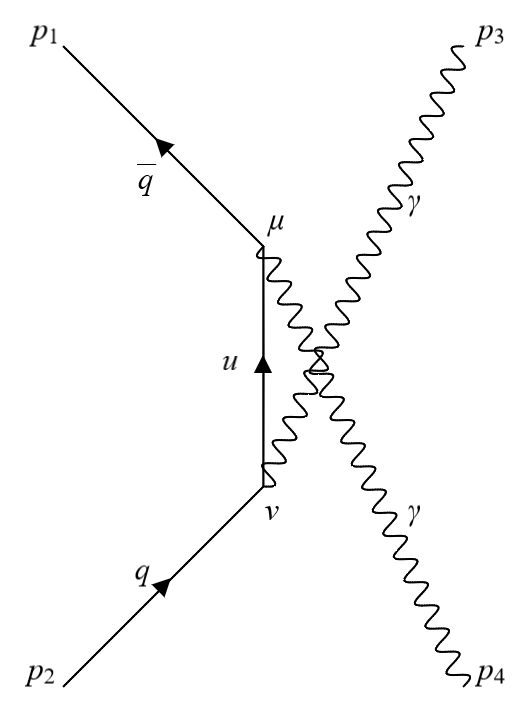
\includegraphics[width=45mm]{graphics/u.png}}
	\caption{Feynman-Diagramme des Diphoton-Prozesses führender Ordnung}
\end{wrapfigure}
Im folgenden wir der Diphoton-Prozess auf partonischer Ebene behandelt.

 Explizit bedeutet dies die Interaktion $q\overline{q} \rightarrow \gamma \gamma$. Unser Ziel ist die Bestimmung der differentiellen Wirkungsquerschnitte, die wir über Fermis goldene Regel berechnen wollen. Dazu benötigen wir die lorenz-invarianten Matrixübergangselemente der grundlegenden Reaktion. Das heißt wir erstellen zunächst alle möglichen Feynman-Diagramme und ein Diagramm, das die Kinematik des Prozesses zeigt.\\
Die Feynman-Regeln der QED liefern dann die folgenden Beiträge der Kanäle:
t-Kanal:
\begin{equation}
 \mathcal{M}_t = \overline{\nu}\left(p_1\right) \left(-iQ_qe\gamma^\mu\right) \epsilon^*_\mu\left(p_3\right) \left(\frac{\gamma^\mu \left(p_{1,\mu} - p_{3, \mu}\right)}{\left(p_1 - p_3\right)^2}\right) \left(-iQ_qe\gamma^\nu\right) \epsilon^*_\nu\left(p_4\right) u\left( p_2\right)
 \label{Gleichung1_1}
\end{equation}
u-Kanal:
\begin{equation}
	 \mathcal{M}_u = \overline{\nu}\left(p_1\right) \left(-iQ_qe\gamma^\mu\right) \epsilon^*_\mu\left(p_4\right) \left(\frac{\gamma^\mu \left(p_{1,\mu} - p_{4, \mu}\right)}{\left(p_1 - p_4\right)^2}\right) \left(-iQ_qe\gamma^\nu\right) \epsilon^*_\nu\left(p_3\right) u\left( p_2\right)
	 \label{Gleichung1_2}
\end{equation}

Dabei wurden die Massen der Quarks vernachlässigt.

Wir nutzen die Notation $\gamma^\mu p_\mu = \cancel{p}$ und die Mandelstam-Variablen  und vereinfachen damit die Ausdrücke \autoref{Gleichung1_1} und \autoref{Gleichung1_2} zu:

\begin{equation}
\mathcal{M}_t = -\frac{Q_q^2e^2}{t}\left[ \overline{\nu}(p_1) \gamma^\mu \epsilon^*_\mu(p_3) \left(\cancel{p}_1 - \cancel{p}_3\right) \gamma^\nu \epsilon^*_\nu(p_4) u(p_2)\right] 
\end{equation}

\begin{equation}
	\mathcal{M}_u = -\frac{Q_q^2e^2}{u}\left[ \overline{\nu}(p_1) \gamma^\mu \epsilon^*_\mu(p_4) \left(\cancel{p}_1 - \cancel{p}_4\right) \gamma^\nu \epsilon^*_\nu(p_3) u(p_2)\right]
\end{equation}
Explizites Einsetzen der Vierervektoren aus der kinematischen Skizze im Schwerpunktsystem, in dem beide einlaufenden Quarks jeweils einen Impuls $p$ besitzen, führt auf:

\begin{equation}
	t = \left(p_1 -p_3\right)^2 = -4 p^2 \cos^2\left(\frac{\theta}{2}\right) \quad \text{und} \quad u = (p_1-p_4)^2 = -4p^2 \sin^2\left(\frac{\theta}{2}\right)
\end{equation} 

Wir können nun das gesamt Matrixelement berechnen, indem wir die Anteile des u- und t-Kanals summieren:
\begin{equation}
	\begin{aligned}
	     \mathcal{M} = \mathcal{M}_u + \mathcal{M}_t &= \mathcal{F} \left[\overline{\nu}(p_1) \left(\frac{\Gamma_t}{\cos^2\left(\frac{\theta}{2}\right)}  +
	     \frac{\Gamma_u}{\sin^2\left(\frac{\theta}{2}\right)} \right) u(p_2) \right] \\
	     &= \mathcal{F} \left[ \overline{\nu}(p_1) \Gamma u(p_2)\right]
	\end{aligned}
\end{equation}
Wobei wir die Ersetzungen \autoref{label} gewählt haben.
\begin{equation}
	\begin{split}
		\Gamma_t = \gamma^\mu \epsilon^*_\mu(p_3) (\cancel{p}_1- \cancel{p}_3)  \gamma^\nu \epsilon_\nu^*(p_4) \quad &\text{und} \quad \Gamma_u = \gamma^\mu \epsilon^*_\mu(p_4) (\cancel{p}_1- \cancel{p}_4)  \gamma^\nu \epsilon_\nu^*(p_3) \\
		\text{sowie} \quad \mathcal{F} = \frac{Q_q^2e^2}{4p^2} \quad &\text{und} \quad \Gamma = \frac{\Gamma_t}{\cos^2\left(\frac{\theta}{2}\right)}  +
		\frac{\Gamma_u}{\sin^2\left(\frac{\theta}{2}\right)} \\
		\cos^2\left(\frac{\theta}{2}\right) = a \quad &\text{und} \quad \sin^2\left(\frac{\theta}{2}\right) = b
	\end{split}
\end{equation}
Um das gemittelte Quadrat des Betrags nun zu berechnen, müssen wir Polarisation und Helizität der Photonen summieren, sowie durch die Anzahl der Anfangszustände der eingehenden Quarks teilen. Die Quarks können drei verschiedene Farbzustände und jeweils zwei verschiedene Helizitäten annehmen. Insgesamt liefern die Anfangszustände also einen Faktor $1/12$:
\begin{equation}
	\left\langle  \abs{\mathcal{M}}^2\right\rangle = \frac{1}{12} \sum_{Hel.} \sum_{Pol.} \abs{\mathcal{M}}^2
\end{equation}
Um die Summe über die Helizitäten auszuführen, verwenden wir Casimirs Trick:
\begin{equation}
	\sum_{Hel.} \abs{\mathcal{M}}^2 = \mathcal{F}^2 \sum_{Hel.}  \left[ \overline{\nu}(p_1) \Gamma u(p_2)\right] \left[\overline{\nu}(p_1) \Gamma u(p_2)\right]^* = \mathcal{F}^2~\text{Tr}\left[ \Gamma \cancel{p}_2 \overline{\Gamma} \cancel{p}_1 \right]
\end{equation}
Wobei $\overline{\Gamma} = \gamma^0\Gamma^\dagger\gamma^0 = \frac{\overline{\Gamma}_t}{a} + \frac{\overline{\Gamma}_u}{b}$ die Dirac-Adjungierte bezeichnet. Für die Dirac-adjungierten $\overline{\Gamma}_t, \overline{\Gamma}_u$ ergibt sich:
\begin{equation}
			\overline{\Gamma}_t = \gamma^\nu \epsilon_\nu(p_4) (\cancel{p}_1- \cancel{p}_3)  \gamma^\mu \epsilon_\mu(p_3) \quad \text{und} \quad \overline{\Gamma}_u = \gamma^\nu \epsilon_\nu(p_3) (\cancel{p}_1- \cancel{p}_4)  \gamma^\mu \epsilon_\mu(p_4)
\end{equation}
\autoref{label} wird damit zu:
\begin{equation}
	\mathcal{F}^2~\text{Tr}\left[ \Gamma \cancel{p}_2 \overline{\Gamma} \cancel{p}_1 \right] = \mathcal{F}^2~\text{Tr}\left[\frac{1}{a^2} \Gamma_t \cancel{p}_2 \overline{\Gamma}_t \cancel{p}_1 + \frac{1}{ab} \Gamma_t \cancel{p}_2 \overline{\Gamma}_u \cancel{p}_1 + \frac{1}{ba} \Gamma_u \cancel{p}_2 \overline{\Gamma}_t \cancel{p}_1 + \frac{1}{b^2} \Gamma_u \cancel{p}_2 \overline{\Gamma}_u \cancel{p}_1\right]
\end{equation}
Wobei wir die Terme von links nach rechts nach folgendem Schema benennen:
\begin{equation}
	T_{ij} = \mathcal{F}^2~\text{Tr}\left[ \frac{1}{ij} \Gamma\left(i\right) \cancel{p}_2 \overline{\Gamma}\left(j\right) \cancel{p}_1 \right] \quad \text{mit} \quad i,j \in \left\lbrace a,b\right\rbrace
\end{equation}
Wir evaluieren nun diese Terme. Wir beginnen mit den Fällen $i = j$:
\begin{equation}
	\begin{aligned}
	T_{aa} &= \frac{1}{a^2}~\text{Tr}\left[ \gamma^\mu \epsilon^*_\mu(p_3) (\cancel{p}_1- \cancel{p}_3)  \gamma^\nu \epsilon_\nu^*(p_4) \cancel{p}_2 \gamma^\nu \epsilon_\nu(p_4) (\cancel{p}_1- \cancel{p}_3)  \gamma^\mu \epsilon_\mu(p_3) \cancel{p}_1 \right] \\
	&=\frac{1}{a^2} \epsilon^*_\mu(p_3)\epsilon_\mu(p_3)\epsilon_\nu^*(p_4)\epsilon_\nu(p_4) ~\text{Tr}\left[-2\gamma^\mu(\cancel{p}_1- \cancel{p}_3) \cancel{p}_2 (\cancel{p}_1- \cancel{p}_3)\gamma^\mu \cancel{p}_1\right] \\
	&=\frac{4\epsilon}{a^2}~\text{Tr}\left[(\cancel{p}_1- \cancel{p}_3) \cancel{p}_2 (\cancel{p}_1- \cancel{p}_3)\cancel{p}_1\right] \\
	&=\frac{32\epsilon}{a^2}(p_3\cdot p_2)(p_3\cdot p_1)
	\end{aligned}
\end{equation}
Wobei die Abkürzung $\epsilon = \epsilon^*_\mu(p_3)\epsilon_\mu(p_3)\epsilon_\nu^*(p_4)\epsilon_\nu(p_4)$ verwendet wurde. Es folgt analog:
\begin{equation}
	T_{bb} = \frac{32\epsilon}{b^2}(p_4\cdot p_2)(p_4\cdot p_1)
\end{equation}
Für $i \neq j$ ergibt sich:
\begin{equation}
	\begin{aligned}
	T_{ab} &= \frac{1}{ab}~\text{Tr}\left[\gamma^\mu \epsilon^*_\mu(p_4) (\cancel{p}_1- \cancel{p}_4)  \gamma^\nu \epsilon_\nu^*(p_3) \cancel{p}_2 \gamma^\nu \epsilon_\nu(p_4) (\cancel{p}_1- \cancel{p}_3)  \gamma^\mu \epsilon_\mu(p_3) \cancel{p}_1 \right] \\
	&=\frac{\epsilon}{ab}~\text{Tr}\left[\gamma^\mu (\cancel{p}_1- \cancel{p}_4)  \gamma^\nu \cancel{p}_2 \gamma^\nu (\cancel{p}_1- \cancel{p}_3)  \gamma^\mu \cancel{p}_1 \right] \quad \text{hier noch Fehler!} \\
	&= ... \\
	&=  \frac{16 \epsilon}{ab} \left[\left( p_1\cdot p_2\right) \left[ -2 \left( p_1 \cdot p_4 \right) + \left(p_3 \cdot p_4\right)\right] - (p_1\cdot p_3)(p_2\cdot p_4) + (p_2\cdot p_3)(p_1\cdot p_4)\right]
	\end{aligned}
\end{equation}
und analog:
\begin{equation}
	T_{ba} = \frac{16 \epsilon}{ab} \left[\left( p_1\cdot p_2\right) \left[ -2 \left( p_1 \cdot p_3 \right) + \left(p_3 \cdot p_4\right)\right] - (p_1\cdot p_4)(p_2\cdot p_3) + (p_1\cdot p_3)(p_2\cdot p_4)\right]
\end{equation}
Beim Einsetzen der expliziten Vierervektoren aus \autoref{label}, fällt auf, dass $T_{ab} + T_{ba} = 0$. Wir haben nun die Summe über die Helizitäten ausgeführt und können damit \autoref{label} umschreiben zu:
\begin{equation}
	\left\langle  \abs{\mathcal{M}}^2\right\rangle = \frac{\mathcal{F}^2}{12}\sum_{Pol.}32 \epsilon\left(\frac{1}{a^2}(p_3\cdot p_2)(p_3\cdot p_1) + \frac{1}{b^2} (p_4\cdot p_2)(p_4\cdot p_1) \right)
\end{equation}
Um die Summe über die verschiedenen Polarisationen auszuführen, verwenden wir die Vollständigkeitsrelation von realen Photonen:
\begin{equation}
	\sum_{Pol.} \epsilon^\mu \epsilon^{*\nu} = -g^{\mu \nu}
\end{equation}
Damit erhalten wir:
\begin{equation}
	\begin{aligned}
		\left\langle  \abs{\mathcal{M}}^2\right\rangle &= \frac{8}{3}\mathcal{F}^2 \left(\frac{1}{a^2}(p_3\cdot p_2)(p_3\cdot p_1) + \frac{1}{b^2} (p_4\cdot p_2)(p_4\cdot p_1) \right) \\
		&= \frac{2}{3}Q_q^4e^4\left[\frac{1-\cos^2\left(\theta\right)}{\cos^4\left(\frac{\theta}{2}\right)} + \frac{1-\cos^2\left(\theta\right)}{\sin^4\left(\frac{\theta}{2}\right)}\right] \\
		&=\frac{4}{3} Q_q^4e^4\frac{1+\cos^2(\theta)}{\sin^2(\theta)}
	\end{aligned}
\end{equation}
Wir wollen unser Ergebnis noch in Abh. der Pseudo-Rapidität angeben, da sich diese additiv unter Lorentz-Transformationen verhält und wir im Verlauf der Arbeit noch den hadronischen Prozess besprechen werden und sich das Schwerpunktsystem der Partonen von dem der Hadronen unterscheidet. Sie ist definiert als $\eta = -\ln\left(\tan\left(\frac{\theta}{2}\right)\right)$. Die Umformung gelingt am einfachsten mithilfe der Identität $\cos(\theta) = \tanh(\eta)$.
\begin{equation}
	\left\langle  \abs{\mathcal{M}}^2\right\rangle = \frac{4}{3} Q_q^4e^4\cosh(2\eta)
\end{equation}

\section{Differentieller Wirkungsquerschnitt des partonischen Prozesses}
Um aus dem mittleren Betragsquadrat des Übergangsmatrixelementes einen Wirkungsquerschnitt berechnen zu können, bemühen wir Fermis goldene Regel für einen Prozess $ 1 + 2 \rightarrow 3 + 4$.
\begin{equation}
	\sigma = \frac{(2\pi)^4}{2E_12E_2(v_1 + v_2)}\int \left\langle  \abs{\mathcal{M}}^2\right\rangle \delta(E_1 + E_2 - (E_3 + E_4)) \delta^3(\vec{p}_1 +\vec{p}_2 - \vec{p}_3 - \vec{p}_4) \frac{\text{d}^3\vec{p}_3}{(2\pi)^32E_3}\frac{\text{d}^3\vec{p}_4}{(2\pi)^32E_4}
\end{equation}
Wir betrachten Ausdruck \autoref{label} im Schwerpunktsystem, in dem also gilt $E_1 = E_2$ sowie $\vec{p}_1 + \vec{p}_2 = 0$. Wir führen den Flussfaktor $F = 2E_12E_2(v_1 + v_2)$ und nutzen dessen lorentz-invariante Form $F = 4\left[(p_1p_2)^2-m_1^2m_2^2\right]^{\frac{1}{2}} \approx 4(p_1p_2) = s$. Wir können mithilfe der Delta-Distribution der Impulse das Integral über $\vec{p}_3$ oder $\vec{p}_4$ auswerten und ersetzen die verbleibende Integration durch eine Integration über das Raumwinkelelement $\text{d}^3\vec{p} = \abs{\vec{p}}^2 \text{d}\abs{\vec{p}}\text{d}\Omega$. Wir erhalten schließlich:
\begin{equation}
	\sigma = \frac{1}{64\pi^2s} \int \left\langle  \abs{\mathcal{M}}^2\right\rangle \text{d}\Omega = \frac{1}{32\pi s} \int \left\langle  \abs{\mathcal{M}}^2\right\rangle \sin(\theta) \text{d}\theta
\end{equation}
Dabei konnten wir die $\text{d}\phi$-Integration durchführen, da das Übergangsmatrixelement keine $\phi$-Abhängigkeit zeigt. Für den differentiellen Wirkungsquerschnitt $\derivative{\sigma}{\theta}$ ergibt sich dann:
\begin{equation}
	\derivative{\sigma}{\theta} = \frac{Q_q^4e^4}{24\pi s}\frac{1+\cos^2(\theta)}{\sin(\theta)}
\end{equation}
daraus ergibt sich leicht der differentielle Wirkungsquerschnitt in Abhängigkeit von $\eta$
\begin{equation}
	\derivative{\sigma}{\eta} =\derivative{\theta}{\eta}\derivative{\sigma}{\theta} =  \frac{Q_q^4e^4}{48\pi s}(1+\tanh^2(\eta))
\end{equation}

\section{Hadronischer Diphoton Prozess}
Der in \textit{\autoref{text}} behandelte Prozess ist zwar sehr nützlich, spiegelt jedoch nicht die wahre Natur des Diphoton-Prozesses wider. In unserer Welt sind die Quarks durch das sogenannte Confinement in ihrem gegenseitigen Potential eingesperrt und kommen somit nicht als freie Teilchen vor. Das Schwerpunktsystem  aus 
\begin{wrapfigure}{r}{0.35\textwidth}
	\includegraphics[width=45mm]{graphics/Kinematik}
	\caption{Kinematik der Stoßprozesse im Labor- und Schwerpunktssystem}
\end{wrapfigure}
 \textit{\autoref{text}} lässt sich also experimentell nicht erreichen. In Wahrheit müssen wir hier Hadronen betrachten, die die jeweiligen Quarks enthalten, die dann annihilieren sollen. In unserem Fall behandeln wir hierbei Protonen, die aus zwei up-Quarks und zwei down-Quarks bestehen. Lassen wir zwei Protonen in beispielsweise einem Speicherring mit genügend hohen Energien aufeinanderprallen, wird die Substruktur des Protons aufgelöst und die Konstituenten des Protons können miteinander interagieren. Bei diesen Interaktionen können die Quarks dann als freie Teilchen betrachtet werden. Wir untersuchen also explizit die Interaktion $pp \rightarrow \gamma \gamma$. 

Ein Problem, das wir nun beachten müssen, ist dass die Partonen im Proton nicht still sitzen, sondern sich bewegen. Auch befinden sich im Proton durchgehend Quark-Antiquark-Paare, die durch den Zerfall der Austauschteilchen der starken Wechselwirkung, den Gluonen, entstehen. Wir nennen diese Quarks See-Quarks und die Quarks die permanent im Hadron sitzen und seine Quantenzahlen ausmachen Valenzquarks. Wir können also nicht stumpf jedem Konstituentenquark $1/3$ des Gesamtimpulses des Protons zuordnen, sondern müssen uns intensiver mit den Impulsen auseinandersetzen. Wir formulieren unser Modell hierbei in einem System, in dem das Proton eine sehr hohe Energie $E \gg m_p$ hat. In diesem Bezugssystem können wir die Masse des Protons im Vergleich zu seiner kinetischen Energie vernachlässigen. Wir schreiben den Vierervektor eines Protons zu $p_p = (E, 0, 0, E)$, legen also seinen Impuls parallel zur z-Achse. Wir können nun einem Parton einen unbestimmten Bruchteil $\xi$ des Impulses zuordnen und damit seinen Vierervektor in  \textit{\autoref{text}} ausdrücken:
\begin{equation}
	p_q = (\xi E, 0, 0, \xi E) = \xi p_p
\end{equation}
Findet bei einer Interaktion ein Impulsübertrag $q$ statt, so wird $\xi p_p \rightarrow (\xi p_p + q)$. Wir betrachten nun die invariante Masse beider Zustände(\textit{\autoref{label}})
\begin{equation}
	\left(\xi p_p\right)^2 = m_q^2 \quad \text{und} \quad \left(\xi p_p + q\right)^2 = \left(\xi p_p\right)^2 + 2\xi p_p \cdot q + q^2 = m_q^2
\end{equation}
Mithilfe von \textit{\autoref{text}} können wir nun die Identifikation \textit{\autoref{text}} durchführen:
\begin{equation}
	2\xi p_p \cdot q + q^2 = 0 \quad \Rightarrow \quad \xi = \frac{-q^2}{2p_p\cdot q} = x
\end{equation}
Das $x$ in \textit{\autoref{text}} ist hierbei die Bjorken-Skalenvariable. Diese repräsentiert also bei hohen Proton-Impulsen den Impulsbruchteil, den ein Parton im Proton trägt. 

Es ist im vornherein nun nicht klar, mit welchem Impulsbruchteil $x$ ein Parton in die jeweilige Interaktion geht. Es ist also nicht möglich, die Reaktion $pp \rightarrow \gamma \gamma$ im Schwerpunktsystem der jeweils interagierenden Partonen zu beschreiben. Wir begeben uns also in das Schwerpunktsystem der kollidierenden Protonen und bedienen uns den sogenannten Partondichtefunktionen $f_{i,h}\left(x, Q^2\right)$. Diese PDFs beschreiben die Wahrscheinlichkeitsdichte, bei einer Energieskala $Q^2 = -q^2$, das entsprechende Parton $i$ mit dem Impulsbruchteil $x$ im Hadron $h$ zu finden. Sie können nicht aus ersten Prinzipien abgeleitet werden und müssen experimentell bestimmt werden. 

Wir wollen nun die Partondichtefunktionen des Protons nutzen, um einen Ausdruck für den totalen Wirkungsquerschnitt $pp \rightarrow \gamma \gamma $ zu finden. Kennen wir den totalen Wirkungsquerschnitt eines partonischen Prozesses zwischen den Partonen $i$ und $j$, bei den festgelegten Impulsbruchteilen $x_1$ und $x_2$ und der Energieskala $Q^2$ (wir nennen diesen $\tilde{\sigma}_{i,j}(x_1, x_2, Q^2)$), dann können wir mithilfe der PDFs den totalen Wirkungsquerschnitt $\sigma_{i,j}$ für die Reaktion der Partonen $i$ und $j$ bei dem Zusammenstoß von zwei Protonen berechnen. In \textit{\autoref{text}} ist die Kennzeichnung des Hadrons vernachlässigt.  
\begin{equation}
	\sigma_{i,j} = \int f_i(x_1, Q^2)f_j(x_2, Q^2) \tilde{\sigma}_{i,j}(x_1, x_2, Q^2)\text{d}x_1\text{d}x_2
\end{equation} 
Angewendet auf den Fall des Diphoton-Prozesses, bei dem Quark $q$ und Antiquark $\overline{q}$ miteinander in Interaktion treten müssen, lässt sich der gesamte Wirkungsquerschnitt als Summe der Wirkungsquerschnitte der möglichen Partonen auffassen. Wir summieren dabei in (\textit{\autoref{text}}) nicht über Antiteilchen.
\begin{equation}
	\sigma = \sum_{q} \left(\sigma_{q,\overline{q}} + \sigma_{\overline{q},q} \right) 
\end{equation}
In Abschnitt \textit{\autoref{text}} haben wir bereits die (differentiellen) Wirkungsquerschnitte für den partonischen Prozess $\sigma_p$ im Schwerpunktsystem der Konstituenten berechnet. wir können $\tilde{\sigma}_{q,\overline{q}}(x_1, x_2, Q^2)$ also wie in \textit{\autoref{label}} schreiben.
\begin{equation}
	\tilde{\sigma}_{q,\overline{q}}(x_1, x_2, Q^2) = \int \frac{\text{d}\sigma_{p}}{\text{d}\eta}\left(x_1,x_2, Q^2\right)\text{d} \eta
\end{equation}
Wir müssen nun beachten, dass Gleichung \textit{\autoref{text}} im Schwerpunktsystem der Partonen geschrieben ist. Praktisch ist es nur realisierbar, die Pseudorapidität im Schwerpunktsystem der Protonen zu messen. Diese unterscheiden sich offensichtlich, sobald $x_1 \neq x_2$ gilt. Für diesen Fall, haben wir die Pseudorapidität eingeführt, da sich diese unter Lorentztransformation additiv verhält. Weiterhin müssen wir uns um die Abhängigkeit der Mandelstam-varialbe $s$ von $x_1, x_2$ kümmern, die das Quadrat der Schwerpunktsenergie der Partonen darstellt. Nach \textit{\autoref{text}} gilt für die Partonen $q$ und $\overline{q}$ mit den Impulsbruchteilen $x_1$ und $x_2$ im Schwerpunktsystem der beiden Hadronen \textit{\autoref{text}}.
\begin{equation}
	p_q = \left(x_1E, 0, 0, x_1E\right) \quad \text{und} \quad p_{\overline{q}} = \left(x_2E, 0, 0, -x_2E\right)
\end{equation}
Mithilfe von \textit{\autoref{text}} lässt sich die Schwerpunktenergie leicht in Abhängigkeit der Impulsbruchteile und der Strahlenergie E darstellen (\textit{\autoref{text}}).
\begin{equation}
	s = 2\sqrt{x_1x_2}E
\end{equation}
Im folgenden werden Variablen im Laborsystem ungestrichen und Variablen im Schwerpunktsystem der Partonen gestrichen benannt. Wie bereits erwähnt, verhält sich die Rapidität additiv bei Inertialsystemwechsel. Explizit heißt das, bewegt sich das Schwerpunktsystem der Partonen mit der Geschwindigkeit $\beta$ vom Laborsystem weg, berechnet sie sich nach \textit{\autoref{text}}.
\begin{equation}
	\eta' = \eta + \frac{1}{2}\ln(\frac{1-\beta}{1+\beta}) \quad \Rightarrow \quad \frac{\text{d}\eta'}{\text{d}\eta} = 1 
\end{equation}
Wir kennen den differentiellen Wirkungsquerschnitt im bewegten System und möchten diesen nun in das Laborsystem transformieren (\textit{\autoref{text}}). 
\begin{equation}
	\frac{\text{d}\sigma_p}{\text{d}\eta} = \frac{\text{d}\eta'}{\text{d}\eta} \frac{\text{d}\sigma_p}{\text{d}\eta'} = \frac{Q_q^4e^4}{48\pi s}(1+\tanh^2(\eta'))
\end{equation}
Die Geschwindigkeit $\beta$ ergibt sich mit den Dreierimpulsen $\mathbf{p}$ zu \textit{\autoref{text}}.
\begin{equation}
	\beta = \frac{\abs{\mathbf{p}_q + \mathbf{p}_{\overline{q}}}}{m_q + m_{\overline{q}}} = \frac{(x_1 - x_2)E}{(x_1 + x_2)E} = \frac{x_1 - x_2}{x_1 + x_2}
\end{equation}
Setzen wir die gefunden Ausdrücke für $s, \eta'$, und $\beta$ in \textit{\autoref{text}} ein, erhalten wir mit $Q^2 = 2 x_1 x_2 E^2$ insgesamt für die differentiellen Wirkungsquerschnitt im Laborsystem \textit{\autoref{text}}.
\begin{equation}
	\derivative{\sigma_p}{\eta}\left(x_1, x_2, Q^2, q\right) = \frac{Q_q^4e^4}{96\pi Q^2} \left(1+\tanh^2\left(\eta + \frac{1}{2}\ln(\frac{x_2}{x_1})\right)\right)
\end{equation}
Setzen wir \textit{\autoref{text}} rekursiv in \textit{\autoref{text}},\textit{\autoref{text}} ein, erhalten wir insgesamt für den totalen und dreifach differentiellen Wirkungsquerschnitt des hadronischen Prozesses \textit{\autoref{text}} und \textit{\autoref{text}}.
\begin{equation}
	\sigma = \sum_{q} \int \left[f_q(x_1, Q^2)f_{\overline{q}}(x_2, Q^2) +f_{\overline{q}}(x_1, Q^2)f_{q}(x_2, Q^2) \right] \derivative{\sigma_p}{\eta} \text{d}x_1\text{d}x_2\text{d}\eta
\end{equation}
\begin{equation}
	\frac{\text{d}^3\sigma}{\text{d}x_1\text{d}x_2\text{d}\eta} = \sum_{q} \left[f_q(x_1, Q^2)f_{\overline{q}}(x_2, Q^2) +f_{\overline{q}}(x_1, Q^2)f_{q}(x_2, Q^2) \right] \derivative{\sigma_p}{\eta} 
\end{equation}
\section{Reweightening zwischen PDF-Sets}
Das genaue Ergebnis von \textit{\autoref{???}} hängt von dem verwendeten Fit an die Partondichtefunktionen ab. Wie bereits angesprochen, können die PDFs nicht aus erster Hand hergeleitet werden und müssen über die Messung bestimmt werden. Je nach Messung und Anpassung ergeben sich dabei kleine Unterschiede zwischen den verschiedenen Sets. Das Reweight entspricht nun dem Faktor mit dem man \textit{\autoref{text}}, berechnet mit dem ersten PDF-Set, multiplizieren müsste, um den gleichen Wert zu erhalten, als hätte man den Wirkungsquerschnitt mit dem zweiten Fit berechnet. Wir können in \textit{\autoref{???}}, bis auf die Quarkladung,  $\derivative{\sigma_p}{\eta}$ aus der Summer herausziehen und erhalten damit für die Gewichte zwischen $f^{(1)}$ und $f^{(2)}$ \textit{\autoref{text}}.
\begin{equation}
	w\left(x_1, x_2\right) = \frac{ \sum_{q} Q_q^4 \left[f_q^{(1)}(x_1, Q^2)f_{\overline{q}}^{(1)}(x_2, Q^2) +f_{\overline{q}}^{(1)}(x_1, Q^2)f_{q}^{(1)}(x_2, Q^2) \right]}{\sum_{q} Q_q^4 \left[f_q^{(2)}(x_1, Q^2)f_{\overline{q}}^{(2)}(x_2, Q^2) +f_{\overline{q}}^{(2)}(x_1, Q^2)f_{q}^{(2)}(x_2, Q^2) \right]}
\end{equation}

\chapter{Maschinelles Lernen und tiefe neuronale Netzwerke}
\section{Motivation}
Die Berechnung eines differentiellen Wirkungsquerschnitts eines Prozesses aus den zugrundeliegenden Feynman-Diagrammen, kann schnell sehr kompliziert werden. Oft sind diese Aufgaben analytisch nicht oder nur noch sehr aufwändig lösbar, sodass numerische Methoden bemüht werden müssen. Diese fortgeschrittenen Methoden können in der Praxis sehr rechenintensiv sein und viele Ressourcen beanspruchen. Algorithmen, die maschinelles Lernen verwenden, können je nach Typ und Komplexität jedoch sehr effizient und im Vergleich mit herkömmlichen numerischen Methoden signifikant schneller sein. Ein ML-Algorithmus ist zwar nicht in der Lage, den differentiellen Wirkungsquerschnitt numerisch aus den zugrundeliegenden Feynman-Diagrammen in erster Instanz zu berechnen, er kann die Funktion jedoch durch die Vorarbeit eines rechenaufwändigeren Algorithmus erlernen. Die praktische Anwendung hierbei liegt darin, mit resourcenfressenden numerischen Algorithmen zunächst eine ausreichende Anzahl an Phasenraumpunkten zu berechnen, mit diesen dann anschließend das DNN zu trainieren und im Endeffekt den ML-Algorithmus weiterzuverwenden, um eine größere Anzahl an Punkten zu berechnen.

Im Folgenden werden wir die Möglichkeiten eines solchen Einsatzes von ML-Algorithmen untersuchen und evaluieren. Wir beschränken uns dabei auf überwachtes Lernen von künstlichen neuronalen Netzwerken. 
\section{Einführung in Maschinelles Lernen}
Das Konzept \glqq Maschinelles Lernen\grqq~befasst sich damit, aus Informationen, beispielsweise Messwerte, ein statistisches Modell zu entwickeln, das die Muster hinter den Lerndaten erkennt und übertragen kann. Wir unterscheiden dabei die Teilgebiete:
\begin{itemize}
	\setlength\itemsep{0.1cm}
	\setlength{\parskip}{0.1cm}
	\item Klassifizierung und 
	\item Regression
\end{itemize}
\textbf{Klassifizierung} ordnet Objekten ihre jeweilige Gruppe, auch genannt \glqq Label\grqq~zu. Dies geschieht auf Grundlage der Eigenschaften eines Objektes, den sogenannten \glqq Features\grqq~. Am Beispiel von E-Mails könnte man die Kennzeichnung \glqq Spam\grqq~oder \glqq kein Spam\grqq~mit den Labels identifizieren, wobei der Inhalt der Nachricht die Features darstellt.\\
Wir werden uns im Folgenden mit \textbf{Regression} beschäftigen, wobei hier anstatt einer diskreten Zuordnung eine reelle Zahl ausgegeben wird. Betrachten wir eine Funktion $f: \mathbb{R}^n \rightarrow \mathbb{R}, \mathbf{x} \mapsto f(\mathbf{x})$, bezeichnen wir die Einträge des Vektors $\mathbf{x}$ als Features und den Funktionswert $f(\mathbf{x}) \in \mathbb{R}$ als Label.\\
Zu den wichtigsten Lernarten eines ML-Algorithmus gehören
\begin{itemize}
	\setlength\itemsep{0.1cm}
	\setlength{\parskip}{0.1cm}
	\item Überwachtes Lernen (supervised learning)
	\item Unüberwachtes Lernen (unsupervised learning)
\end{itemize}
Das \textbf{unüberwachte} Lernen findet hierbei seine Anwendung vor allem in der Klassifikation. Hierbei werden ausschließlich Features ohne Zuordnung(Label) eingelesen, um anschließend von der Maschine eine Klassifikation entwickeln zu lassen. \\
Für uns relevant ist das \textbf{überwachte} Lernen, wobei die Trainingsdaten mit Labels versehen sind. Explizit bedeutet dies, dass die Vorhersage des Modells für die eingegebenen Features im Anschluss mit den Labels abgeglichen werden kann und das Netz seine Parameter entsprechend anpasst, um minimale Abweichung zu erreichen. \\
\newline
Die konkrete Art des Machine-Learning, die in dieser Arbeit untersucht wird, ist das Deep-Learning, dessen Prinzip auf künstlichen neuronalen Netzwerken beruht. Dieses unterscheidet sich von vielen anderen ML-Modellen dadurch, dass zunächst mehrfach Zwischenergebnisse ausgerechnet werden, bevor diese schließlich zum Endergebnis kombiniert werden. \\
Im folgenden beschäftigen wir uns also damit einen überwachten Regressionsalgorithmus mit tiefen Neuronalen Netzen zu entwickeln, der eine gegebenfalls hochdimensionale Funktion erlernen und damit die aufwändige numerische Berechnung von differentiellen Wirkungsquerschnitten effizienter machen kann.

\section{Neuronale Netze}
In diesem Abschnitt werden wir uns eingehender mit der Theorie hinter neuronalen Netzen beschäftigen, um Fundament für die kommende Anwendung zu legen. Zunächst betrachten wir einen kurzen Überblick über die Funktionsweise. \\
Eine Veranschaulichung des Konzeptes eines neuronalen Netzes ist in \textit{\autoref{label}} gezeigt.
Den Grundbaustein eines DNN, in dem die elementaren Berechnungen durchgeführt werden, stellt das Neuron dar, dessen Name durch das biologische Nervensystem inspiriert ist.
 Diese Neuronen, die auch Units oder Nodes genannt werden, können unterschiedlich stark aktiviert sein, sprich Werte ausgeben. Die Nodes sind in Schichten, genannt Layern, organisiert, zwischen denen die Ausgabewerte der Neuronen hin- und hertransferiert werden. Die Units des Layers $l$ nehmen als Funktionsargumente die Aktivierung von Neuronen der Schicht $l-1$ und geben ihrerseits wieder einen reellen Wert aus. Während im ersten Layer, genannt Input-Layer, ist die Aktivierung der Neuronen durch den Wert der eingehenden Features gegeben ist, beherbergt die letzte Schicht, der sogenannte Output-Layer nur noch eine Node, dessen Aktivierung die Vorhersage des Netzes darstellt. \\
 \begin{wrapfigure}{r}{0.5\textwidth}
 	\includegraphics[width=65mm]{graphics/NeuralNetwork}
 	\caption{Konzeptzeichnung eines mehrschichtigen Perzeptron, kann noch verändert werden}
 \end{wrapfigure}
Wir werden uns im folgenden auf vollständig verbundene Feedforward-Netze beschränken. Während sich hierbei vollständig verbunden darauf bezieht, dass ein Neuron mit allen Neuronen der vorhergehenden Schicht verbunden ist, versteht man unter Feedforward-Netzen, dass die Ausgabe von Units der Schicht $l-1$ nur Neuronen in Layer $l$ beeinflusst. \\
\newline
Jedes Neuron stellt zunächst eine lineare Funktion von den Ausgaben des vorhergegangen Layers $l-1$ dar, die im Vektor $\mathbf{y_{l-1}}$ zusammengefasst sind. Wir stellen die Ausgabe des n-ten Neurons der Schicht l, bezeichnet mit $y_l^n$, als Skalarprodukt zwischen den Gewichten der Node $\mathbf{w_{l}^n}$ dar, wobei zusätzlich das Bias $b_l^n$ addiert wird. Auf diese Lineare Funktion wird anschließend eine nichtlineare Aktivierungsfunktion $\sigma$ angewendet, die es dem Netz ermöglicht nichtlineare Zusammenhänge zu erlernen.
\begin{equation}
	y_l^n = \sigma\left(\mathbf{w_{l}^n} \cdot \mathbf{y_{l-1}} + b_{l}^n\right)
\end{equation}
Für den ersten Layer gilt  $\mathbf{y_0} = \mathbf{x}$, die Features entsprechen also $y_0$. In unserem vollständig verbundenen Netz erhalten wir also pro Node eine lineare Gleichung der Form \textit{\autoref{text}}. Insgesamt können wir die Rechenoperation, die in einem Layer stattfindet also als Matrixmultiplikation formulieren. Die Vektoren $\mathbf{w_{l}^n}$ werden hierbei zu den Zeilen der Matrix $\mathbf{W_l}$, die  $b_{l}^n$ fassen wir in Vektoren zusammen.
\begin{equation}
	\mathbf{y_l} = \sigma\left(\mathbf{W_l}\cdot \mathbf{y_{l-1}} + \mathbf{b_l}\right)
\end{equation}
Im Neuron des Output-Layers findet schließlich die Ausgabe des Funktionswertes $y$ statt. Das Ziel ist es nun, die Abweichung des Ausgabewertes $y$ des Netzes vom wahren Wert $\tilde{y}$ zu minimieren. Mathematisch wird die Abweichung als eine Metrik definiert und das Erlernen der freien Parameter eines künstlichen neuronalen Netzes wird damit zum Optimierungsproblem. Im Kontext von ML wird die zu minimierende Metrik, die abhängig von allen Gewichten $\mathbf{M}$ und Biases $\mathbf{b}$ ist, gerne als Kostenfunktion (Cost-Function) oder Verlustfunktion (Loss-Function) bezeichnet, wobei hier eine beliebte Wahl die mittlere quadratische Abweichung ist.
\begin{equation}
	C\left(\mathbf{M}, \mathbf{b}\right) = \frac{1}{N}\sum_{i=1}^{N}\left(y^{(i)} - \tilde{y}^{(i)}\right)^2
\end{equation}
Als Kostenfunktion kann prinzipiell jede Metrik verwendet werden, die zielführend erscheint, jedoch beschränkt es sich in der Praxis im Kontext von Regressionsproblemen meist auf die mittlere quadratische- oder absolute Abweichung und Variationen dieser.
Da die analytische Berechnung von Extremstellen in unserem Fall nicht möglich ist, greifen wir auf \glqq Gradient-descent\grqq~ zurück. Hierbei wird, beim Output-Layer beginnend, der Gradient der Kostenfunktion berechnet und per Kettenregel zum nächsten Layer fortgepflanzt. Diesen Vorgang, so für alle Nodes einen Gradienten zu berechnen, nennt sich Backpropagation und führt in der Anwendung auf die Methode des automatischen Ableitens zurück. Die Gradienten werden immer gemittelt für eine Ladung, genannt Batch, an Trainingspunkten berechnet und auf die Gewichte angewendet, sodass man sich einem lokalen, oder auch globalen, Minimum nähern kann (Stochastic Gradient Descent, SGD).
\section{Training und Hyperparameter}
Man nennt Parameter, die der Programmierende im Vornherein festlegen muss und die nicht vom Algorithmus erlernt werden, Hyperparameter. Wir sprechen im folgenden über die Hyperparameter:
\begin{multicols}{2}
\begin{itemize}
	\setlength\itemsep{0.1cm}
	\setlength{\parskip}{0.1cm}
	\item Anzahl der Layer und Nodes
	\item Kostenfunktion
	\item Aktivierungsfunktion der Neuronen
	\item Initialisierung der Gewichte
	\item Optimizer(Lernart) 
	\item Learning-Rate(Lernrate)
	\item Batch-Größe
	\item Trainingsepochen
	\item Normalisierung
\end{itemize}
\end{multicols}
Die Architektur eines neuronalen Netzes wird durch die Anzahl an \textbf{Layer und Nodes} festgelegt.
Tiefere neuronale Netze mit größeren Anzahlen an Neuronen sind in der Lage kompliziertere Sachverhalte genauer zu lernen, allerdings steigt die Anzahl an zu trainierenden Parametern und auszuführenden Rechnungen. Bei zu komplexen Modellen für simple Sachverhalte mit wenigen Trainingspunkten kommt es häufig zur Überanpassung, bei der sich das Modell zu sehr auf die vorliegenden Daten spezialisiert und seine Generalisierungsfährigkeit verliert.\\
\newline
Die \textbf{Loss-Funktion} bestimmt das Lernverhalten des Netzes maßgeblich, denn sie ist es die letztendlich abgeleitet wird, um die Gradienten zu erhalten. Es ist kaum möglich, vorauszusagen, welche Kostenfunktion für das vorliegende Problem am Besten geeignet ist, jedoch kann man sagen, dass der absolute Fehler weniger sensitiv auf Ausreißer reagiert. \\
\newline
Die \textbf{Aktivierungsfunktion} bricht die Linearität des Netzes und sorgt dafür, dass dieses beliebe Funktionen erlernen kann.  Die Form und Ableitung der Aktivierungsfunktion bestimmt den Gradienten während der Backpropagation. Gegebenenfalls kann sie auch dazu genutzt werden, die Ausgabe eines Neurons zu regulieren. \\
\newline
An welchem Punkt des hochdimensionalen Phasenraums der Kostenfunktion der Lernprozess beginnt, wird von der \textbf{Initialisierung} festgelegt. Die Initialisierung der Gewichte ist eng verknüpft mit der verwendeten Aktivierungsfunktion, sodass sich bereits spezielle Initialisierungsmethoden für bestimmte Aktivierungen etabliert haben, wie zum Beispiel HeNormal für ReLU-Aktivierung. \\
\newline
Neuronale Netze lernen prinzipiell mittels Gradientenabstieg. Für die konkrete Implementation des Gradient-descent, die sich gegebenenfalls an die vorliegende Situation anpasst, wird \textbf{Optimizer} genannt. Die \textbf{Learning-Rate} ist hierbei der Faktor, mit dem der Gradient skaliert wird, bevor er auf die Gewichte angewendet wird. Diese muss hierbei so gewählt werden, dass das Lernen weder in einem zu hohen lokalen Maximum zum Erliegen kommt, noch zu groß ist um den Tiefpunkt des Minimums zu erreichen. \\
\newline
Die \textbf{Batch-Größe} beschreibt, wie viele Objekte ein einem Durchgang vom neuronalen Netz behandelt werden. Große Batch-Größen dämpfen Ausreißer und beschleunigen die Trainingszeit, wobei ein Training mit kleineren Batches detailreicher und genauer sein kann. \\ 
\newline
Die Anzahl \textbf{Trainingsepochen} beschreibt, wie oft während des Lernvorgangs über die Trainingsdaten gegangen wird. Die Präzision eines neuronalen Netzes konvergiert idealerweise, daher legt man sich in der Praxis gerne eine Abbruchbedingung als minimale Verbesserung zwischen Epochen fest. \\
\newline
Hat man Features, deren numerische Reichweite stark auseinandergeht, kann es sich lohnen die Eingabewert zu \textbf{normalisieren}. Das bedeutet, alle Features auf ein festgelegtes Intervall, zum Beispiel $I=[1,0]$ anzupassen. So wird verhindert, dass einem Feature mit großem numerischen Wert nicht zu viel Bedeutung zugeordnet wird.\\

\section{Transfer-Learning}
Um die hohen Zeit- und Rechenkosten des Trainings zu verringern, kann man an ähnlichen Problemen bereits trainierte Modelle an sein eigenes Problem anpassen. Außerdem kann mit dem sogenannten \textbf{Transfer-Learning}, die Menge an Daten, die benötigt wird, um ein brauchbares Modell zu erhalten, signifikant verringert werden. \\
Die Grundidee des Transfer-Learning besteht darin, dass der Algorithmus sein bereits erlerntes statistisches Modell auf eine andere Situation überträgt und gegebenenfalls nur noch die numerischen Ausgaben anpassen muss. Es ist beobachtet worden, dass Transfer-Learning die folgenden Vorteile bringt:
\begin{itemize}
	\setlength\itemsep{0.1cm}
	\setlength{\parskip}{0.1cm}
	\item Höherer Start, höhere Asymptote und höhere Steigung der Lernkurve
	\item signifikant weniger Messwerte benötigt, um brauchbare Ergebnisse zu erreichen
\end{itemize}
Wir machen Nutzen von beiden Aspekten, da wir einerseits die Trainingszeit reduzieren und sich andererseits die Zeit zur Datengeneration verkürzt. Konkret werden wir im Laufe dieser Thesis das Transfer-Learning verwenden, um die differentiellen Wirkungsquerschnitt berechnet mit einem PDF-Set, auf selbige, berechnet mit einem anderen PDF-Set, zu übertragen.

Im Folgenden werden wir kurz auf den Ablauf von Transfer-Learning für künstliche neuronale Netze eingehen:
\begin{itemize}
	\setlength\itemsep{0.1cm}
	\setlength{\parskip}{0.1cm}
	\item Zunächst wird ein sogenanntes Source-Model an einer Source-Datenmenge bis zur Konvergenz trainiert. 
	\item Als nächstes erstellt man eine (viel) kleinere Datenmenge an Zielwerten.
	\item Man entfernt die oberste oder einige der oberen Schichten (sprich der Output-Layer und wenige darunterliegende Layer)
	\item Die Gewichte der restlichen Layer werden zunächst eingefroren, um nicht durch große Gradienten zerstört zu werden
	\item Wir ersetzen die entfernten Schichten mit neuen, trainierbaren Neuronen
	\item Schließlich trainieren wir das neue Modell an unserer kleinern Datenmenge
	\item Optional kommt als letztes das sogenannte Fine-Tuning, bei dem die eingefrorenen Gewichte wieder aufgetaut werden
\end{itemize}
Das Fine-Tuning kann dabei essentiell sein, um nocheinmal bedeutende Verbesserungen zu bewirken. Man sollte jedoch bei kleinen learning-rates bleiben. 


\section{Implementierung mit Keras und Tensorflow}
Die Implementierung des ML-Algorithmus wird in dieser Arbeit mit der open-source Python-Bibliothek TensorFlow und Keras stattfinden. Keras fungiert hierbei als eine high-level API für TensorFlow. Keras ist hierbei schon so weit entwickelt, dass man gut funktionierende ML-Algorithmen in wenigen Zeilen schreiben kann. Man muss prinzipiell nur die Architektur des neuronalen Netzes eintragen, Werte für Optimizer und Loss festlegen und die Trainingsdaten in der passenden Form präparieren. Es ist mit Keras jedoch auch möglich, auf eine tieferes Level zu gehen und die Layer-Klassen selbst zu schreiben. So ist man flexibler und kann direkt nachvollziehen, was in in jeder Schicht passiert. Entscheidet man sich Custom-Layer zu benutzen, wird auch der Trainingsalgorithmus selbst geschrieben. Selbst wenn man sich jedoch auf der Low-Level-Ebene von Keras befindet, kann man trotzdem noch von den Optimizern und Kostenfunktionen, die bereits in TensorFlow eingebunden sind, profitieren. Ein Beispiel für einen einfachen ML-Algorithmus mit der high-level API Keras ist in \textit{\autoref{label}} gezeigt.
Die Schwierigkeit besteht also primär nicht darin, ein tiefes neuronales Netzwerk zu bauen und zu trainieren, sondern im Tuning der Hyperparameter. Diese müssen, wie bereits erwähnt, vom Programmierer im vornherein festgelegt werden und können nicht vom Algotihmus erlernt werden. Es gibt leider keine Methode, immer die perfekten Hyperparameter zu finden, über die Zeit haben sich jedoch die Möglichkeiten der Grid-Search und des Random-Search durchgesetzt. Bei ersterem wird hierbei systematisch immer ein Hyperparameter in einem festgelegten Intervall variiert und der Lernvorgang durchgeführt. Genauso variiert man alle Hyperparameter, die man Anpassen möchte und erstellt so ein "Gitter". Am Ende wählt man die Hyperparameter, die das beste Ergebnis geliefert haben. Da es vergleichsweise viele Hyperparameter gibt, die man festlegen muss, kann das schnell dazu führen, dass der Trainingsvorgang sehr oft durchgeführt werden muss und damit die Suche sehr rechenaufwändig wird. In der Praxis wird also häufig der Random-Search bevorzugt, bei dem alle Hyperparameter vor jedem Durchlauf einen zufälligen Wert aus einem vorher festgesetzten Pool annehmen. Man sucht nun so lange, bis man ein zufriedenstellendes Ergebnis erreicht hat.       

\section{Monte-Carlo-Integration}
In der Physik, insbesondere der Teilchenphysik, ist es oft nötig, die Integrale von komplexen Funktionen auszuwerten. So auch in unserem Fall, wenn wir den totalen Wirkungsquerschnitt aus den differentiellen erhalten wollen. Oft genug, sind diese Integrale nicht mehr analytisch lösbar und es bedarf numerischen Methoden, um ein Ergebnis zu erhalten. Herkömmliche Integrationsmethoden weisen dabei, bezogen auf ihre Konvergenz, generell eine Abhängigkeit der Dimensionalität des Integrals auf. Hier kommt der Große Vorteil der Monte-Carlo-Integration (MC-Integration) ins Spiel, denn diese Methode konvergiert immer mit einer Geschwindigkeit von $\frac{1}{N} $, wobei $N$ die Anzahl an ausgewerteten Funktionspunkten ist. Monte-Carlo-Methoden machen hierbei Gebrauch von dem Gesetz der Großen Zahlen und lösen die Integrale mittels Wahrscheinlichkeitstheorie.
\newline
\newline
Wir betrachten eine Funktion $f: \Omega \subseteq \mathbb{R}^n \rightarrow \mathbb{R}, x \mapsto f(x)$ und definieren ihren Erwartungswert $\mu$ auf $\Omega$ als \textit{\autoref{text}}.
\begin{equation}
\left\langle f\right\rangle  = \frac{1}{\norm{\Omega}}\int_{\Omega} f(x) \text{d}x 
\end{equation}
Wir wenden nun das Gesetz der Großen Zahlen an und finden somit einen Schätzer für den Erwartungswert von $f$ (\textit{\autoref{text}}).
\begin{equation}
\tilde{\left\langle f \right\rangle } = \frac{1}{N} \sum_{i=1}^{N} f(x_i) \quad \text{mit} \quad \lim_{N\rightarrow \infty} \frac{1}{N} \sum_{i=1}^{N} f(x_i) = \mu(f)
\end{equation}
Legen wir also ein unendlich dichtes Gitter und evaluieren $f$ an jeder Stelle des Gitters, können wir einen exakten Ausdruck für das Integral aus \textit{\autoref{text}} finden. Da dies praktisch nicht möglich ist, wird oft der Schätzer als genäherten Wert für den Erwartungswert $\tilde{\mu} \approx \mu$ verwendet und das Integral näherungsweise berechnet. In MC-Simulationen werden nun die Funktionswerte $x_i$ zufällig gezogen, da die Anzahl an benötigten Punkten für ein dicht liegendes Gitter exponentiell mit der Dimensionalität des Integrals ansteigt. Wir können die Geschwindigkeit der Konvergenz unserer Näherung erhöhen, wenn wir in \textit{\autoref{ref}} eine produktive Eins in Form einer Wahrscheinlichkeitsdichte $\rho: \Omega \subseteq \mathbb{R}^n \to \mathbb{R}_{\geq 0}, x \mapsto \rho(x)$ mit $\int_{\Omega} \rho(x) \text{d}x = 1$ einführen (\textit{\autoref{text}})
\begin{equation}
I = \int_{\Omega} f(x) \text{d}x =  \int_{\Omega} \frac{f(x)}{\rho(x)}\rho(x) \text{d}x = \mu_{\rho}\left(\frac{f}{\rho}\right)
\end{equation}
Dabei stellt $\mu_{\rho}\left(\frac{f}{\rho}\right)$ den Erwartungswert von $\frac{f}{q}$ unter der Bedingung dar, dass die $x_i$ nach der Wahrscheinlichkeitsverteilung $\rho(x)$ gezogen werden. Der Schätzer ergibt sich dann zu \textit{\autoref{text}}.
\begin{equation}
I \approx \tilde{\mu}_{\rho}\left(\frac{f}{\rho}\right) = \frac{1}{N}\sum_{i=1}^{N}\frac{f(x_i)}{\rho(x_i)}
\end{equation}
%TODO Notation für Schätzer, Erwartungswert etc klären
Die Konvergenz der MC-Simulation ist am Schnellsten, wenn sich die Varianz von \textit{\autoref{text}} minimiert. Die Varianz ist gegeben durch \textit{\autoref{text}}
\begin{equation}
\text{Var}\left(\frac{f}{\rho}\right) = \left\langle\left(\frac{f}{\rho} - \left\langle \frac{f}{\rho}\right\rangle \right)^2 \right\rangle = \left\langle \left(\frac{f}{\rho}\right)^2 \right\rangle - \left\langle\frac{f}{\rho} \right\rangle^2 = \frac{1}{N} \sum_{i=1}^{N}\left(\frac{f(x_i)}{\rho(x_i)}\right)^2 - I^2
\end{equation}
Die Varianz minimiert sich also, wenn jeder Summand aus \textit{\autoref{text}} gleich groß ist. Der Vorgang die Wahrscheinlichkeitsdichte $\rho$ an die Form unserer zu integrierenden Funktion $f$ anzupassen, nennt man \textbf{Importance Sampling}. Hierbei zieht man absichtlich die $x_i$ mit höheren Wahrscheinlichkeiten aus den Regionen, in denen auch $f$ den größten Beitrag liefert. 
\newline
\newline
Wir werden im Folgenden simple Monte-Carlo-Methoden und das Importance Sampling verwenden, um aus unseren differentiellen Wirkungsquerschnitten die totalen Wirkungsquerschnitte zu erhalten. Man kann die Varianz und damit die Konvergenz der Simulation noch weiter verbessern, indem man beispielsweise das sogenannte \textbf{Stratified Sampling} mit dem Importance Sampling kombiniert. Beim Stratified Sampling wird $\Omega$ in $l$ Teilmengen unterteilt und aus jeder Teilmenge eine festgelegte Anzahl $n$ an $x_i$ gezogen. Der Effekt des Stratified Sampling ist am Größten, wenn jede Teilmenge die gleiche Varianz liefert.   


\chapter{Anwendung von Maschinellem auf den Diphoton Prozess}
\section{Partonischer Diphoton-Prozess}
\subsection{Modell und Hyperparameter}
% TODO wir verwenden überall den gleichen Initializer HE-Normal etc
Wir beginnen damit den ML-Algorithmus auf das einfache Beispiel des partonischen Diphoton-Prozess aus \textit{\autoref{text}} anzuwenden. Wie wir gesehen haben, lässt sich der Wirkungsquerschnitt auch prima analytisch berechnen. Die Näherung mit machine-learning dient in diesem Falle also eher dem Lerneffekt und der Veranschaulichung. 
Da wir den analytischen Ausdruck des differtiellen Wirkungsquerschnitts kennen (siehe \textit{\autoref{text}} und \textit{\autoref{text}}), können wir uns unsere Trainings- und Testdaten sehr simpel selbst generieren. Wir nutzen hierbei die Python-Bibliothek Pandas, um die generierten Arrays für $\frac{\text{d}\sigma}{\text{d} \theta}$ und $\frac{\text{d}\sigma}{\text{d} \eta}$ abzuspeichern und einzulesen. Wir trainieren den ML-Algorithmus mit ca. 60000 Daten in geeigneten Wertebereichen. Explizit sind das für $\theta$ der Bereich $[\epsilon, \pi - \epsilon]$ und für $\eta$ der Bereich $[-3, 3]$. Wir werden die Performance der Modelle für verschiedene $\epsilon$ evaluieren, da die analytische Funktion an den Rändern des Intervalls für $\epsilon = 0$ Polstellen hat und eine Ausgabe des Netzes von $\infty$ allein schon konzeptionell nicht möglich ist und sich auch nicht mit der numerischen Natur von Computern verträgt. Was die Architektur des neuronalen Netzes angeht, entscheiden wir uns für ein simples Netz mit einer bestimmten Anzahl an hidden Layers mit der gleichen Anzahl an Neuronen.
\\
\\
\textbf{Modell für $\mathbf{\frac{d\sigma}{d\eta}}$:} \\
Der differentielle Wirkungsquerschnitt in Abhängigkeit der Pseudo-Rapidität ist eine sehr gutartige Funktion ohne Pol- oder Sprungstellen oder Ähnliches. \textit{\autoref{text}} reduziert sich, bei Vernachlässigung von Vorfaktoren und Verschiebungen, von der Komplexität auf einen $tanh^2$, dessen Wertebereich sich über $[0,1)$ erstreckt und damit schon von vornherein normiert ist. Wir behandeln den Vorfaktor mit einer Skalierung der Funktionswerte, auf die wir später noch weiter eingehen werden. 
Für diese vergleichsweise einfache Aufgabe können wir simpel die Hyperparameter raten und das Ergebnis auswerten. Wir wählen die in \textit{\autoref{text}} gezeigten Werte. Im Folgenden werden wir nicht zwischen den Hyperparametern, die die Architektur und ähnliches des Netzes bestimmen und den Trainingsparametern, die das Training beeinflussen, differenzieren.
\begin{table}[hbt]
	\centering
	\begin{tabular}{|l|l|}
		\hline
		Hyperparameter & Wert \\
		\hline
		Anzahl Layer & 2 \\
		Anzahl Units & 64 \\
		Loss-Funktion & Mean-Absolute-Error \\
		Optimizer & Adam \\
		Aktivierungsfunktion & ReLU \\
		Kernel-Initializer & HeNormal \\
		Bias-Initializer & Zeros \\
		Learning-rate & 0.005 \\
		Batch-Größe & 128 \\
		Max. Epochen & 300 \\
		Anzahl Trainingspunkte & 10000\\
		\hline
	\end{tabular}
	\caption{Hyperparameter des Modells $\frac{d\sigma}{d\eta}$}
\end{table}
Das Training an sich wird von den in Keras leicht einzubauenden Callbacks bestimmt. Wir werden im folgenden die Callbacks verwenden:
\begin{itemize}
	\item \textbf{LearningRateScheduler}: Ein Ablaufplan wird festgelegt, der für jede Epoche die zu verwendende Learning-Rate bestimmt. 
	\item \textbf{ReduceLROnPlateau}: Erzielt das Training bezogen auf eine bestimmte Metrik nicht einen gewissen Fortschritt, wird die Learning-Rate reduziert.
	\item \textbf{EarlyStopping}: Erzielt das Training bezogen auf eine bestimmte Metrik für eine gewisse Zeit keinen Mindestfortschritt, wird das Training gestoppt.
\end{itemize}
Die Wahl der genauen Konfiguration der Callbacks ist in \textit{\autoref{text}} festgehalten.
Die gelernte Funktion im Vergleich mit den analytischen Werten ist in \textit{\autoref{}} gezeigt. Die Werte überlagern sich recht gut, sodass man auf den ersten Blick keinen Unterschied feststellen kann. Betrachtet man das Verhältnis, erkennt man dass sich der Unterschied auf ca. $0.1\%$. Diese Genauigkeit ist mit den hier verwendeten State-of-the-Art Hyperparametern für das einfache Problem auch zu erwarten.
\begin{figure}[tbp]
	\centering
	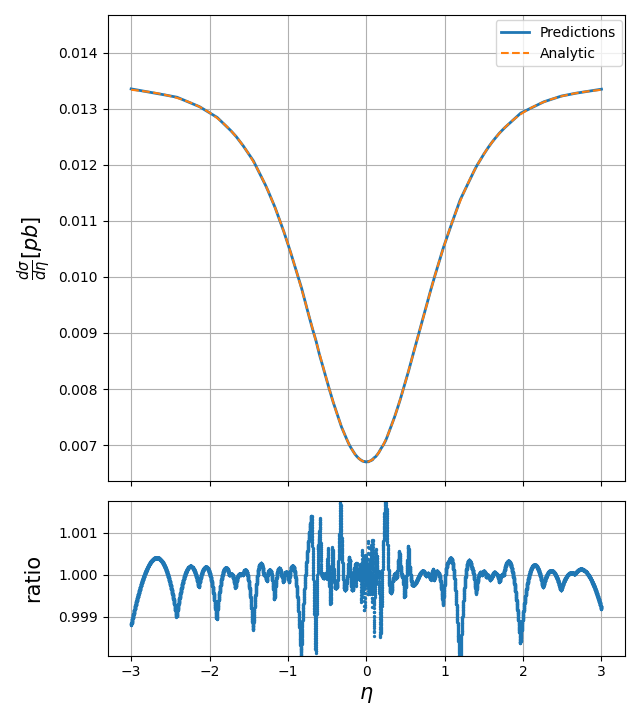
\includegraphics[width=8cm]{graphics/partonic_eta_model_eta_ratio}
	\caption{machine learning predictions vs analtisch berechnete Werte Eta}
	\label{partonic_eta_model}
\end{figure}
 \\
 \\
\textbf{Modell für $\mathbf{\frac{d\sigma}{d\theta}}$:} \\
Der Wirkungsquerschnitt in Abhängigkeit von $\theta$ unterscheidet sich vom vorherigen Modell durch seine Polstellen. Da Computer schlecht mit Polstellen umgehen können, müssen wir den Trainingsbereich auf $[\epsilon, \pi-\epsilon]$ einschränken. Aus physikalischer Sicht ist das legitim, da die Polstellen im Strahlengang des Speicherrings liegen und damit nicht messbar sind. Viele Detektoren können Pseudo-Rapiditäten bis zu $\abs{\eta} \leq 2.5$ messen, was einem $\epsilon \approx 0.163$ entspricht. Man kann dem Modell den Umgang mit den Polstellen erleichtern, in dem man die Labels(also den differentiellen Wirkungsquerschnitt) auf das Intervall $[-1, 1]$ normiert. Da gute Modelle hier nicht mehr trivial gefunden werden können, greifen wir auf eine automatische, zufällige Suche zurück (Random-Search), um nicht einzelne Hyperparameter per Hand ausprobieren zu müssen. Die Such-Parameter mit Ergebnis sind in \textit{\autoref{text}} festgehalten.

Es fällt auf, dass die Architektur des Modells um ein vielfaches komplizierter ist, als die vorhergehende. Einerseits ist dies aufgrund der Polstellen zu erwarten und andererseits ist die Möglichkeit des Overfitten durch die große Anzahl an Trainingspunkten weitgehend ausgeschlossen und daher nur natürlich, dass komplexere Modelle genauere Ergebnisse erzielen. Die Performance des Modells ist in \textit{}\autoref{label} gezeigt. Die Präzision ist trotz der komplizierteren Funktion mit \textit{\autoref{text}} zu vergleichen. Durch den Random-Search konnte also ein vergleichsweise passendes Modell gefunden werden. \\
\begin{figure}[tbp]
	\centering
	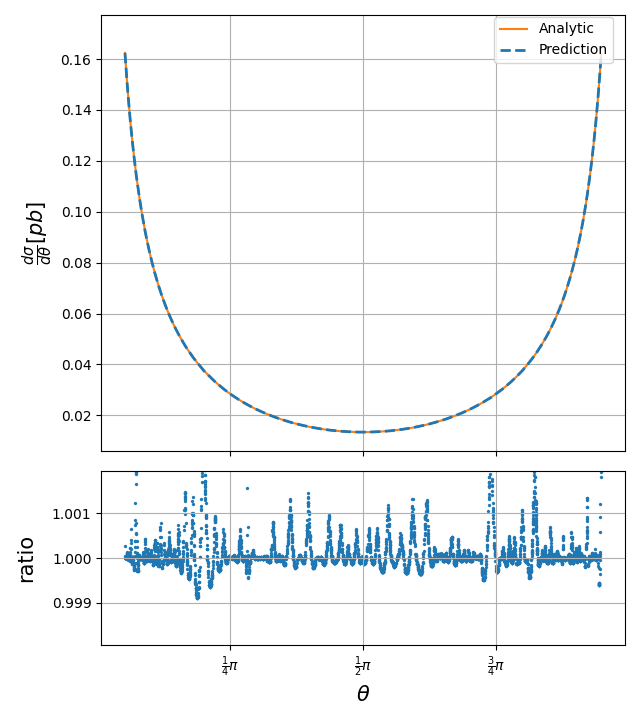
\includegraphics[width=8cm]{graphics/2}
	\caption{Predictions vs Analytisch auf relevantem Theta-Intervall}
\end{figure}
Wir wollen nun betrachten, wie sich das Modell auf einem Interval $[\epsilon', \pi-\epsilon']$ mit $\epsilon' < \epsilon$ schlägt. Wir vergleichen dies mit einem Modell, dass zwar mit den gleichen Hyperparametern, jedoch auf $[\epsilon', \pi-\epsilon']$ trainiert wurde. Für ein drittes Modell sind die Trainingsdaten nach einer Verteilung generiert, die der Form von $\frac{d\sigma}{d\theta}$ ähnelt (Importance Sampling). Die Vergleiche sind in \textit{\autoref{text}} und in \textit{\autoref{text}} für $\epsilon' = 0.01$ gezeigt. Wie zu erwarten weicht das ursprüngliche schnell von der analytischen Funktion ab. Man erkennt, dass dem Modell zwar die Tendenz bekannt ist, der genaue Verlauf jedoch rasch unbekannt wird. Man könnte vermuten, dass der Maschine zwar die Steigung bekannt ist, alle weiteren Ableitungen jedoch die Komplexität des Modells übertreffen. Die beiden anderen Modelle zeigen akzeptable Leistung auch nahe an den Polstellen. In \textit{\autoref{text}} lässt sich schlecht beurteilen, ob das importance Sampling Wirkung zeigt. Lediglich im Verhältnis kann man erahnen, dass das mit importance gesampelten Trainingsdaten trainierte Netz an den Polstellen besser und im Zentrum schlechter angepasst ist. In \textit{\autoref{text}} a) wird diese Vermutung bestätigt, auch wenn die Auswirkungen nur vergleichsweise klein sind. Einen größeren Effekt sieht man in \textit{\autoref{text}} b). Durch die große Zahl an Trainingsdaten in a) sind schon genug Punkte nahe an der Polstelle vorhanden und die zusätzlichen Werte bringen nur einen kleinen (absoluten) Mehrwert. Ist man jedoch begrenzt in seiner Verfügung über Trainingsdaten oder möchte die Trainigszeit minimieren und trotzdem brauchbare Ergebnisse erhalten, kann importance sampling jedoch helfen. Man sollte jedoch im Hinterkopf behalten, dass man hierbei einen Kompromiss eingeht und die Verlässlichkeit in den Bereichen, die durch das sampling vernachlässigt werden, abnimmt. 
In \textit{\autoref{text}} sind noch einmal der MAPE (Mean-Absolute-Percentage-Error) der verschiedenen Modell für verschiende Testdatensets gezeigt. Hier wird noch einmal deutlich, dass das importance sampling vor allem nützlich ist, wenn die Bereiche von Funktionen besonders wichtig sind, in denen die Funktion auch einen hohen Funktionswert besitzt. Da wir den differentiellen Wirkungsquerschnitt letztendlich benutzen wollen, um den totalen Wirkungsquerschnitt zu berechnen, ist dies für uns genau der Fall. Allgemein geht das Annähern eines beliebigen Integranden mittels maschinellem Lernen Hand in Hand mit anschließender Monte-Carlo Integration. Die Verteilung, die wir benutzen, um die Form des Wirkungsquerschnittes anzunähern, ist die ein Polynom vierten Grades und in \textit{\autoref{text}} gezeigt.
\begin{figure}[tbp]
	\centering
	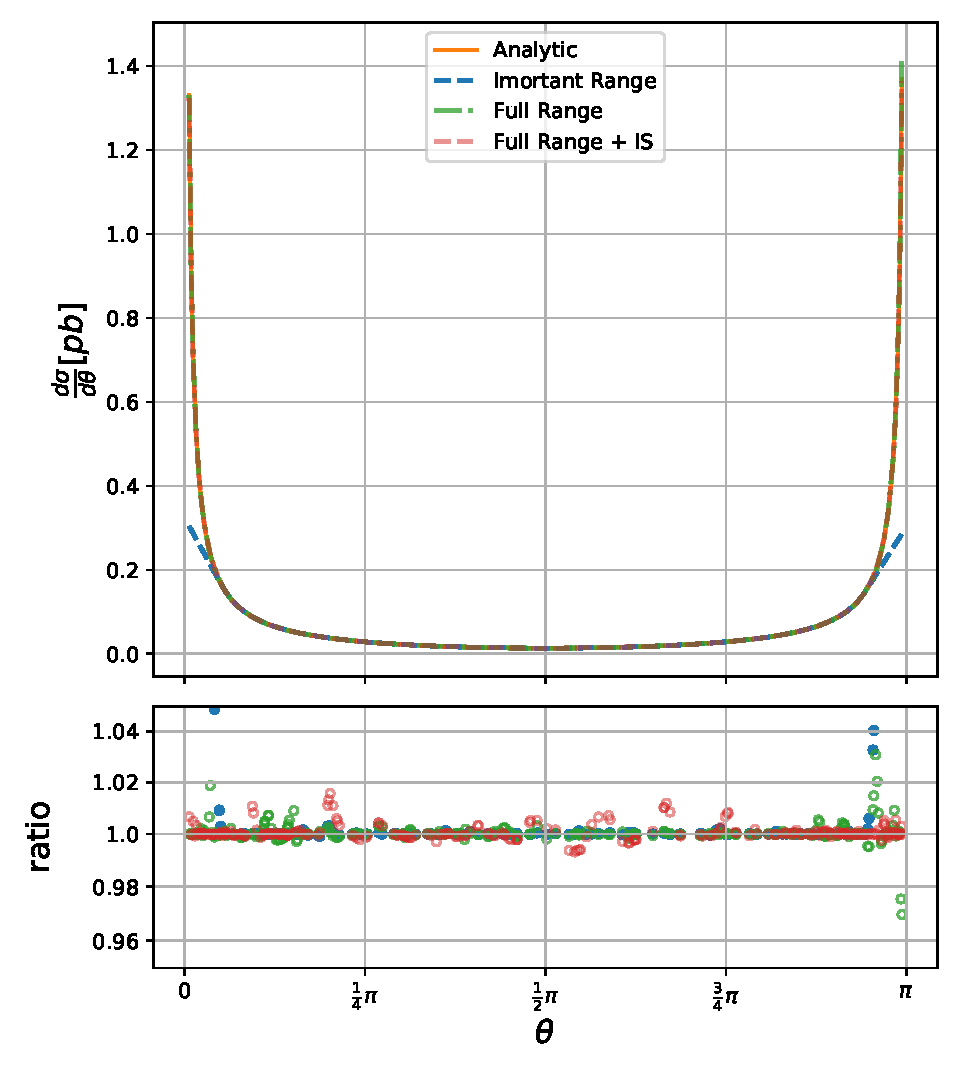
\includegraphics[width=9cm]{graphics/3}
	\caption{machine learning predictions vs analtisch berechnete Werte}
	\label{partonic_theta_model}
\end{figure}
\begin{figure}[tbp]
	\centering
	\subfloat[Modelle mit 60000 Traningspunkten]{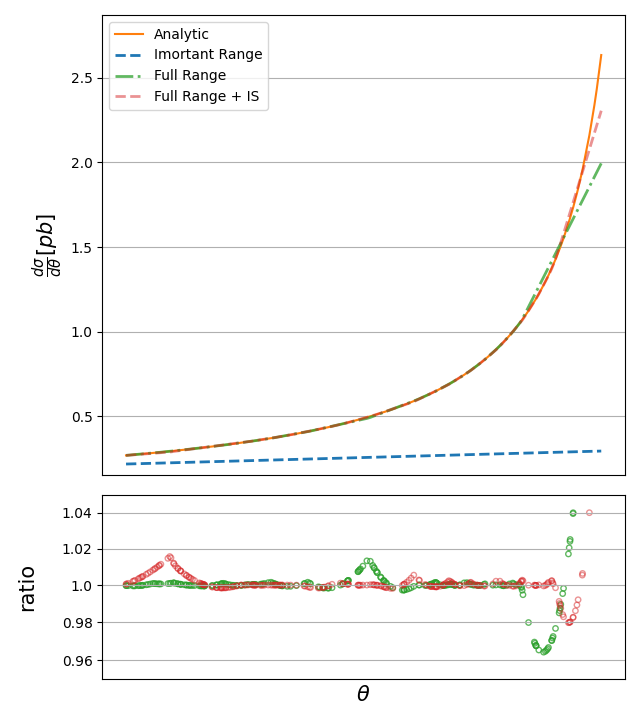
\includegraphics[width=7cm]{graphics/3.1}}
	\subfloat[Modelle mit 10000 Trainingspunkten]{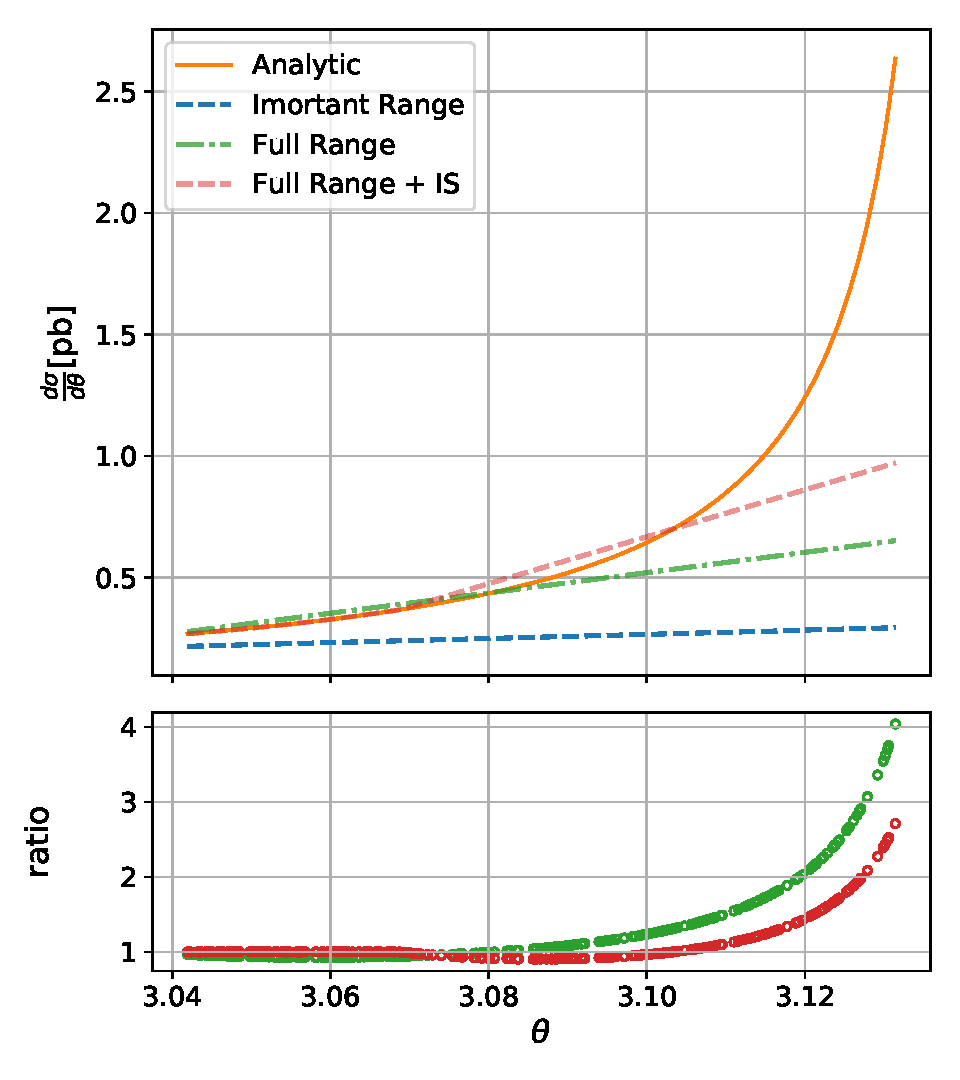
\includegraphics[width=7cm]{graphics/3.2}}
	\caption{Performance des Netzes für Randpunkte}
	\label{3.1 / 3.2}
\end{figure}
\begin{figure}
	\centering
	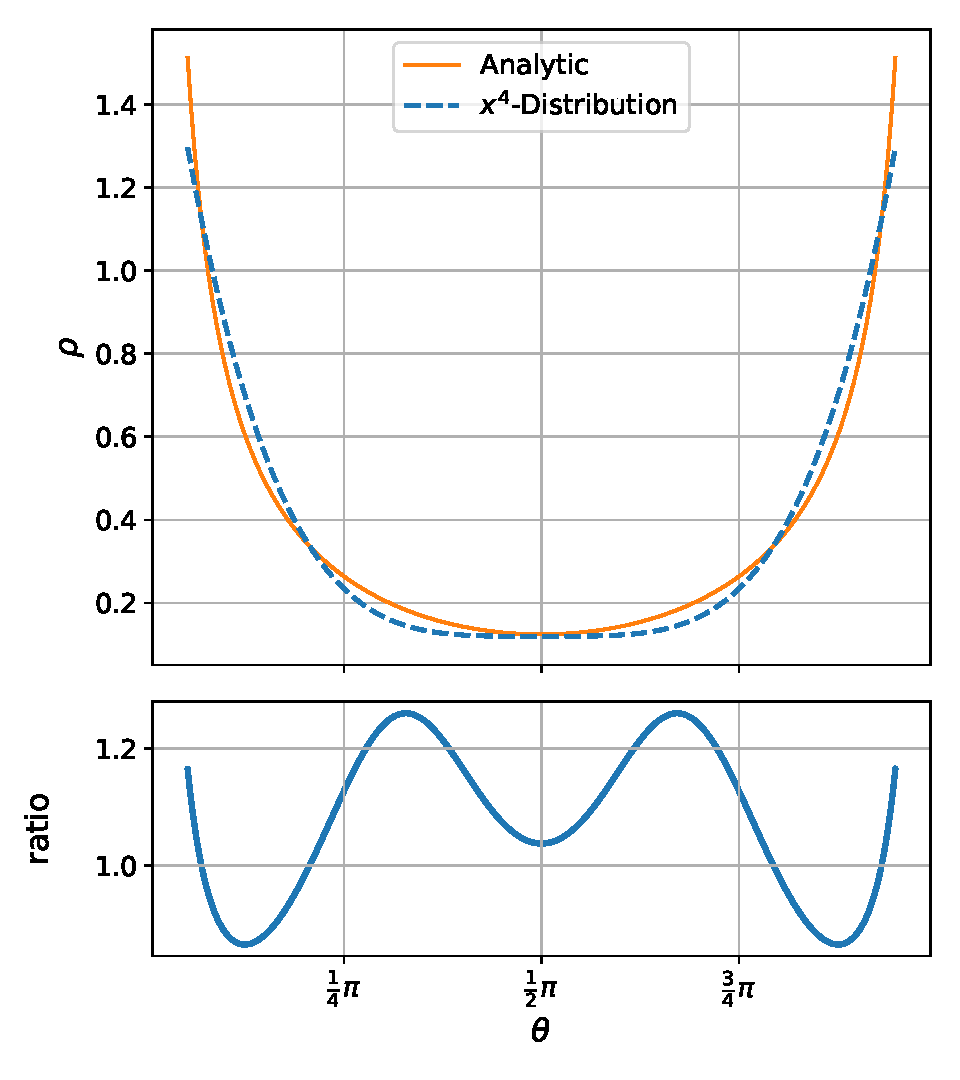
\includegraphics[width=8cm]{graphics/4}
	\caption{simples Importance Sampling, das die analytische Funktion annähern soll}
\end{figure}
\begin{figure}
	\centering
	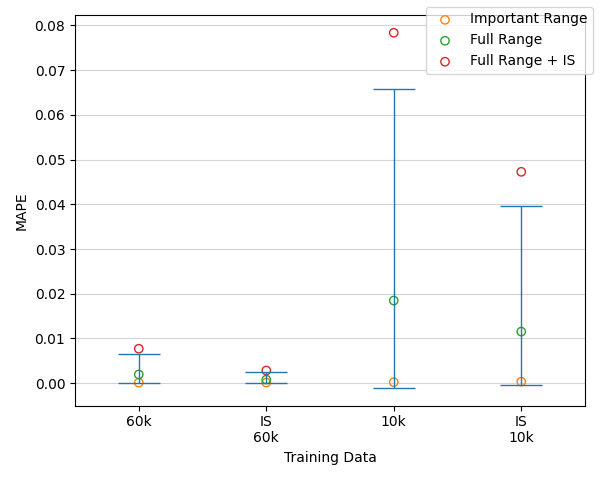
\includegraphics[width=9cm]{graphics/26}
	\caption{Vergleich der Performance von verschiedenen Theta-Modellen, die mit verschiedenen Datenmengen trainiert wurden. IS: Importance sampling. Auf der x-Achse sind die Trainings-Datenmengen und in der Legende die Test-Datenmengen}
\end{figure}
\section{Hadronischer Diphoton-Prozess}
\subsection{cuts and stuff}
Im Gegensatz zu den im Vorhergehenden betrachteten Prozessen, ist die Reaktion $pp \rightarrow \gamma \gamma$ beobachtbar und messbar. Wir wollen den Wirkungsquerschnitt am Beispiel einer Messung im ATLAS-Detektor behandeln. Da kein Detektor perfekt ist, müssen wir die Events nach messbaren und nicht-detektierbaren Ereignissen einteilen. Wir wenden also Cuts auf unsere generierten Phasenraumpunkte an und trainieren unseren Algorithmus nur an solchen Messpunkten, die auch praktisch detektierbar wären. Die verwendeten Cuts sind angelehnt an \textit{\autoref{Siegert}} und aufgelistet in \textit{\autoref{label}}.
\begin{table}
	\centering
	\begin{tabular}{|c|c|}
		\hline
		Bereich & Cut \\
		\hline
		Photon-Energie & $\abs{p_T} > 40$ GeV \\
		Photon Winkel & $\abs{\eta_{\gamma, \tilde{\gamma}}} < 2.37$ ohne $¸1.37 < \abs{\eta_{\gamma, \tilde{\gamma}}} < 1.52$ \\
		Impulsbruchteil & $x_{1,2} < 0.7 $\\
		\hline
	\end{tabular}
	\caption{Event-Selektion für den Diphoton-Prozess in Leading-Order am ATLAS - Detektor}
\end{table}
Dabei sind $\gamma$ und $\tilde{\gamma}$ die Bezeichnungen für die beiden Photonen. $p_T$ bezeichnet dabei den Impuls der produzierten Photonen transversal zum Strahlengang. Da die Quarks, die im Prozess beteiligt sind in unserem Modell nur einen Impuls in Strahlrichtung haben, folgt aus der Impulserhaltung direkt $p_{T,\gamma} = p_{T,\tilde{\gamma}}$. ATLAS kann keine beliebig spitzen Winkel messen, daher betrachten wir nur Photonen mit einer Pseudo-Rapidität von $\eta < 2.37$. Der Detektor besteht aus zwei Teilen, wobei sich der eine Teil wie ein Zylindermantel um den Strahl legt und der andere die Deckel darstellt. Zwischen diesen Teilen befindet sich ein Spalt, in dem nicht gemessen werden kann, daher verwerfen wir auch Ereignisse mit $1.37 < \abs{\eta_{\gamma, \tilde{\gamma}}} < 1.52$. Wie wir später sehen werden, machen die Partondichtefunktionen und damit auch der dreifach differentielle Wirkungsquerschnitt ab ca. $x \approx 0.7$ einen Bogen und fällt extrem schnell zu Null hin ab. Zum totalen Wirkunsquerschnitt, der letztendlich unser Ziel darstellt, trägt dieser Bereich so gut wie nicht mehr bei. Weiterhin vereinfacht es es dem neuronalen Netz extrem, wenn er diesen Phasenraumbereich mit extrem kleinen Labels nicht mehr erlernen muss.
\newline
%TODO graph der deine eta Rechnung erklärt?
Wir müssen weiterhin beachten, dass wir beide Photonen messen können müssen, damit wir den Prozess identifizieren können. Da wir im Schwerpunktsystem der Protonen messen, unterscheiden sich die Pseudo-Rapiditäten der beiden Photonen. Wir müssen die Cuts in $\eta$ also für beide Photonen sicherstellen. Messen wir sowohl $\eta_{\gamma}$ als auch $\eta_{\tilde{\gamma}}$ in Bewegungsrichtung des Quarks mit Impulsbruchteil $x_1$, berechnet sich $\eta_{\gamma}$ aus dem $\eta'$ der Photonen im Schwerpunktsystem der Quarks nach \textit{\autoref{text}}.
\begin{equation}
	\eta_{\gamma} = \eta' -\frac{1}{2}\ln(\frac{x_2}{x_1}) \quad \text{sowie} \quad \eta_{\tilde{\gamma}} = -\eta’ - \frac{1}{2}\ln(\frac{x_2}{x_1})
\end{equation}
Intuitiver ist es jedoch, wenn $\eta_{\gamma} = \eta_{\tilde{\gamma}} für x_1 = x_2$ gelten würde, anstatt $\eta_{\gamma} = - \eta_{\tilde{\gamma}}$, sprich wenn wir $\eta_{\tilde{\gamma}}$ in Bewegungsrichtung von $x_2$ messen würden. Dabei transformiert sich $\eta_{\tilde{\gamma}} \rightarrow -\eta_{\tilde{\gamma}}$ und wir finden \textit{\autoref{text}}.
\begin{equation}
	\eta_{\tilde{\gamma}} = \eta’ + \frac{1}{2}\ln(\frac{x_2}{x_1}) \quad \Rightarrow \quad \eta_{\tilde{\gamma}} = \eta_{\gamma} + \frac{1}{2}  \ln(\frac{x_2^2}{x_1^2})
\end{equation}
\subsection{Suchprozess}
Den Integranden den wir nun erlernen möchten (\textit{\autoref{text}}) ist nun nicht mehr eindimensional, sondern dreidimensional. Dieser Unterschied fällt zwar zunächst als erstes auf, es ist jedoch ein anderer Faktor, der das neuronale Netz stärker beeinflusst. Die Partondichtefunktionen, die den dreidimensionalen Wirkungsquerschnitt bestimmen, fallen exponentiell mit ihren Impulsbruchteilen $x_1$ und $x_2$ ab und besitzen Polstellen für $x \rightarrow 0$. Damit man numerisch mit den Partondichtefunktionen auch noch an der Stelle Null arbeiten kann, werden diese ab einem gewissen $x_{min} \approx 10^{-9}]$ eingefroren. Praktisch heißt das jetzt, dass sich unsere Labels zwischen ca 30 Größenordnungen bewegen. Mit derartigen Veränderungen können neuronale Netze nicht arbeiten, da diese Formen allein schon konzeptionell nicht zu erreichen sind. Das wird intuitiv, wenn man sich das neuronale Netz als eine Reihe an hintereinander ausgeführten Matrixmultiplikationen vorstellt, die nur ihre Linearität dank den Aktivierungsfunktionen verlieren. Die Sensitivität auf kleine Veränderungen in $x$ ist so nur begrenzt zu reproduzieren. Hinzu kommt, dass eine gängige Loss-Funktion wie der Mean-Squared- oder Mean-Absolute-Error offensichtlich nur Punkte mit hohen Wirkungsquerschnitten berücksichtigen und damit die Ergebnisse schon ab einem kleinen $x$ unbrauchbar werden würden. Abhilfe kann hierbei die oft für ähnliche Probleme verwendete Loss-Funktion \glqq Mean-Squared-Logarithmic-Error(MSLE)\grqq~ schaffen (siehe \textit{\autoref{text}}). Wir sehen, dass es beim MSLE nicht mehr auf die Größe der Abweichung ankommt, sondern das Verhältnis der Werte. Damit ist gesichert, dass keine Bereiche des Phasenraumes komplett vernachlässigt werden. Um nicht mit negativen Werten zu arbeiten, transformiert man meistens $y \rightarrow y + 1$. Diese Form hilft uns jedoch nicht weiter, da der Großteil unserer numerischen Werten in herkömmlich verwendeten Einheiten sprich $1/\text{GeV}^2$ und $\text{pb}$ viel kleiner als eins ist. Bemühen wir die Taylor-Entwicklung des Logarithmus um eins, fällt auf, dass $\ln(1+x) \approx x$ gilt und wir somit effektiv nur einen ineffizienteren Mean-Squared-Error implementieren. 
\begin{equation}
	C\left(\mathbf{M}, \mathbf{b}\right) = \frac{1}{N} \sum_{i=1}^{N} \left(\ln(y^{(i)}) - \ln(\tilde{y}^{(i)})\right)^2 = \frac{1}{N} \sum_{i=1}^{N} \left(\ln(\frac{y^{(i)})}{\tilde{y}^{(i)}})\right)^2
\end{equation}
Hier kommt die Skalierung, die wir in den beiden vorhergehenden Modellen bereits verwendet haben, ins Spiel. Die Skalierung beseitigt außerdem das \glqq Dying-ReLU\grqq- Problem, dass im Zusammenhang mit numerisch kleinen Labels auftreten kann. Es geht hierbei um einen großen Gradienten nach Überschätzung der Funktionswerte seitens des Netzes, der auf die Neuronen angewendet wird und die Parameter so verändert, dass das Neuron in der Zukunft nur noch Null zurückgeben wird. Da im Bereich der ReLU unter Null auch die Ableitung der Loss-Funktion Null ist, kann sich die Node somit nicht regenerieren. Das passiert bei sehr kleinen Labels schon nach den ersten Batches, da die durch Initialisierung der Gewichte der Layer, das Modell zu Beginn des Trainings einen mehr oder weniger zufälligen Wert zurückgibt. Man müsste also die Initialisierung der Gewichte perfekt auf die vorliegenden Daten abstimmen, falls das überhaupt im vorliegenden Fall möglich ist. Es ist also naheliegend auf die Skalierung der Funktionswerte zurückzugreifen. Praktisch wird das bei uns durch einen Transformator-Objekt realisiert, der die vorliegenden Labels so skaliert, dass der kleinste Funktionswert auf eins abgebildet wird. Die Skalierungskonstante hängt offensichtlich von den vorliegenden Phasenraumpunkten ab und ist damit von Datenset zu Datenset unterschiedlich. Daher erstellen wir im folgenden für jeden für jedes Modell einen zugehörigen Transformator, der nach dem Training mit dem Modell abgespeichert wird und bei Bedarf wieder initialisiert werden kann. Die Skalierungskonstante ist wichtig, damit wir später unabhängig vom Trainingsdatenset die Predictions unseres Modells auf die wirklichen Werte zurückskalieren können. Weitere Möglichkeiten um mit dem \glqq Dying-ReLU\grqq-Problem umzugehen sind die Verwendung von Aktivierungsfunktionen mit nicht-verschwindender Ableitung wie Leaky-ReLU oder ELU, die den Nodes ermöglichen soll, sich zu regenerieren, oder die Übergabe eines \glqq  Clipvalue/Clipnorm\grqq-Parameters an den Optimizer, der den Gradienten reguliert. 
Die Skalierung in Kombination mit dem Mean-Squared-Logarihmic-Error macht eine Anwendung von tiefen neuronalen Netzen auf das vorliegende Problem überhaupt erst möglich. Wir werden später die Transformation der vorliegenden Daten und deren Effekt auf das Lernverhalten der Netze genauer untersuchen. Da wir nun bereits einen Transformator verwenden, müssen wir das bilden des Logarithmus auch nicht mehr auf die Loss-Function abwälzen. Wir können nun das Netz direkt den Logarithmus der Wirkungsquerschnitte lernen lassen und haben alle nötigen Informationen zur Rücktransformation der Ausgaben des Netzes im Transformator gespeichert. So können wir den Komfort der in Keras implementierten Loss-Funktionen verwenden und müssen keine eigenen Implementationen kreieren, sobald wir beispielsweise einen Mean-Absolute-Logarithmic-Error verwenden wollen. Die Label-Normalisierung aus dem vohergehenden Modell wurde praktisch auch im Transformator umgesetzt.
\newline
Selbst mit den eingeführten Transformierungen ist das Erlernen jedoch immer noch keine triviale Aufgabe. Zur Hyperparameteroptimierung verwenden wir wieder einen Random Search. Für die Hyperparameter wurden mittlereweile zwar Algorithmen entwickelt, die effizienter sein sollen als ein Random Search, in dieser Arbeit konnte jedoch keine Verbesserung festgestellt werden. Konkret ausprobiert wurden ein "Bayesian Search" und der "Hyperband-Tuner", wobei die Implementierung mit Keras-Tuner vollzogen wurde. Bayesian Search benutzt eine Objecitv-Funktion, die aus den bereits getesteten Hyperparametern eine Vorhersage für vielversprechende neue Hyperparameter-Kombinationen abgibt. Hyperband trainiert eine große Zahl an Modellen für wenige Epochen und sucht aus diesen die besten Kandidaten zum Weitertrainieren aus. Dies wird stufenweise durchgeführt, bis man in der Theorie mit einer Hand voll gut funktionierender Hyperparameter zurückbleibt. Die Hyperparameter einer erfolgreichen Suche sind in \textit{\autoref{text}} aufgelistet.

Hierbei muss man beachten, dass die Trainingspunkte zufällig generiert sind nach den Verteilungen in \textit{\autoref{text}}. 
\begin{equation}
	\begin{aligned}
	\rho(x) &= \frac{1}{(x + \alpha)\ln(\frac{x_{max} + \alpha}{x_{min}+ \alpha})} \qquad \text{mit} \qquad \alpha = 0.005 \\
	\rho(\eta) &= \begin{cases}
	\frac{1}{\sqrt{2\pi \sigma^2}} \exp(-\frac{(\eta - \eta_{max})^2}{2\sigma^2}) \quad & \text{für} \qquad 0 \leq \eta \leq \eta_{max}\\
	\frac{1}{\sqrt{2\pi \sigma^2}} \exp(-\frac{(\eta + \eta_{max})^2}{2\sigma^2}) \quad & \text{für} \quad -\eta_{max} \leq \eta < 0
	\end{cases} \quad \text{mit} \quad \sigma = 1.5
	\end{aligned}
\end{equation}
Nach der Generation müssen wir jedoch die Cuts aus \textit{\autoref{text}} anwenden. Bei gegebenen Parametern und Cuts beläuft sich dabei die Sample-Effizienz auf $\approx 40\%$. Wir trainieren also mit weniger Daten, als es auf den ersten Blick wirkt. Das Sampling entspricht einem Importance-Sampling, dessen Nutzen schon im vorigen Abschnitt besprochen wurde. 
%TODO Umrechnung in pb für Grafik 8
\begin{figure}[tbp]
	\centering
	\subfloat[]{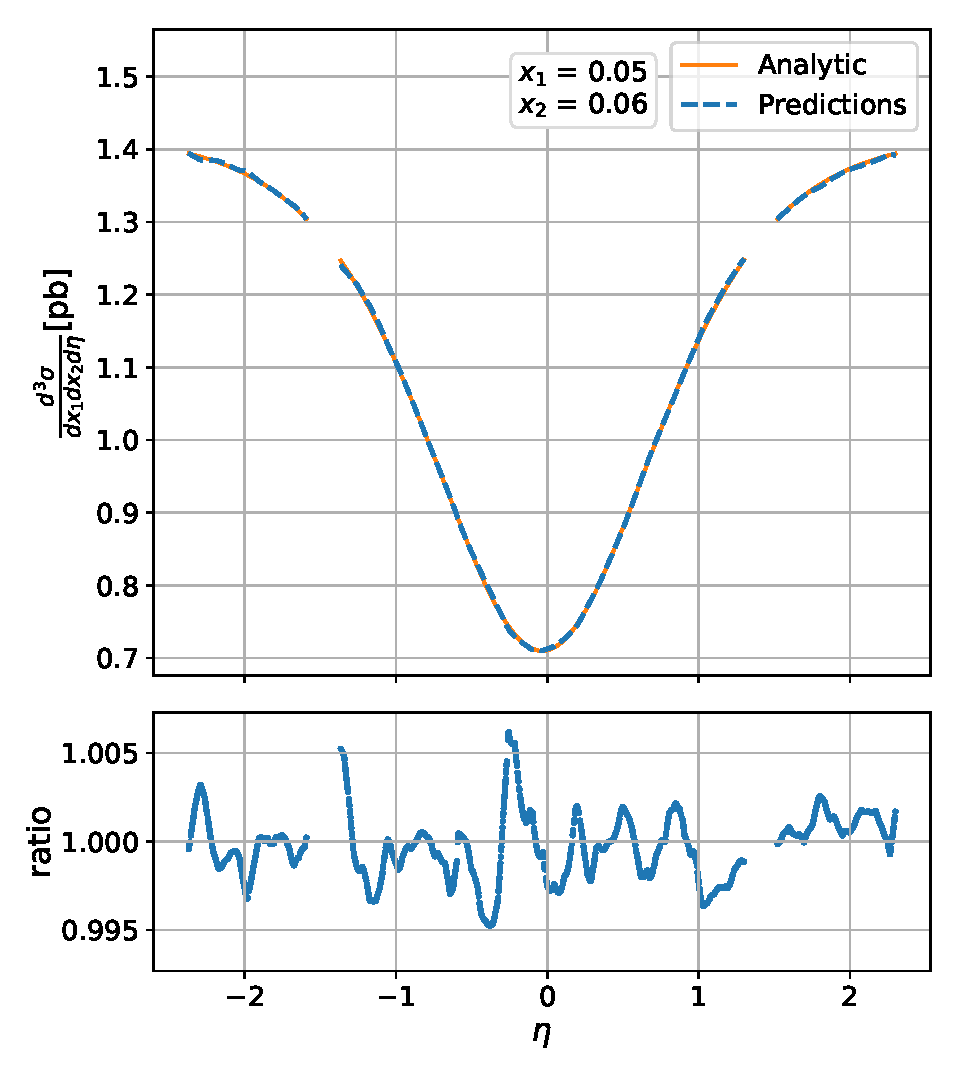
\includegraphics[width=7cm]{graphics/5}}
	\subfloat[]{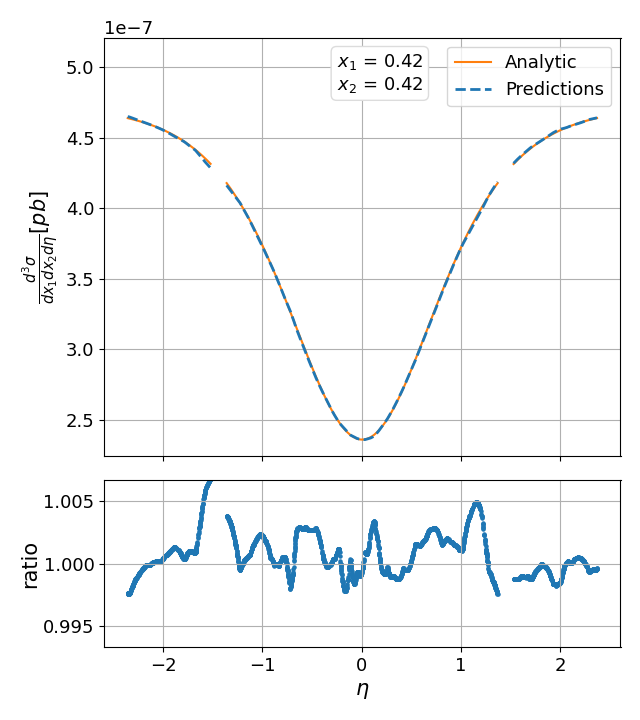
\includegraphics[width=7cm]{graphics/8}}
	\caption{Schnitte des differentiellen Wirkungsquerschnitts in $\eta$}
	\label{5,8}
\end{figure}
\begin{figure}[tbp]
	\centering
	\subfloat[]{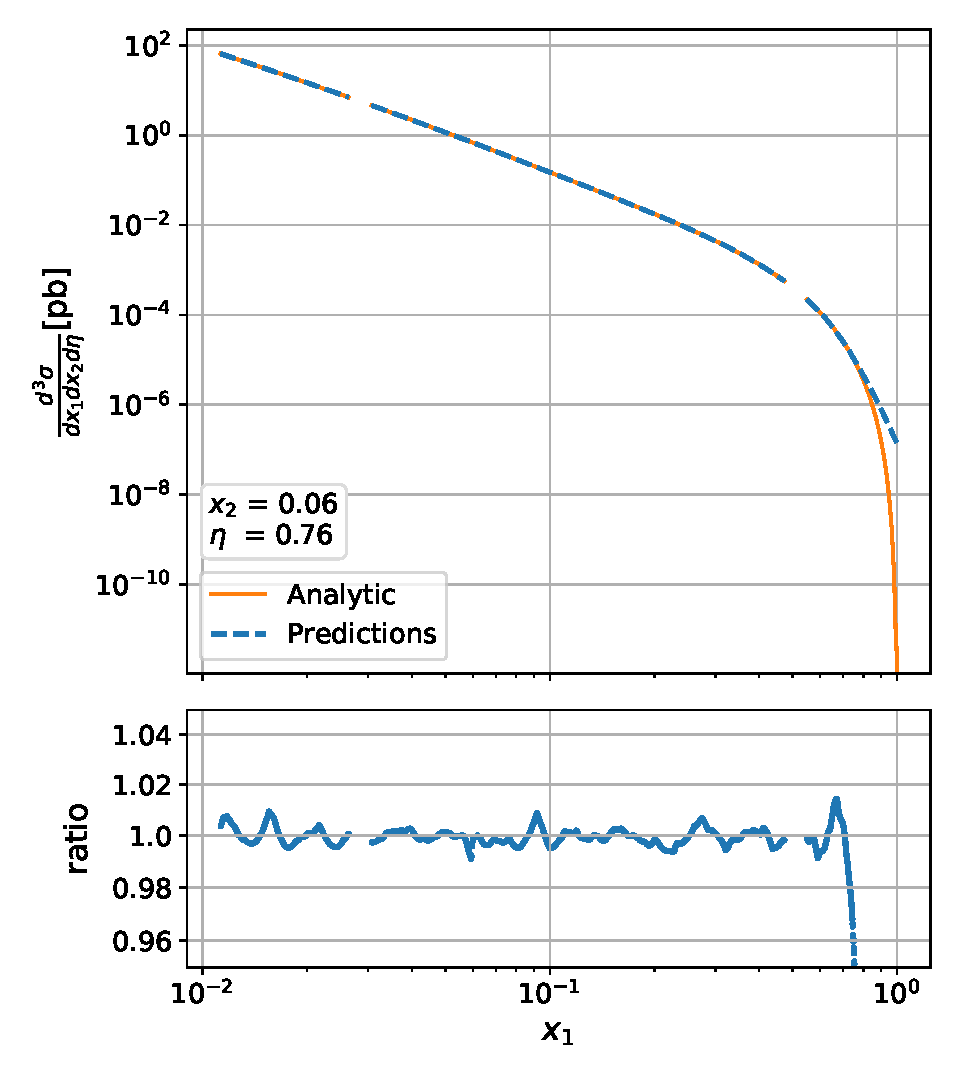
\includegraphics[width=7cm]{graphics/6}}
	\subfloat[]{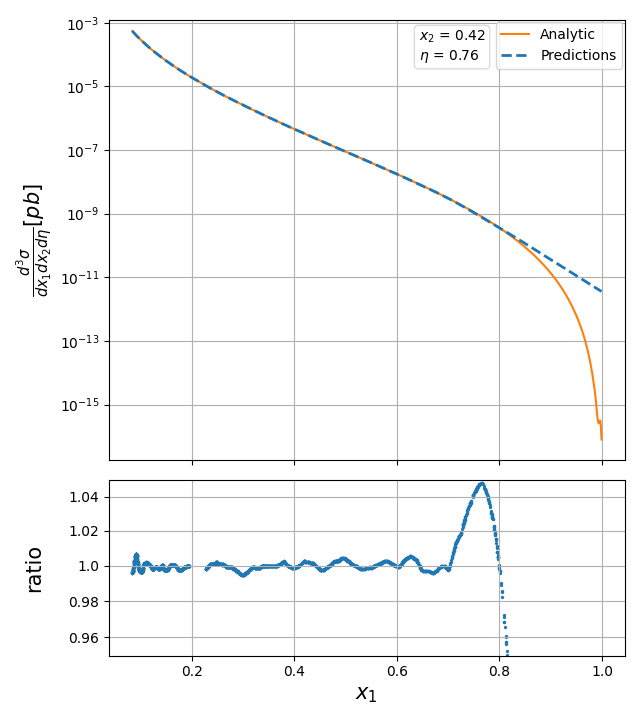
\includegraphics[width=7cm]{graphics/9}}
	\caption{Schnitte des differentiellen Wirkungsquerschnitts in $x_1$}
	\label{6,9}
\end{figure}
\begin{figure}[tbp]
	\centering
	\subfloat[]{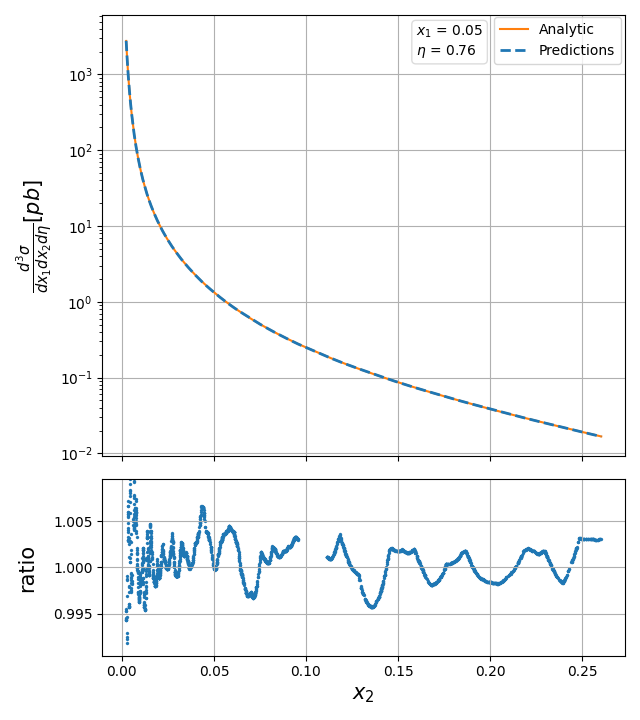
\includegraphics[width=7cm]{graphics/7}}
	\subfloat[]{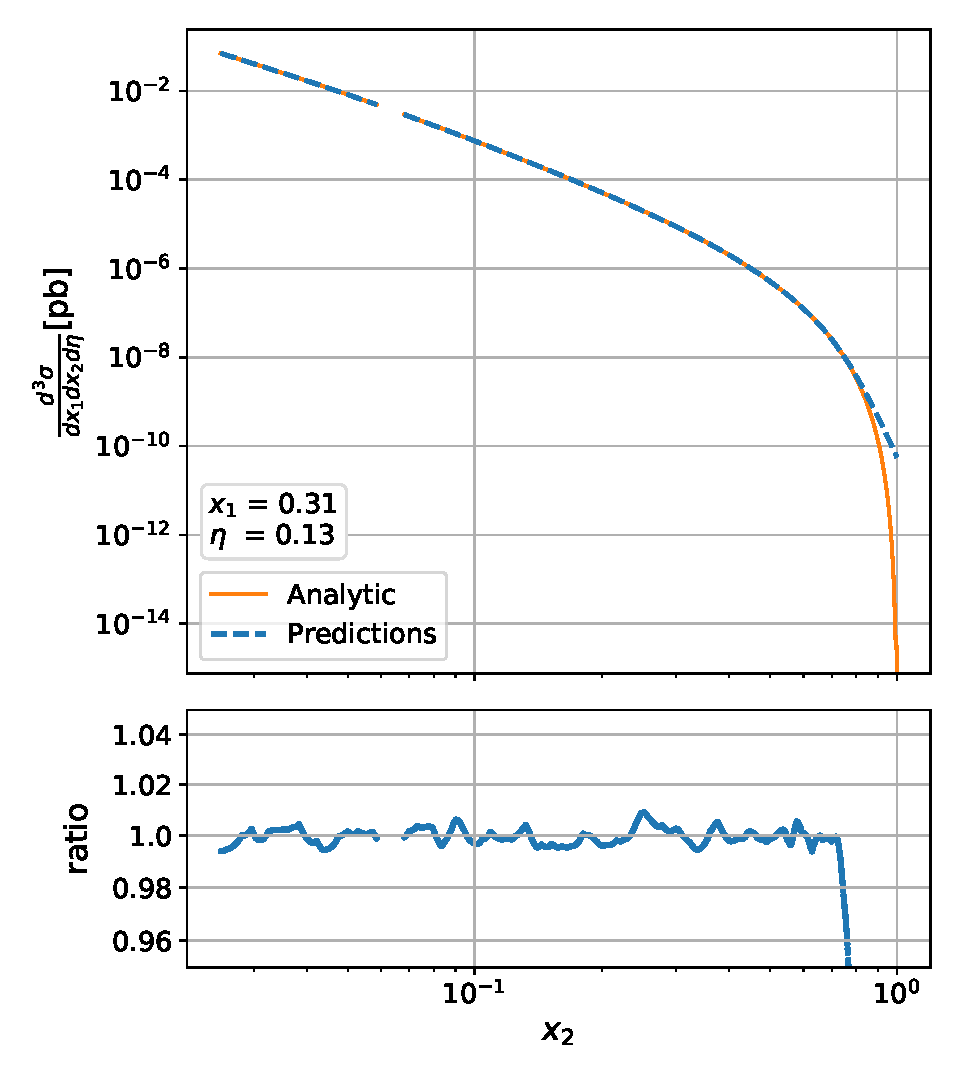
\includegraphics[width=7cm]{graphics/10}}
	\caption{Schnitte des differentiellen Wirkungsquerschnitts in $x_2$}
	\label{7,10}
\end{figure}
In den Abbildungen \textit{\autoref{text}}, \textit{\autoref{text}},... sind Schnitte des dreidimensionalen Wirkungsquerschnittes an verschiedenen Phasenpunkten gezeigt. Wir sehen, dass sich unsere intensive Behandlung der Hyperparameter und der Daten-Transformationen bezahlt gemacht hat. Wir verzeichnen an den meisten Stellen eine maximale Abweichung von lediglich $0.5\%$. Für Ausnahmefälle beträgt die Abweichung bis zu $\approx 1\%$. Es lässt sich leicht der Moment erkennen, ab dem die x-Werte gefiltert wurden. Wie schon im Modell für $\frac{d\sigma}{d\theta}$, verläuft die Vorhersage des Modells linear weiter und entfernt sich somit von den analytischen Werten. Für große $x$ wird unser Modell also den Wirkungsquerschnitt gegebenenfalls um Größenordnungen überschätzen. Da jedoch nur der integrierte Wirkungsquerschnitt über $x_1, x_2$ überhaupt messbar ist und dieser sich nicht merklich durch diese Abweichung beeinflussen lässt, ist es gerechtfertigt in diesem Phasenraumbereich eine so große Abweichung zu besitzen. 
\subsection{Vergleiche}
Wir wollen nun noch einmal direkt die Performance der einzelnen Hyperparameter an unserem Problem untersuchen. Dafür benutzen wir die Konfiguration, die wir im Vorhergehenden durch den Random Search gefunden haben und variieren für jedes Training nur ein Hyperparameter. Für die Anzahl an Neuronen und Layern, die stark korreliert sind, ist die Veränderung eines einzelnen der beiden Parameter nur bedingt interessant. Daher vergleichen wir auch verschiedene Formen bzw. Architekturen des Netzes, sprich verschiedene Kombinationen von Anzahl an Layern und Units. Die Modell werden nach dem Mean-Absolute-Percentage Error eines Test-Datestets beurteilt, das genauso gesampelt ist wie die Trainingsdaten. Wir trainieren jedes Modell fünf mal mit unterschiedlichen Initialisierungen an zwei Millionen gesampelten Phasenraumpunkten, um die statistische Schwankung der Güte des Modells einschätzen zu können. Die eingezeichneten Fehlerbalken sollen die Schwankung verdeutlichen und sind kein Maß dafür, welchen Fehler das Netz in der Praxis erreichen kann. Ausreißer sind aus den Messungen herausfiltert, um die Lesbarkeit der Graphen zu gewährleisten. \\
\newline
\textbf{Loss-Funktion:}
In \textit{\autoref{text}} a) ist der Vergleich von drei verschiedenen Kostenfunktionen gezeigt. Für Probleme mit stark variierenden Labels setzt sich der Mean-Absolute-Error durch, da dieser nicht so sensitiv auf Ausreißer oder, in unserem Fall, Polstellen ist. Der Huber-Loss, der eine Kombination des linearen Fehlers und des quadratischen Fehlers darstellt, schlägt sich insgesamt besser als der reine quadratische Fehler, kann insgesamt jedoch nicht mit dem linearen Fehler mithalten. Das quadratische Verhalten des Fehlers für kleine Abweichungen scheint für unser Problem nicht von Vorteil zu sein.\\
\newline
\textbf{Optimizer:}
Der Vergleich des Optimizers \textit{\autoref{text}} b) überrascht, da generell der Adam-Optimizer in Literatur und auch erfahrungsgemäß die besten Ergebnisse liefert. Betrachtet man die Fehlerbalken, scheint es als, als würde für unser Problem RMSprop konstant etwas bessere Ergebnisse erzielen. Allerdings zeigt unsere Trainingsreihe für Adam einen Ausreißer. Um ein definites Ergebnis zu erhalten, welcher Optimizer für unser vorliegendes Problem besser geeignet is, müsste man größere Versuchsreihen aufnehmen. Nichtsdestotrotz sollte man RMSprop nicht von vornherein abschreiben, denn er ist ein Versuch Wert. Der normale Stochastic-Gradient-Descent erzielt signifikant schlechtere Ergebnisse. \\
\newline
\textbf{Trainingsdaten:}
Die Größe des Sets an Trainingsdaten ist in \textit{\autoref{text}} c) verglichen. Wie erwartet nimmt der Fehler des Modells mit der Zahl an vorhandenen Trainingsdaten ab. Das gleiche gilt voraussichtlich für die Unsicherheit auf dem Ergebnis, auch wenn in unserem Fall das Modell, das mit den meisten Trainingsdaten einen Ausreißer zeigt. Man erkennt jedoch auch, dass die Performance des Modells konvergiert und mehr als vier Millionen gesampelte Daten keinen signifikanten Beitrag mehr leisten. \\
\newline
\textbf{Learning-Rate:}
An dem Vergleich der Learning-Rates, der in \textit{\autoref{text}} gezeigt ist, kann man ein interessantes Verhalten des Netzes erkennen. Für eine Learning-Rate von $1 \cdot 10^{-3}$ verändert sich der mittlere Fehler so gut wie überhaupt nicht. Das deutet darauf hin, dass wir unabhängig von unserer Initialisierung bei dieser Learning-Rate das gleiche lokale Minimum finden. Die Abweichung der Performance wird danach mit der Learning-Rate größer, wir finden nun höhere und tiefere lokale Minima. Bei einer zu kleinen anfänglichen Lernrate, bleiben wir schon früh in einem hohen Minima stecken und können keine brauchbaren Ergebnisse erzielen. Wir können daraus schlussfolgern, dass es gut sein kann, seine anfängliche Learning-Rate etwas größer zu initialisieren, als man intuitiv für richtig halten würde. Dadurch kann man eine größere Menge an lokalen Minima erkunden, insofern man über die benötigte Rechenleistung verfügt. Beachte jedoch, dass dieser Ansatz nur in Kombination mit einem Zeitplan zur Reduzierung der Lernrate funktioniert und das \grqq Dying-ReLU\glqq~verstärken oder sogar auslösen kann. \\
\newline
\textbf{Daten-Transformationen:}
Welche Daten-Transformationen für unser Problem funktionieren, ist in \textit{\autoref{text}} gezeigt. Ich möchte an dieser Stelle noch einmal die Wichtigkeit dieser Transformationen hervorheben. Während man in der Literatur viel über die Normalisierung oder das Reskalieren der Features liest, werden die Labels oft von Transformationen ausgenommen. Für spezielle Regressionsprobleme, wie es bei uns vorliegt, können diese jedoch der Schlüssel dazu sein, überhaupt konvergierende Modelle zu erhalten. \textit{\autoref{text}} zeigt, dass verschiedene Implementationen brauchbare Ergebnisse liefern und es wichtiger ist, überhaupt die Skalierung und die Anwendung des Logarithmus zu verwenden. Trainingsläufe ohne Skalierung und Logarithmus sind nicht aufgeführt, da der Fehler nicht vergleichbar ist. Ein konvergierendes Modell ohne Logarithmus kann erhalten werden, wenn man anstelle des Logarithmus die Label-Normalisierung verwendet. \\
\newline
\textbf{Achitektur:} %TODO nr of layers ist nr der hidden layers ohne output oder normalisierung
Die Architektur in \textit{\autoref{text}} zu vergleichen ist interessant, da man sehen kann, dass eine passende Architektur zum Problem effektiver ist als die Komplexität des Modells. Das Modell mit den wenigsten zu trainierenden Parametern zeigt im Vergleich bessere Leistung als das komplexeste Modell. Die Modelle (128, 6), (256,5), (384, 4) zeigen unabhängig von ihren trainierbaren Parameter sehr gute Genauigkeit. Wir konnten also durch Orientierung am besten gefundenen Modell ein effizienteres finden, indem wir die Architektur ein wenig variiert haben. Das Modell (64, 7) zeigt trotz wenigen Freiheitsgraden akzeptable Genauigkeit. \\
% TODO trainable params unter die Architektur der Modelle
\newline
\textbf{Anzahl an Layer und Units pro Layer:} %TODO 64 als erstes bei units dann sieht es aus wie kurve
Sowohl für die Anzahl an Layer und der Units pro Layer verläuft nach einer Kurve, die ihr Minimum bei unseren optimalen Parametern hat. Der Schritt zum jeweils simpleren Modell ist klein und kann bei Bedarf einen Kompromiss zwischen Geschwindigkeit und Genauigkeit darstellen. \\
\newline
\textbf{Aktivierungsfunktionen:} %TODO Link zu den Abbildungen hier?
Die Abwandlungen der ReLU-Funktion zeigen sehr gute Ergebnisse, einsehbar in \textit{\autoref{text}}. Die gewöhnliche ReLU ist überraschenderweise etwas abgeschlagen. Eine plausible Erklärung hierfür liefert wiederum das \grqq Dying ReLU\grqq-Problem in Kombination mit unserer vergleichsweise hohen anfänglichen Lernrate.  \\
\newline
\textbf{Batch-Sizes:}
Auch die Batch-Sizes (siehe \textit{\autoref{text}}) haben große Auswirkungen auf das Lernverhalten des Modells. Ein Trainingsvorgang ist bei größerer Batch-Size mit passender Hardware zwar schneller, zeigt jedoch eindeutig größere Abweichungen. Aufgrund von zu wenigen Messdaten ist nicht klar, ob ein Modell, das mit großen Batches trainiert wird, in der gleichen Zeit, oder überhaupt, so tiefe Minima wie die kleineren erreichen können. 


\begin{figure}[tbp]
	\centering
	\subfloat[Vergleich für verschiedene Loss-Funktionen]{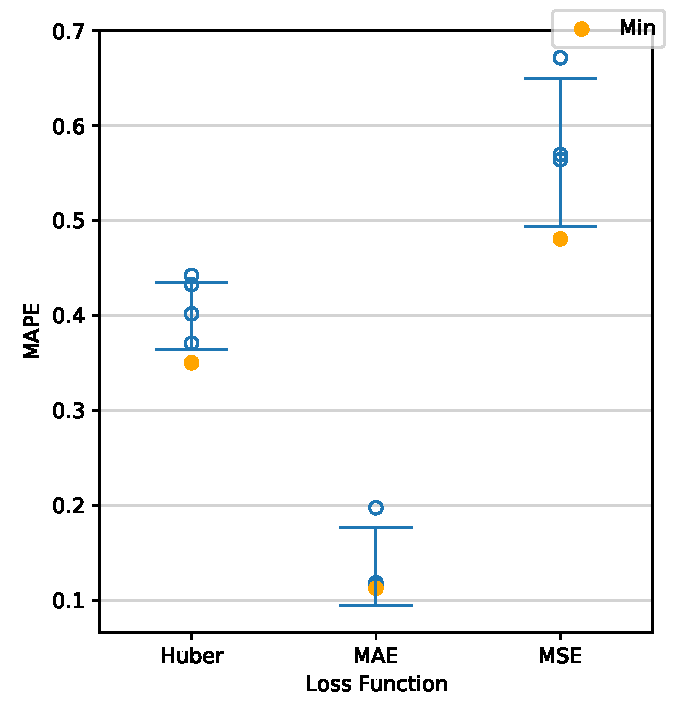
\includegraphics[width=7cm]{graphics/12}}
	\subfloat[Vergleich für verschiedene Optimizer \newline RMSprop,SGD mit $\text{momentum}= 0.1$]{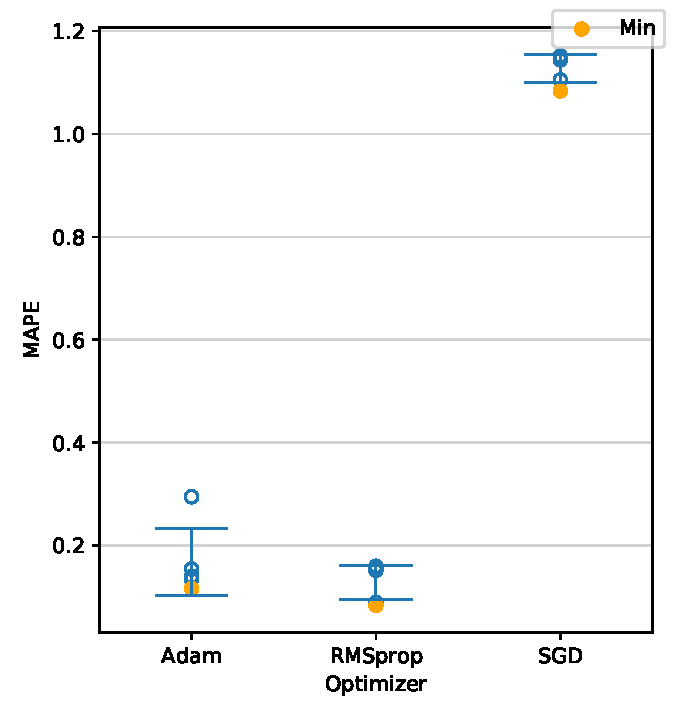
\includegraphics[width=7cm]{graphics/13}} \\
	\subfloat[Vergleich für verschiedene Anzahl an Trainigspunkten]{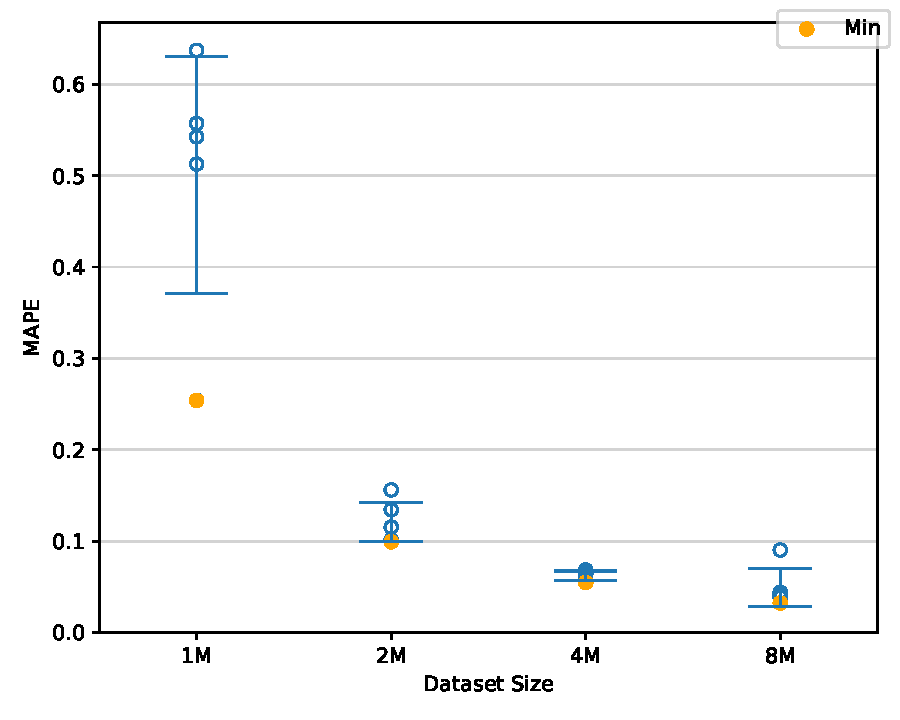
\includegraphics[width=7cm]{graphics/16}}
	\subfloat[Vergleich für verschiedene Anfangs-Lernraten]{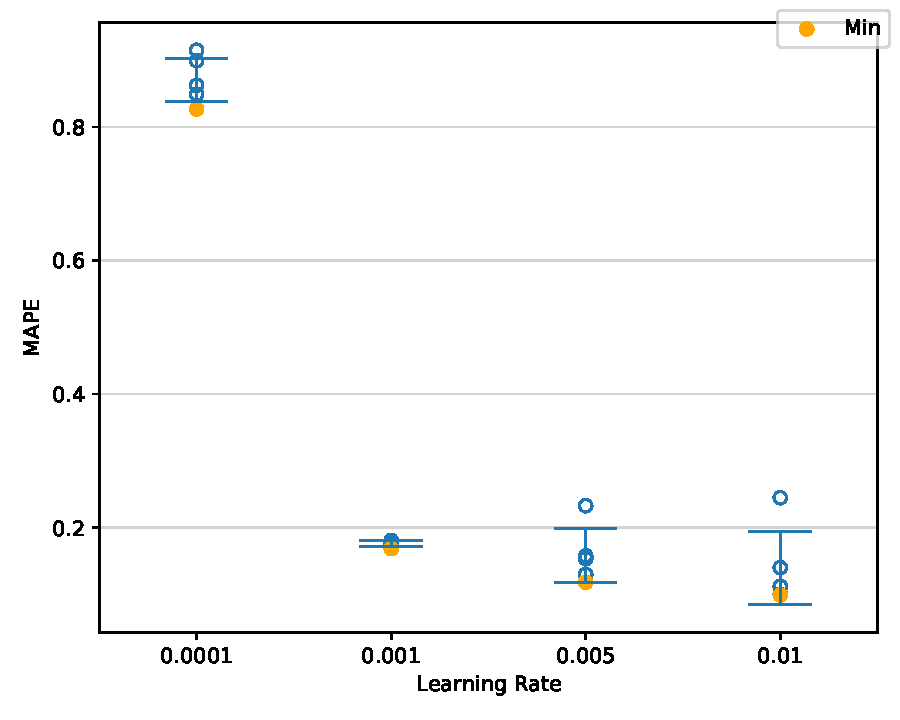
\includegraphics[width=7cm]{graphics/36}}
	\caption{Vergleich von Hyperparametern (I), MAPE: Mean-Absolute-Percentage-Error}
	\label{12,13,16,36}
\end{figure}
\begin{figure}[tbp]
	\centering
	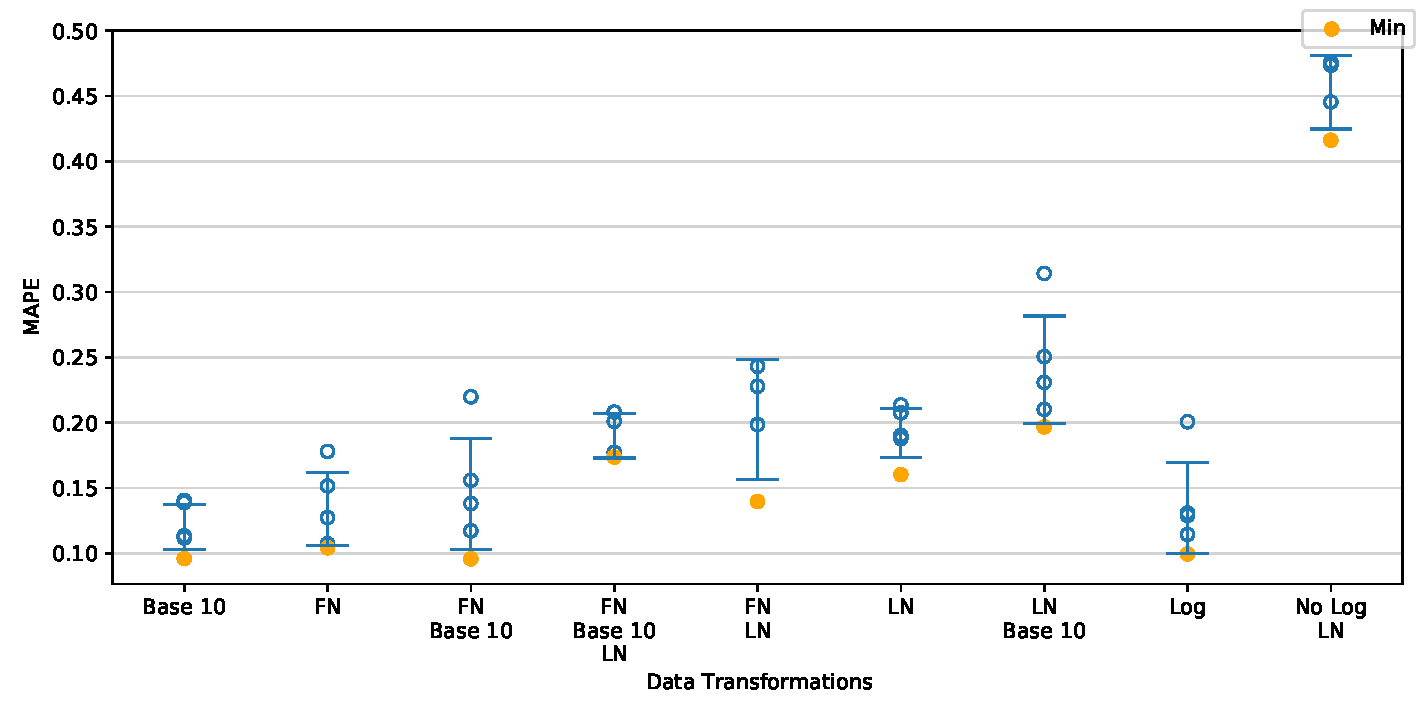
\includegraphics[width=14cm]{graphics/17,18}
	\caption{wichtig: die Daten-Transformationen ohne die überhaupt nichts geht \newline
			Base 10: Daten werden mit Logarithmus zur Basis 10 transformiert \newline
			FN: Feature-Normalization \newline
			LN: Label-Normalization \newline
			Log: Nur Scaling+Logarithmus \newline 
			No Log: Nur Scaling}
\end{figure}
\begin{figure}[tbp]
	\centering
	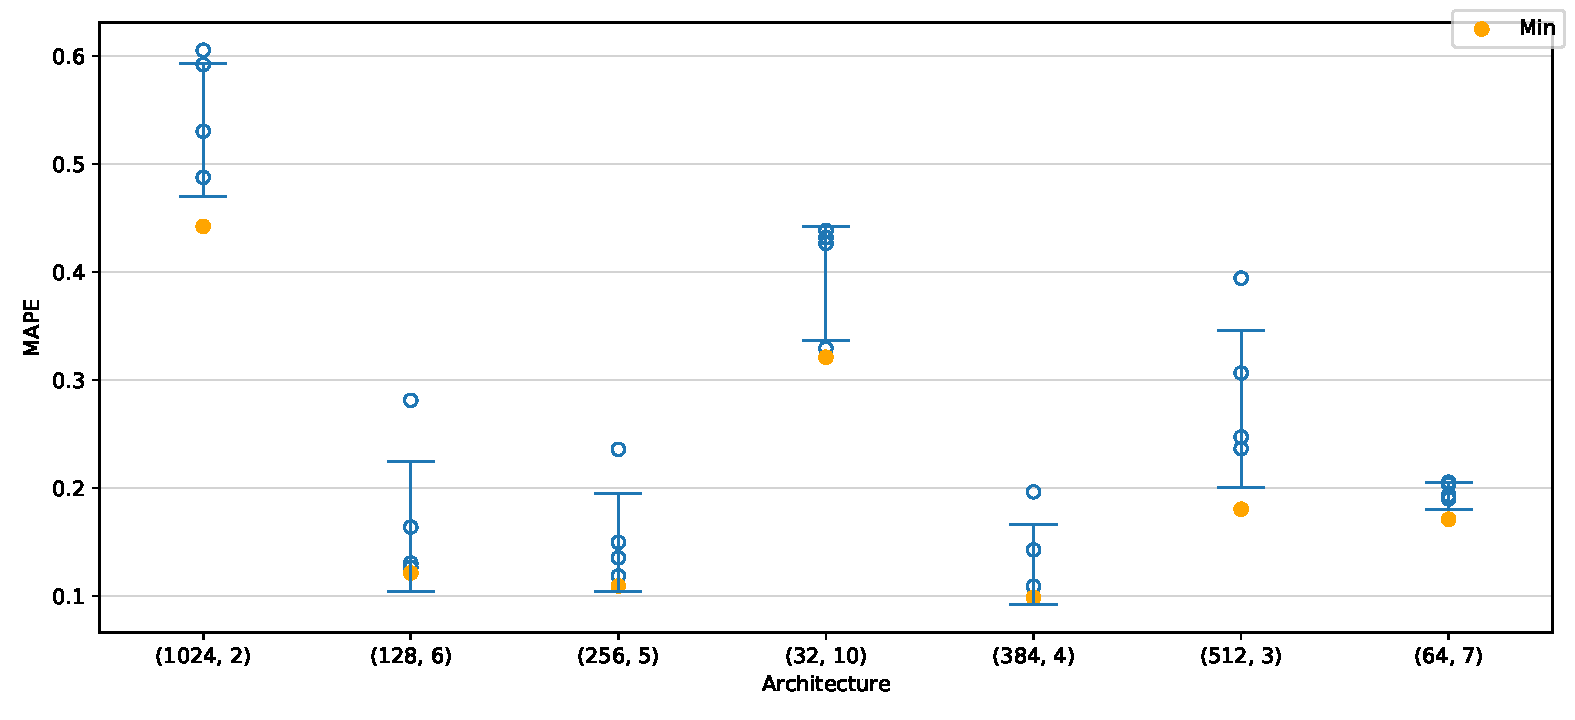
\includegraphics[width=14cm]{graphics/33}
	\caption{Vergleich für verschiedene Modell-Architekturen. \newline
		x-Labels in (Units, Nr of Layers)}
\end{figure}
\begin{figure}[tbp]
	\centering
	\subfloat[Vergleich für verschiedene Zahlen an Layern]{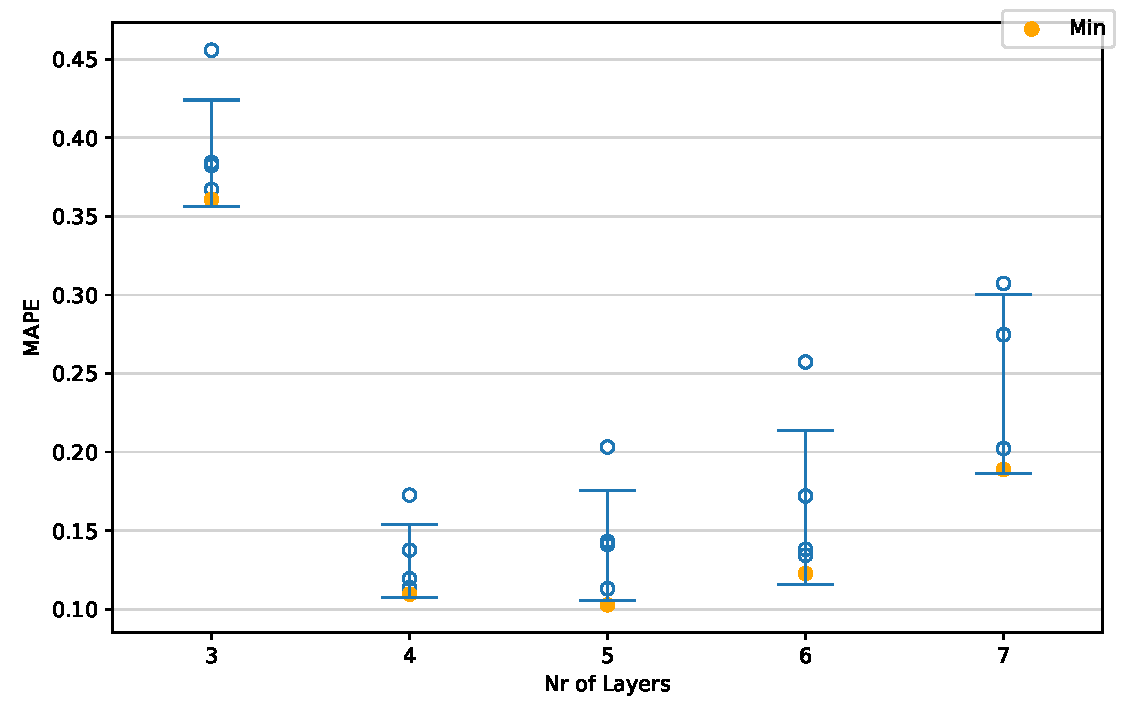
\includegraphics[width=7cm]{graphics/14}}
	\subfloat[Vergleich für verschiedene Zahlen an Units]{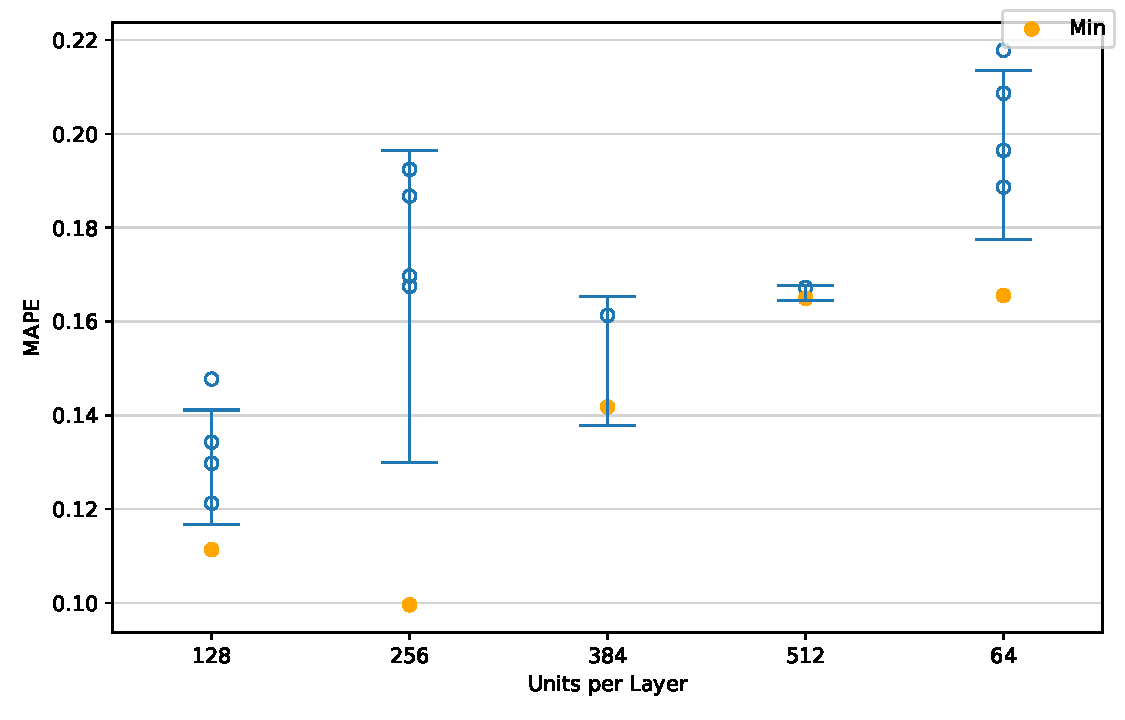
\includegraphics[width=7cm]{graphics/15}} \\
	\subfloat[Vergleich für verschiedene Activation-Functions]{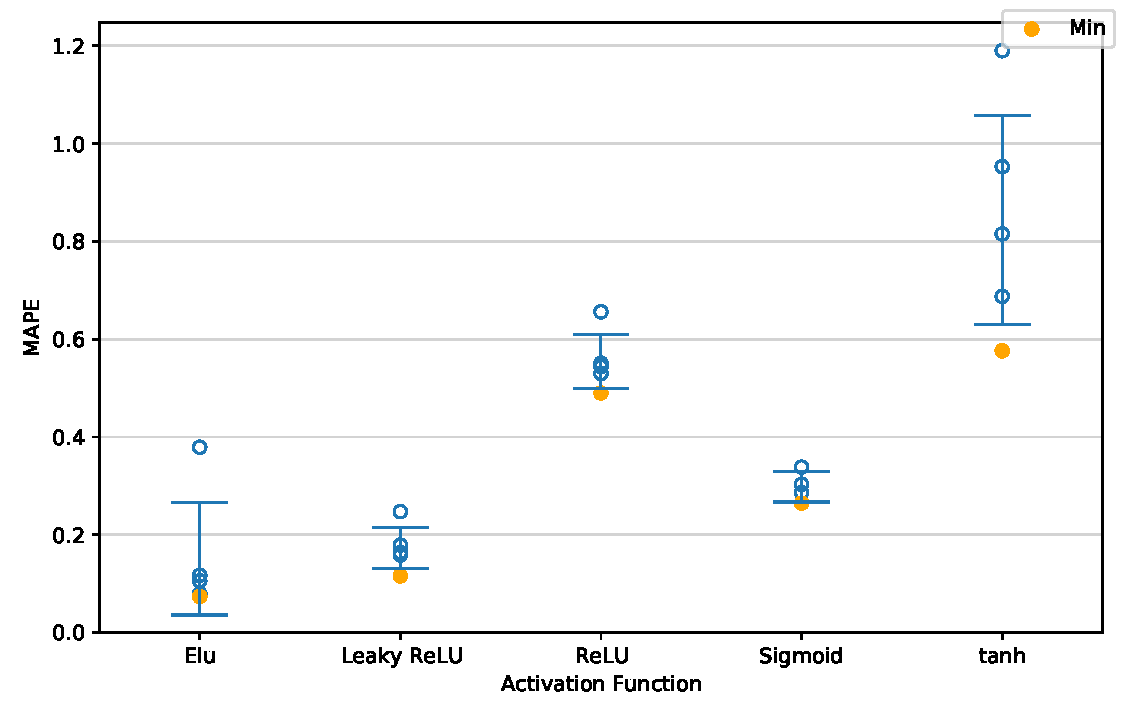
\includegraphics[width=7cm]{graphics/19}}
	\subfloat[Vergleich für verschiedene Batch-Sizes]{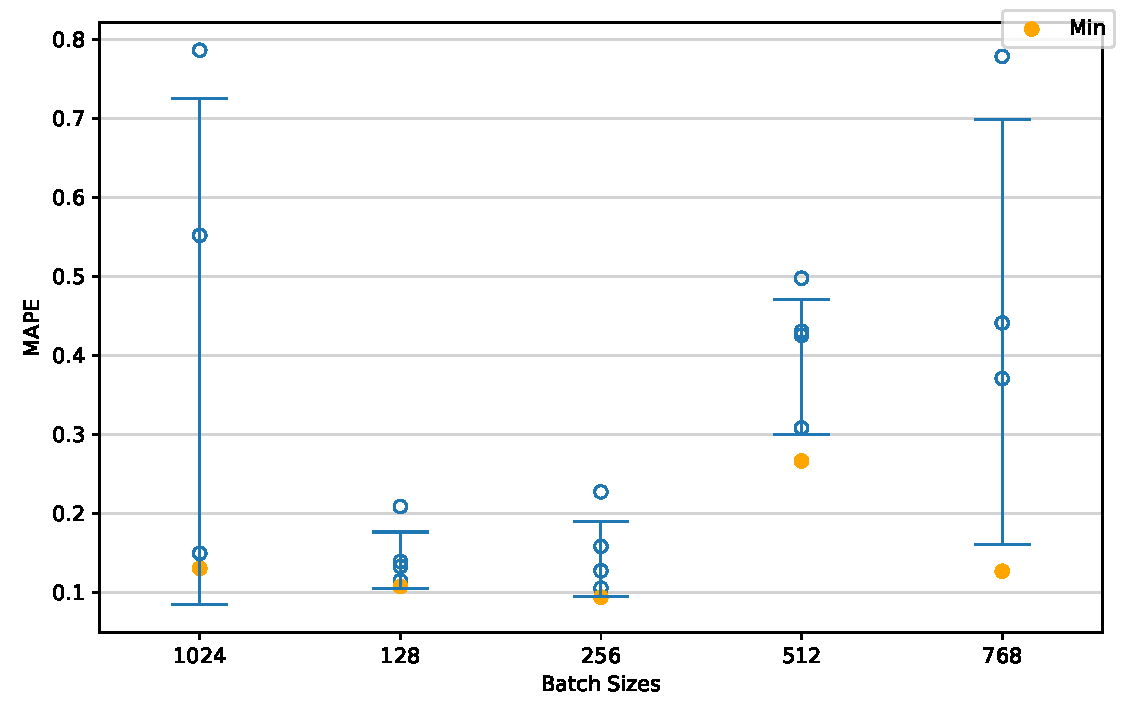
\includegraphics[width=7cm]{graphics/20}}
	\caption{Vergleich von Hyperparametern (II), MAPE: Mean-Absolute-Percentage-Error}
	\label{14,15,19,20}
\end{figure}
\section{Reweweight zwischen Fits der Partondichtefunktionen}
Eine weitere Anwendung von maschinellem Lernen, die wir besprechen wollen, ist das Reweighting von verschiedenen Anpassungen der Partondichtefunktionen. Konkret wollen wir im folgenden das Set \glqq CT14nnlo\grqq~auf \glqq MMHT2014nnlo\grqq~abbilden. Die Reweights schwanken um eins und stellen damit ein viel kleineres Problem für das Netz dar, als das vorhergegangene Modell. Auch gibt es dieses mal keine Polstellen oder Ähnliches. Für sehr hohe $x$ beginnen die Fits jedoch stark voneinander abzuweichen und die Gewicht beginnen zu oszillieren und um Größenordnungen zu fluktuieren. Es liegt daher nahe den Impulsbruchteil-Cut aus \textit{\autoref{text}} zu verwenden. Da die starken Abweichungen hier jedoch erst etwas später beginnen, entscheiden wir uns das Modell bis $x_max=0.8$ zu trainieren. \\
Der Random-Search mit den besten Parametern ist in \textit{\autoref{text}} zu sehen.

Wie erwartet, ist die Genauigkeit des Modells sehr gut, wie wir in \textit{\autoref{text}} beobachten können. Die Abweichung beträgt generell weniger als $0.1\%$ und ist somit praktisch kaum von den analytisch berechneten Werten zu unterscheiden. Wie das gelernte Reweight in der Praxis funktioniert, ist in \textit{\autoref{text}} dargestellt. Auch hier können wir nur minimale Abweichungen verzeichnen. Wir betrachten nur kleine Bereiche in $x$, um den Unterschied zwischen den PDF-Sets aufzulösen. Das Ratio in \textit{\autoref{text}} c) ist wie erwartet konstant, da das Reweight nicht von $\eta$ abhängt (siehe \textit{\autoref{text}}). 
\begin{figure}[tbp]
	\centering
	\subfloat[Schnitt in $x_1$]{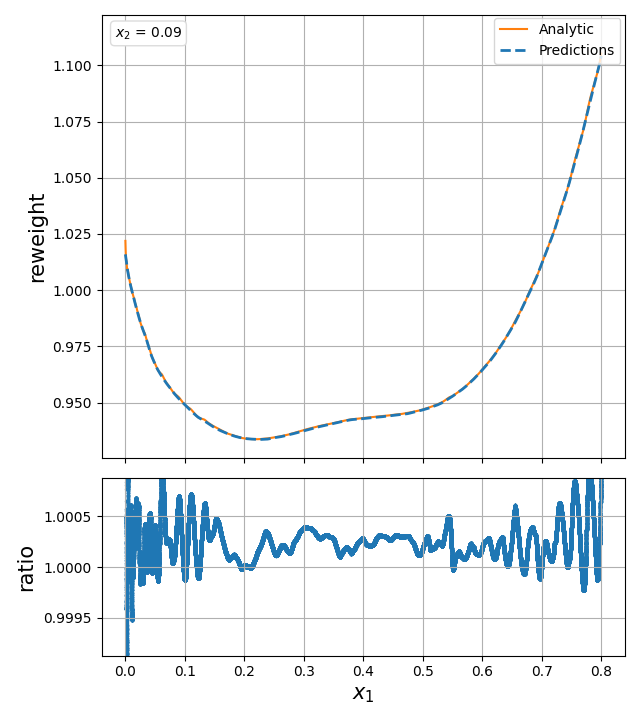
\includegraphics[width=7cm]{graphics/32}}
	\subfloat[Schnitt in $x_2$]{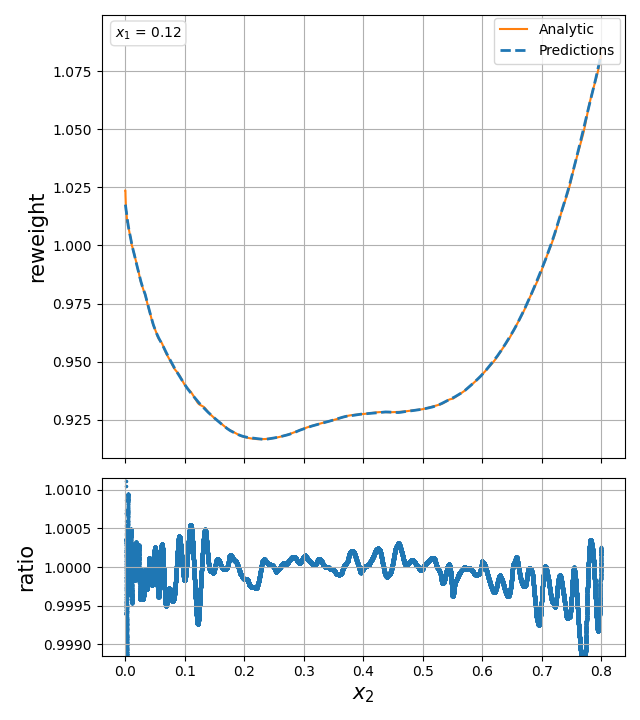
\includegraphics[width=7cm]{graphics/33_1}} 
	\caption{Vlt noch 2 3D-plots, einmal die analytischen Reweights, gelernte Reweights werden aber gleich aussehen bei der geringen abweichung}
	\label{32,33}
\end{figure}
\begin{figure}[tbp]
	\centering
	\subfloat[Schnitt in $x_1$]{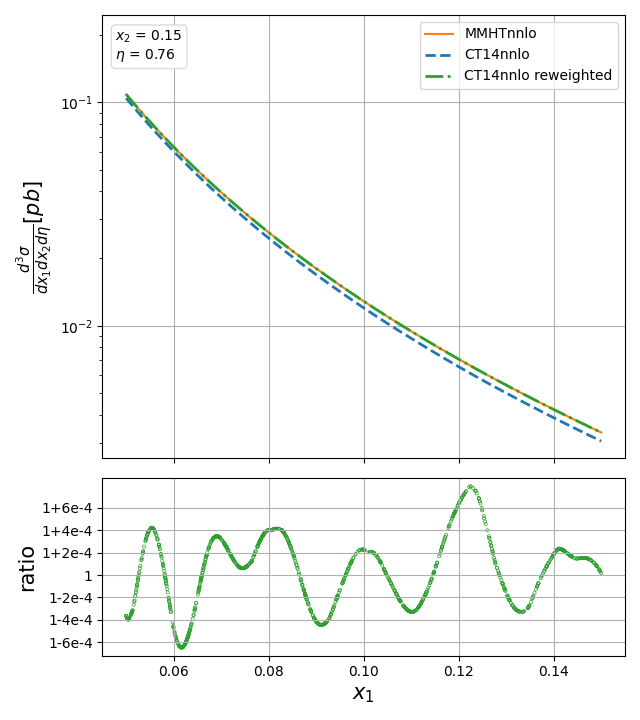
\includegraphics[width=7cm]{graphics/22.0}} 
	\subfloat[Schnitt in $x_2$]{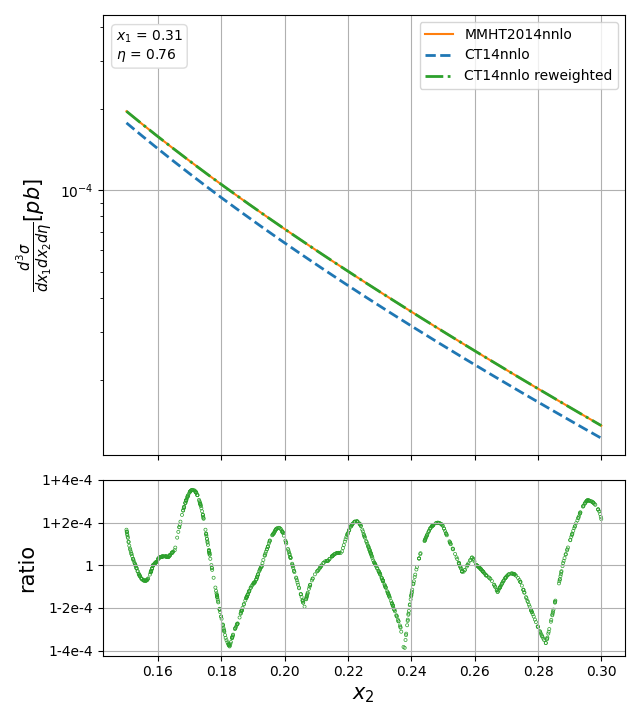
\includegraphics[width=7cm]{graphics/23.1}} \\
	\subfloat[Schnitt in $\eta$]{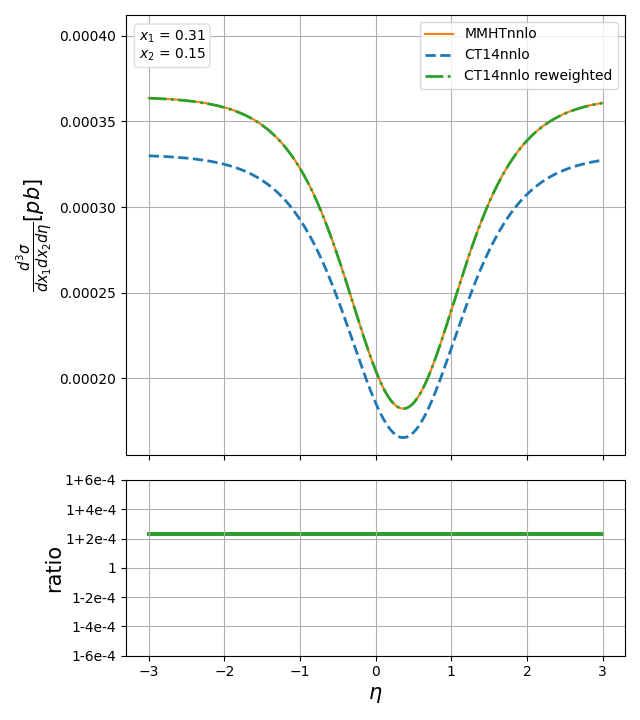
\includegraphics[width=7cm]{graphics/21.0}}
	\caption{Reweight von CT14nnlo auf MMHT2014nnlo mittels gelernten Weigths}
	\label{21,22,23}
\end{figure}
\section{Transfer-Learning zwischen verschiedenen Fits der Partondichtefunktionen}
Eine weitere Möglichkeit, den Wirkungsquerschnitt, der mit einem anderen PDF-Set berechnet wurde, zu erhalten, ist Transfer-Learning. Wie wir gesehen haben, unterscheiden sich die Wirkungsquerschnitte von den verschiedenen Fits in den relevanten Phasenraumbereichen nur minimal. Mit Transfer-Learning können wir diesen Unterschied ausgleichen und mit wenig Aufwand gut Modelle für andere PDF-Fits erhalten. Das Grundprinzip von Transfer-Learning ist bereits in \textit{\autoref{??}} festgehalten. Wir nutzen wieder einen Random-Search, um gute Hyperparameter für den Transfer zu finden. Diese können in \textit{\autoref{label}} nachgelesen werden.\\

In \textit{\autoref{label}} sind Schnitte des differentiellen Wirkungsquerschnitts mit transferiertem Modell, dem Modell das als Quelle gedient hat, und den analytischen Werten gezeigt. Wir können beobachten, dass die Genauigkeit des transferierten Modells fast identisch mit der des Source-Modells in \textit{\autoref{text}} ist. Das Modell verliert also beim Transfer nicht signifikant an Genauigkeit. Wir beobachten jedoch auch keine Verbesserung der Performance, was dem Transfer-Learning manchmal zugesprochen wird. Interessant zu sehen ist, dass sich die Form des Ratios beider Modell in \textit{\autoref{label}} ähnelt. Der Grund hierfür liegt darin, dass das transferierte Modell vom Source-Modell abstammt.\\
Eindeutig können wir sehen, dass sich die Menge an Trainigsdaten und damit auch die Trainingsdauer stark verringert. Es konnte mit einfachen Mitteln eine Reduktion um den Faktor vier an Trainingsdaten erreicht werden. Automatisch verkürzt sich hiermit auch die Trainingszeit, wie in \textit{\autoref{text}} aufgeführt ist. 
Sowohl das Transfer-Learning, als auch das Reweighting sind also legitime Methoden um den Wirkungsquerschnitt von einem PDF-Set auf das nächste zu übertragen. Es stellt sich nun die Frage, welche Methode besser geeignet ist und wo jede Methode seine stärken und Schwächen hat. Zunächst sind in \textit{\autoref{text}} noch einmal Schnitte des Wirkungsquerschnitts gezeigt. In den Ratios lässt sich ?vermuten?, dass das neu gewichtete Source-Model etwas bessere Vorhersagen trifft. \\
\newline
In \textit{\autoref{text}} sind einige Eigenschaften gegenübergestellt.
\begin{table} % TODO Trainingszeit passt noch nicht so ganz
	\centering
	\begin{tabular}{|l|c|c|c|c|}
		\hline
		Modell & MAPE & Training$[\text{s}]$ & Punkte & TPM$[\text{s}]$ \\
		\hline
		Reweight + Source & 0.076 & 243.42 & 1M & 30.60 \\
		Reweight + Analy. &  0.017 & 243.42 & 1M & 13.84 \\
		Transfer & 0.204 & 85.78 & 1M & 15.73\\
		Transfer + FT & 0.064 & 164.83 & 1M & 15.65 \\
		Source-Model & 0.229 & 841.46 & 4M & 15.81\\
		\hline
	\end{tabular}
	\caption{Vergleich von Reweight- und Transfer-Modellen \newline TPM: Time per Million, Berechnungszeit für $10^{6}$ Punkte}
\end{table}
Wir sehen, dass das präziseste und schnellste Modell das Reweighting der analytisch berechneten Werte ist. Verfügt man also bereits über eine große Anzahl an Werten von differentiellen Wirkungsquerschnitten, dann ist dies das Modell der Wahl. Möchten wir jedoch über ein vollständiges Modell verfügen, dass nicht auf die analytische Berechnung von differentiellen Wirkungsquerschnitten angewiesen ist, fällt diese Möglichkeit jedoch heraus. Hier schneidet das Modell \glqq Transfer + FT\grqq~am Besten ab. Es sticht seinen Konkurrenten \glqq Reweight + Source\grqq~ in allen betrachtet Kriterien aus. Da im zweiten Fall sowohl die Reweights mit einem Netz, als auch die Source-Wirkungsquerschnitten mit neuronalen Netzen berechnet werden, verdoppelt sich hier die TPM im Vergleich zu den restlichen Modellen. Während das Transfer+FT ein neues Modell ergibt, dass für das neue PDF-Set ebenso gut funktioniert wie das Souce-Modell am vorherigen Set, bleibt der MAPE in etwa konstant. Gewichten wir jedoch die Ergebnisse des Source-Model neu, pflanzen sich beide Ungenauigkeiten fort und die Unsicherheit steigt etwas. In \textit{\autoref{text}} ist noch einmal die Performance der angesprochenen Modelle miteinander verglichen.\\
\newline
Wir kommen zum Schluss, dass das Transfer-Learning eine generell bessere Methode für den angesprochenen Zweck ist und das Erlernen des Reweights zwar gut funktioniert, jedoch nur nützlich ist, wenn man für speziell die Gewichte benötigt.
\subsection{...}
\begin{figure}[tbp]
	\centering
	\subfloat[Schnitt in $x_1$]{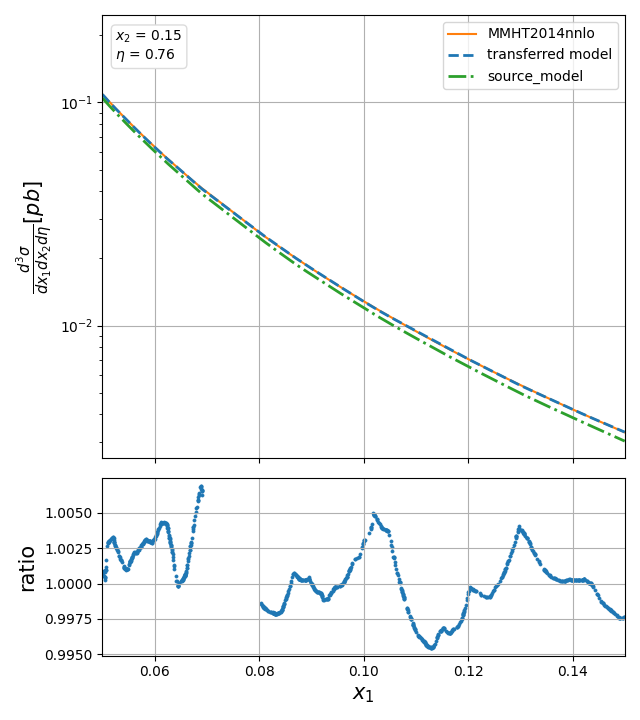
\includegraphics[width=7cm]{graphics/34.0}} 
	\subfloat[Schnitt in $x_2$]{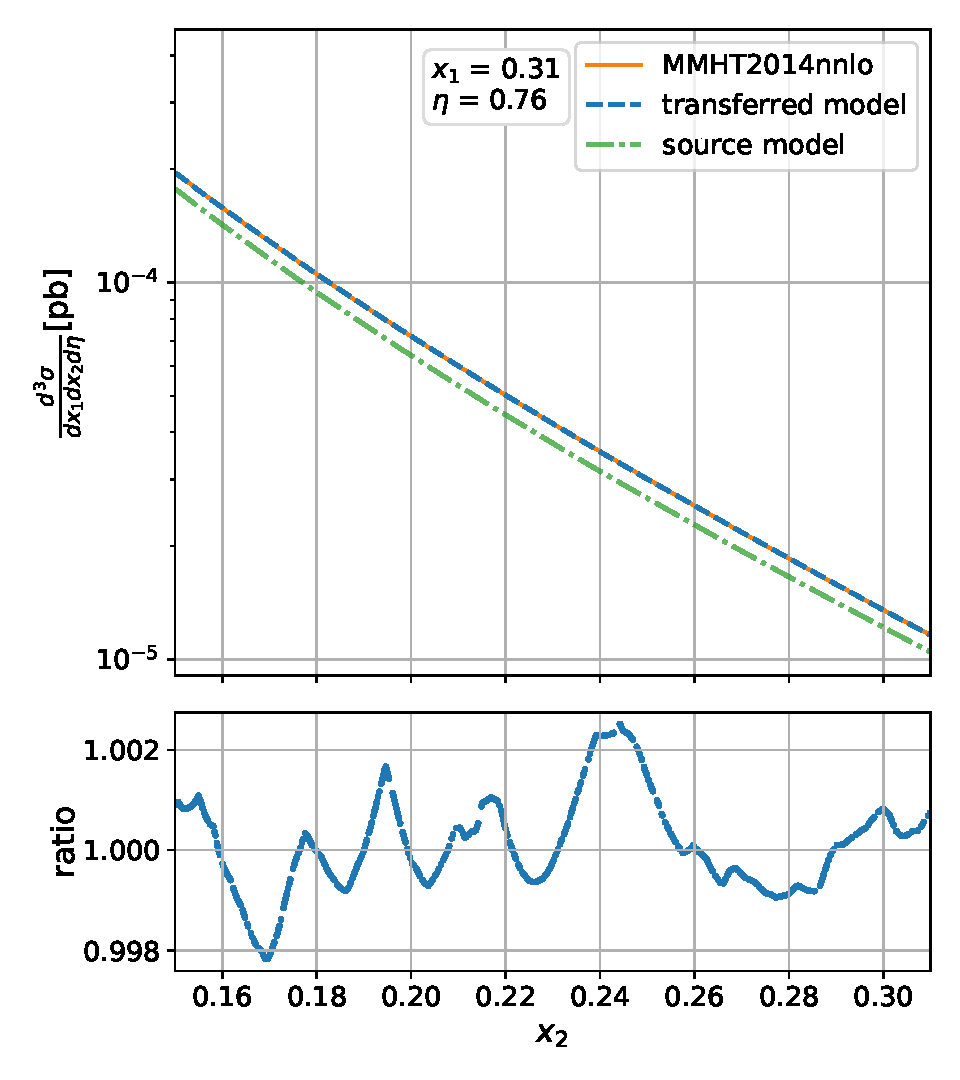
\includegraphics[width=7cm]{graphics/35.1}} \\
	\subfloat[Schnitt in $\eta$]{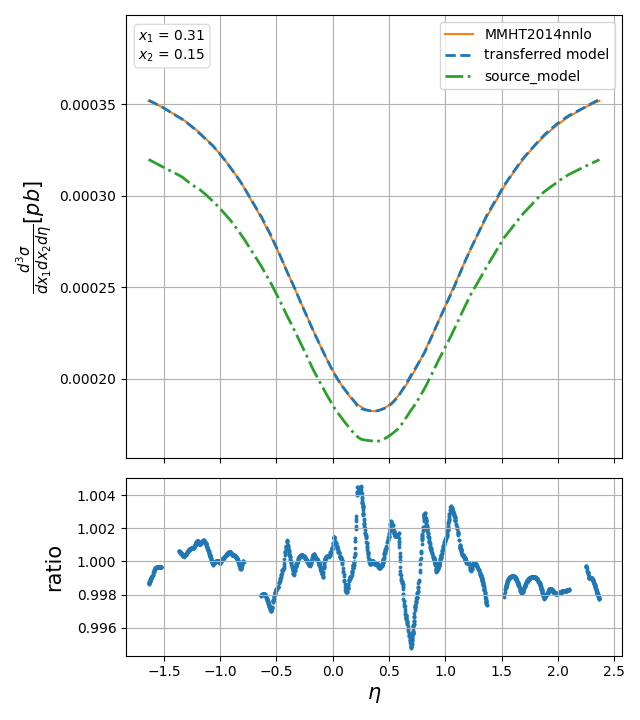
\includegraphics[width=7cm]{graphics/24}}
	\caption{Transferiertes Model von Source Model zum Transfer model}
	\label{34,35,24}
\end{figure}

\begin{figure}[tbp]
	\centering
	\subfloat[Schnitt in $x_1$]{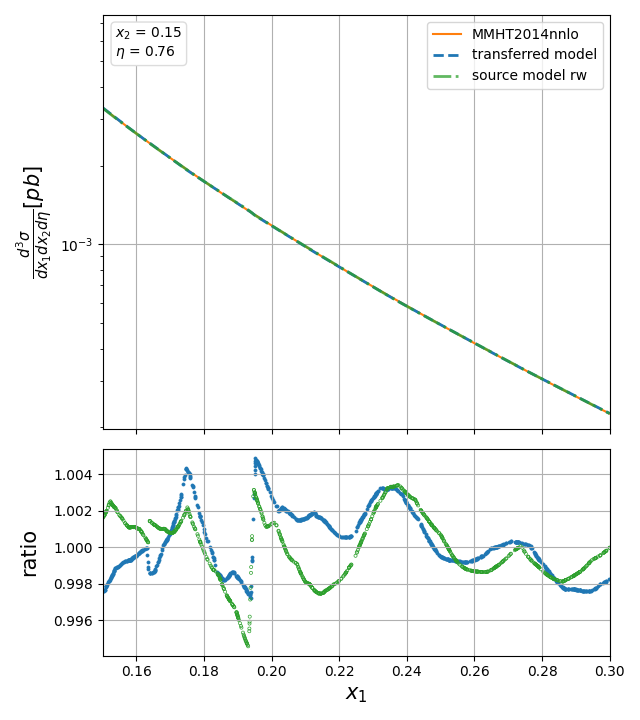
\includegraphics[width=7cm]{graphics/34.2}} 
	\subfloat[Schnitt in $x_2$]{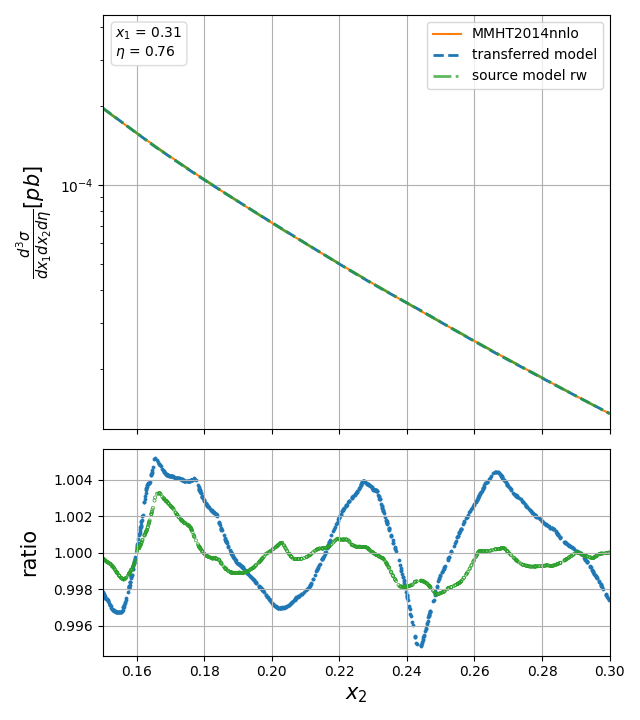
\includegraphics[width=7cm]{graphics/35.2}} \\
	\subfloat[Schnitt in $\eta$]{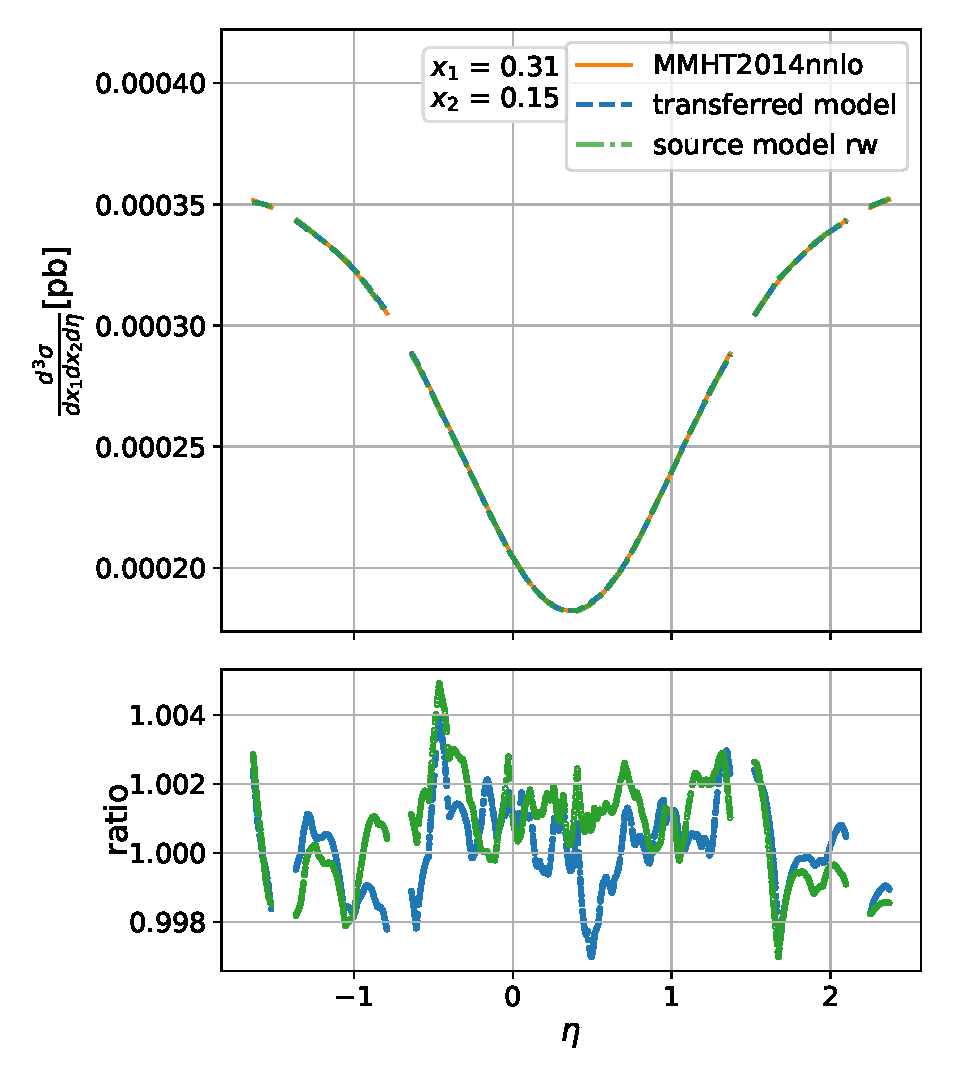
\includegraphics[width=7cm]{graphics/24.2}}
	\caption{Vergleich transferiertes Modell, gereweightetes Source Model \newline
		rw: reweighted}
	\label{34,35,24,reweight}
\end{figure}
\begin{figure}
	\centering
	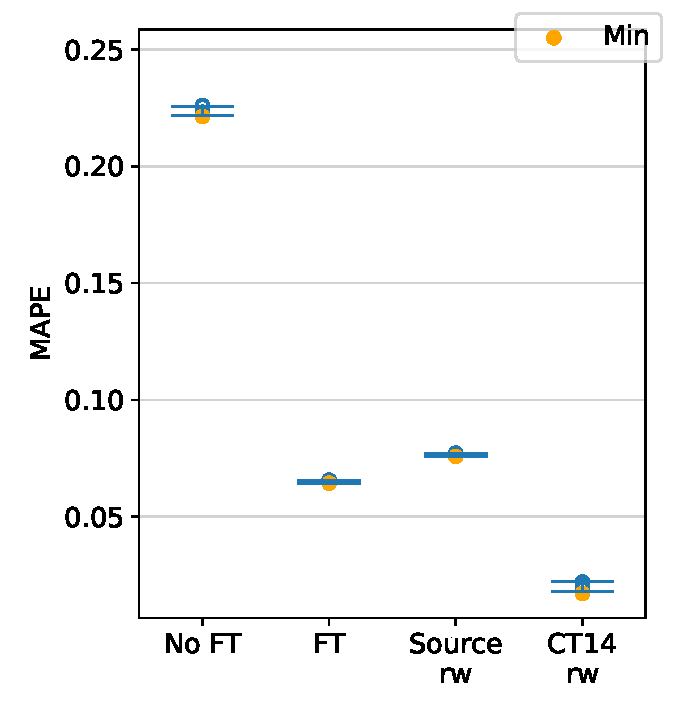
\includegraphics[width=6cm]{graphics/25,29}
	\caption{Vergleich von Transfer Learning mit und ohne Fine-Tuning, Vergleich mit gereweithenem source model kommt noch}
\end{figure}
\section{Monte-Carlo-Integration}
\subsection{Partonischer Wirkungsquerschnitt}
Wir nutzen Monte-Carlo-Methoden zur Integration von \textit{\autoref{text}}, \textit{\autoref{text}} und deren zugehörigen Machine Learning Modellen. Zur Integration von \textit{\autoref{text}} nutzen wir das Importance Sampling aus \textit{\autoref{text}}, um die Konvergenz des Integrals zu beschleunigen. Der Prozess $qq \rightarrow \gamma \gamma$ ist zwar nicht messbar, jedoch müssen wir trotzdem einen Cut in $\eta$ festlegen, da der totale Wirkungsquerschnitt sonst divergiert. Wir entscheiden uns für die Beschränkungen \textit{\autoref{text}}.
\begin{equation}
	\abs{\eta} \leq 2.5 \qquad \Rightarrow \qquad \theta \in \left[\epsilon, \pi - \epsilon \right] \quad \text{mit} \quad \epsilon = 0.1638
\end{equation}
Die Unsicherheit auf unsere Monte-Carlo-Integration bestimmen wir aus \textit{\autoref{text}}. Wir führen die Integrationen mit 1000 Stützstellen durch und wiederholen die Integration 100 mal. In \textit{\autoref{text}} sind die erhaltenen Ergebnisse mit dem analytischen Wert verglichen.
\begin{table}
	\centering
	\begin{tabular}{lll}
		Integrand & \multicolumn{2}{c}{$\quad \sigma_{\text{tot}}[\text{pb}]$} \\
		\hline
		analytische Integration& \quad  $0.053793$ &$\pm~ 0$\\
		$\derivative{\sigma}{\theta}$ analytisch + IS & $\quad 0.05382 $&$\pm~ 0.00006 $ \\
		$\derivative{\sigma}{\theta}$ analytisch & $\quad 0.05389$ &$\pm~ 0.00015 $ \\
		$\derivative{\sigma}{\theta}$ ml + IS &$\quad 0.05386$ &$\pm~ 0.00005$ \\
		$\derivative{\sigma}{\eta}$ analytisch & $\quad 0.053796 $&$\pm~ 0.000034$ \\
		$\derivative{\sigma}{\eta}$ ml & $\quad 0.053801 $&$\pm~ 0.000034$ \\
	\end{tabular}
	\caption{Monte-Carlo-Integration des partonischen Diphoton Prozesses}
\end{table}
Wir sehen, dass die neuronalen Netze so präzise sind, dass ihre Abweichung in de Monte-Carlo-Integration untergeht. Das sind gute Voraussetzungen für die Anwendbarkeit von neuronalen Netzen auch bei höherdimensionalen Prozessen. Das simple Importance-Sampling bringt eine signifikante Varianz-Verringerung mit sich.
\subsection{Hadronischer Diphoton-Prozess}
 Auch für den hadronischen Diphoton-Prozess nutzen wir Importance-Sampling. Für die Generation der Impulsbruchteile $x$ verwenden wir die Verteilung aus \textit{\autoref{text}}. Aufgrund der Cuts leisten Phasenraumpunkte mit kleinem $\eta$ einen Größeren Beitrag zum messbaren $\sigma_{\text{tot}}$, wir ziehen daher Punkte aus einer Gaußverteilung um Null($\textit{\autoref{label}}$).
 \begin{equation}
 		\rho(\eta) = \frac{1}{\sqrt{2\pi \sigma^2}} \exp(-\frac{(\eta)^2}{2\sigma^2}) \quad \text{mit} \quad \sigma=2
 \end{equation}
 Wir integrieren zunächst über zwei Freiheitsgrade und sehen uns die Wirkungsquerschnitte in Abhängigkeit von $x_1, x_2$ und $\eta$ an. Wir samplen dazu 50.000.000 Punkte, mit gleicher Sample-Effizienz wie in \textit{\autoref{label}} und wiederholen den Prozess fünf mal. Die Ergebnisse sind in \textit{\autoref{label}} dargestellt.
\begin{figure}[tbp]
	\centering
	\subfloat[]{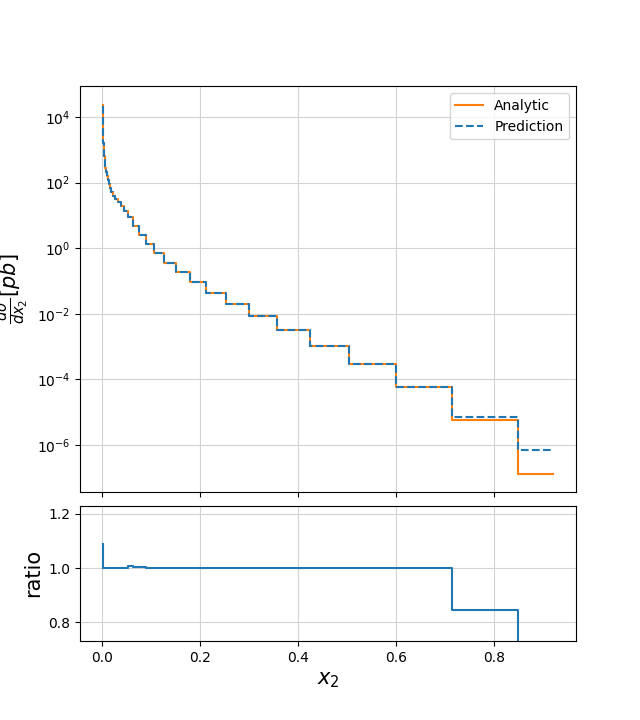
\includegraphics[width=7cm]{graphics/27}} 
	\subfloat[]{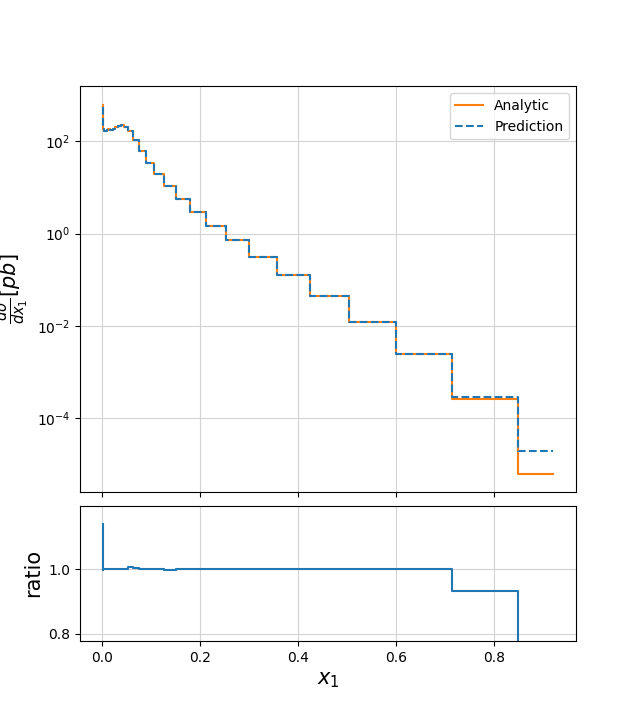
\includegraphics[width=7cm]{graphics/28}} \\
	\subfloat[]{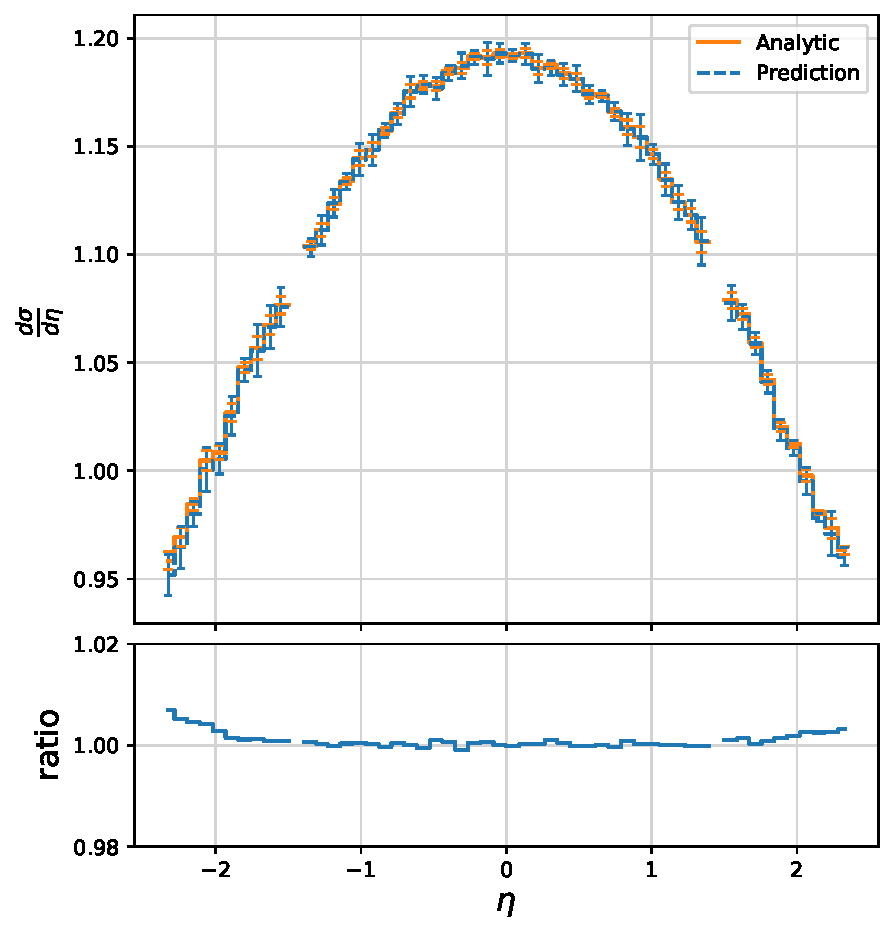
\includegraphics[width=7cm]{graphics/11}}
	\caption{MC-Integrationen über zwei Freiheitsgrade}
	\label{11,27,28}
\end{figure} %TODO sicherstellen, dass ratio immer analytisch/WQ ist.
Wie wir sehen, überdecken sich die integrieren Wirkungsquerschnitte für die analytischen Werte und die Vorhersagen des neuronalen Netzes an vielen Phasenpunkten. Lediglich für große $x$ überschätzt die Vorhersage wie erwartet den eigentlichen Wert. Dass die Auswirkungen dieser Überschätzung jedoch eindeutig zu vernachlässigen sind, kann schon in Teil c) von \textit{\autoref{label}} beobachtet werden. Das Ratio ist bis auf wenige Ausnahmen größer als eins, was bedeutet, dass unsere Vorhersagen zu klein sind. Der Grund hierfür liegt vermutlich in der Polstelle an $x=0$. Durch die Cuts werden viele Phasenraumpunkte mit großem Wirkungsquerschnitt herausgenommen, da sie die $p_T$-Hürde nicht erfüllen. Dem Netz unterschätzt dadurch generell diese Punkte und in den Monte-Carlo-Integration kommt es dann dazu, dass wenige Punkte generiert werden, die große Einflüsse auf den integrierten Wirkungsquerschnitt haben. Die Unterschätzung dieser Punkte ist dann viel gravierender, als die Überschätzung in Phasenraumbereichen mit hohen $x$. \\
\newline
Zur Integration über alle Freiheitsgrade verwenden wir die gleichen Daten wie im vorherigen Abschnitt. Wir erhalten die Ergebnisse \textit{\autoref{label}}.
\begin{equation}
	\begin{split}
	\sigma_{tot}^{analytic} =  5.1707 \pm 0.0038 \\
	\sigma_{tot}^{prediction} = 5.1634 \pm 0.0038 \\
	\end{split}
\end{equation}
\begin{table}
	\centering
	\begin{tabular}{lll}
		Integrand & \multicolumn{2}{l}{$\quad \sigma_{tot}$[pb]} \\
		\hline
		analytic & & \\
		prediction & & \\
	\end{tabular}
\end{table}
\chapter{Zusammenfassung und Ausblick}
\section{Zusammenfassung}
In dieser Arbeit wurde der Diphoton Prozess als $q\overline{q} \rightarrow \gamma \gamma$ und $pp \rightarrow \gamma \gamma$ auf Leading-Order Ebene behandelt und Ausdrücke für die jeweiligen differentiellen Wirkungsquerschnitte hergeleitet. An dies Beispielen wurde dann die Eignung von tiefen neuronalen Netzwerken zur Näherung des Integranden überprüft. Dabei mussten verschiedene Tücken bedacht und behandelt werden. In diesem Kontext wurde die Wichtigkeit von Label-Transformationen und der Architektur des Neuronalen Netzes deutlich. Anschließend wurden die Gewichte zwischen den Fits der Partondichtefunktionen CT14nnlo und MMHT2014nnlo erlernt und angewendet. Schließlich wurde noch die Möglichkeit des Transfer-Learning zwischen Modellen, die an verschiedenen PDF-Sets trainiert wurden überprüft. Mithilfe von Monte-Carlo-Methoden wurden die differentiellen Wirkungsquerschnitte integriert.

Wir erwartet, haben die neuronalen Netze keine Probleme mit simplen Regressionsaufgaben, wie die Wirkungsquerschnitte des Prozesses $q\overline{q} \rightarrow \gamma \gamma$ darstellen. Die Funktionswerte können mit ausgezeichneter Genauigkeit und wenig Aufwand vorhergesagt werden.\\
Andererseits ist der differentielle Wirkungsquerschnitt des Prozesses $pp \rightarrow \gamma \gamma$ wiederum nicht trivial. Hier müssen Hürden wie das \glqq Dying-ReLU\grqq~Problem und die passende Wahl der Loss-Function beachtet werden. Auch kann es hier helfen kaum beitragende Phasenraumbereiche zu vernachlässigen, um die Spanne an Größenordunungen, über die sich die Wirkungsquerschnitte verteilen, zu verkleinern. Letztendlich kann mit etwas Feingefühl und Erfahrung im Umgang mit neuronalen Netzen jedoch passende Modelle gefunden werden, die gute Genauigkeit zeigen.\\
Das Erlernen der Reweights stellt aus Sicht des neuronalen Netzes kein Problem dar, solange ein sinnvoller Phasenraumbereich gewählt wird. Hier kann das Netz die Funktionswerte mit exzellenter Genauigkeit vorhersagen. Das neuronale Netz kann also hier gut als Interpolation zwischen den analytischen Werten dienen. \\
Transfer-Learning stellt sich als eine gute Möglichkeit heraus, aus einem bereits vorhandenen Modell, ein Modell für einen anderen Fit von Partondichtefunktionen zu erhalten. In puncto Berechnungs- und Trainingsgeschwindigkeit und Genauigkeit übertrifft das Transfer-Learning hier das Reweighten eines bereits vorhandenen Source-Models.

\section{Ausblick}
Die in dieser Arbeit behandelten Methoden haben gute Ergebnisse an den einfachen Beispielen gezeigt. Als nächstes sollte nun der Test an höherdimensionalen Prozessen mit analytisch nicht mehr oder nur aufwändig zu berechnenden Wirkungsquerschnitten folgen. Es muss noch untersucht werden, ob die neuronalen Netze ihre Genauigkeit auch in höheren Dimensionen aufrechterhalten können und wenn ja, ob dies mit einer realistischen Zahl an Trainingspunkten möglich ist. Anschließend muss überprüft werden, wie groß der rechentechnische Nutzen der neuronalen Netze. In den einfachen, analytischen Beispielen von uns ist der analytische Weg noch um einen Faktor zwei schneller. Die in dieser Arbeit erhaltenen Ergebnisse sind jedoch gute Voraussetzungen für die Funktionstüchtigkeit im Höherdimensionalen. Zusätzlich sind neuronale Netze dafür bekannt mit sehr hochdimensionalen Eingangswerten umgehen zu können. \\
\newline
Auch das Transfer-Learning hat in dieser Arbeit seine Funktionalität bewiesen. Es muss jedoch nicht beim Transfer zwischen PDF-Sets bleiben. In der Praxis wird Transfer-Learning zwischen viel diverseren Datensets eingesetzt. Es könnte sich also lohnen, auch den Transfer zwischen sich ähnelnden Prozessen in der Teilchenphysik zu untersuchen. Ich spreche hier von Vorgängen die sich beispielsweise nur durch das Vorhandensein von Myonen anstatt Elektronen unterscheiden oder auch den Transfer von Leading-Order Prozessen zu höheren Ordnungen. \\
\newline
Abgesehen von den hier untersuchten Verwendungsmöglichkeiten gibt es noch unzählige weiter Anwendungsmöglichkeiten von Machine-Learning oder tiefen neuronalen Netzen in der Teilchenphysik. Hierunter fällt beispielsweise... 

%TODO Transfer zwischen ähnlichen Prozessen, nicht nur PDF-Sets 
%TODO Schwerpunktsenergie die du verwendet hast festschreiben
 

\appendix
\chapter{Anhang}
\begin{figure}[tbp]
	\centering
	\subfloat[Rectified Linear Unit: $f(x) = \text{max}(0, x)$]{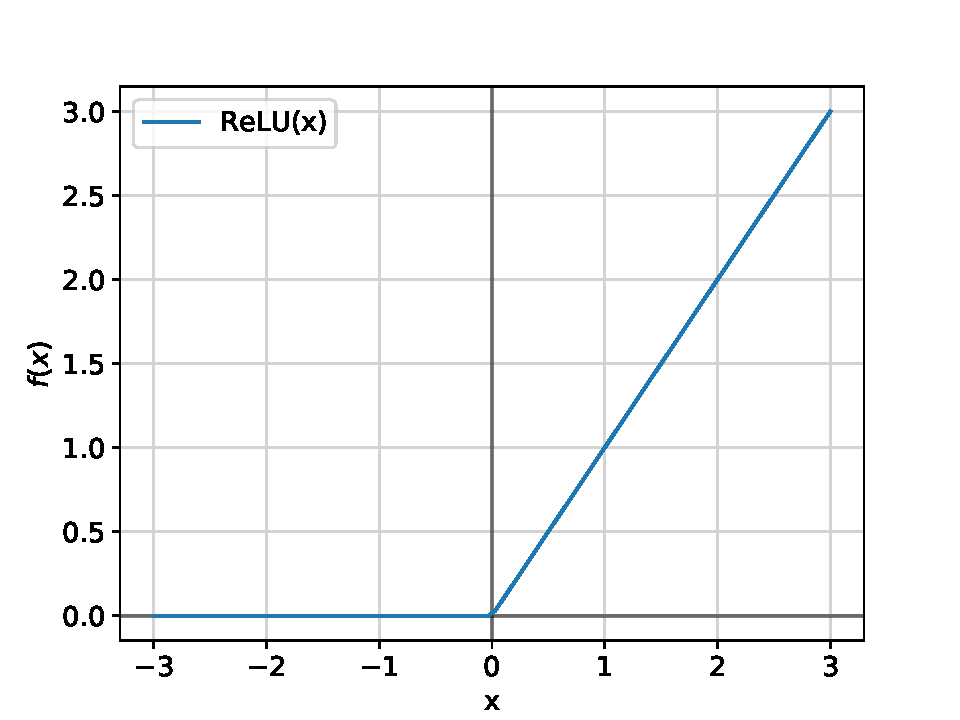
\includegraphics[width=7cm]{graphics/ReLU(x)}} 
	\subfloat[Leaky-ReLU: $f(\alpha, x) = \alpha x$ für $x<0$]{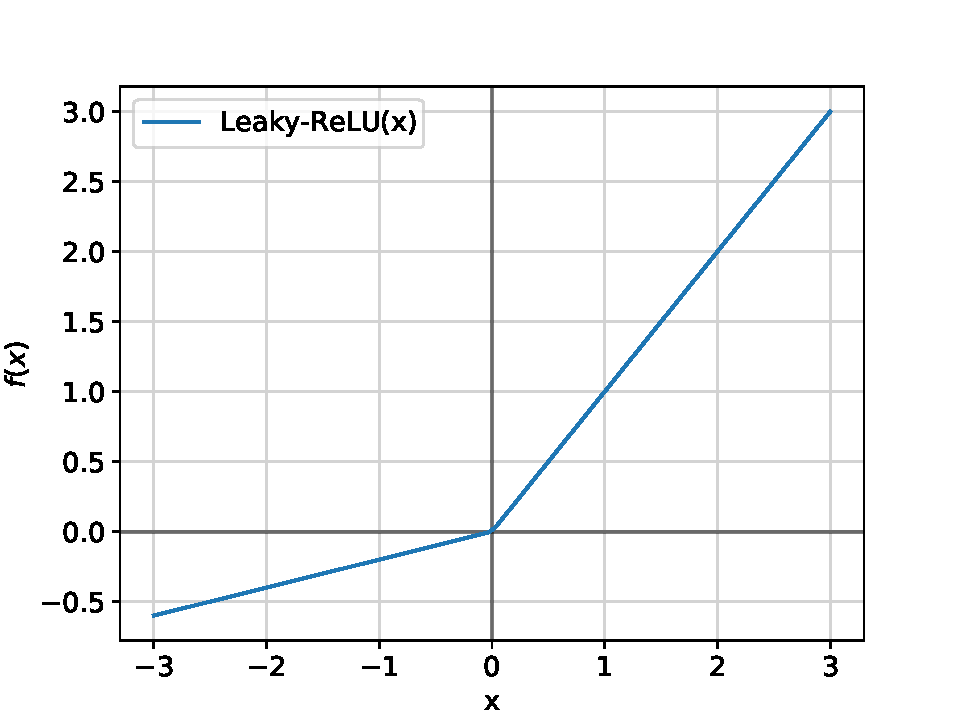
\includegraphics[width=7cm]{graphics/Leaky-ReLU(x)}} \\
	\subfloat[ELU: $f(\alpha, x) = \alpha(e^x - 1)$ für $x < 0$]{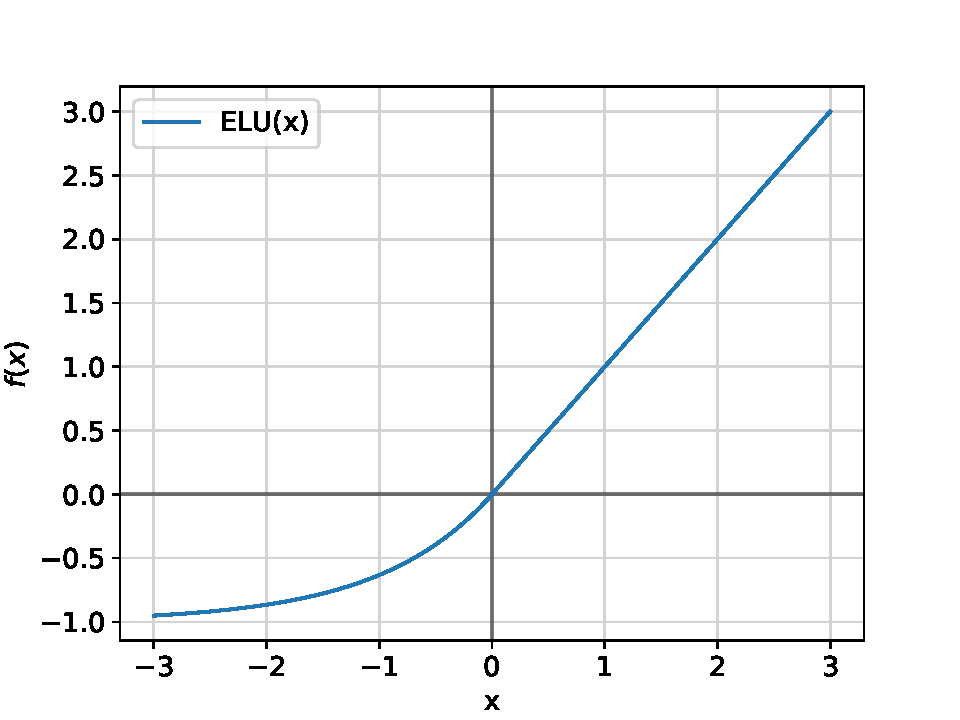
\includegraphics[width=7cm]{graphics/ELU(x)}}
	\subfloat[Sigmoid: $f(x) = \frac{e^x}{e^x + 1}$]{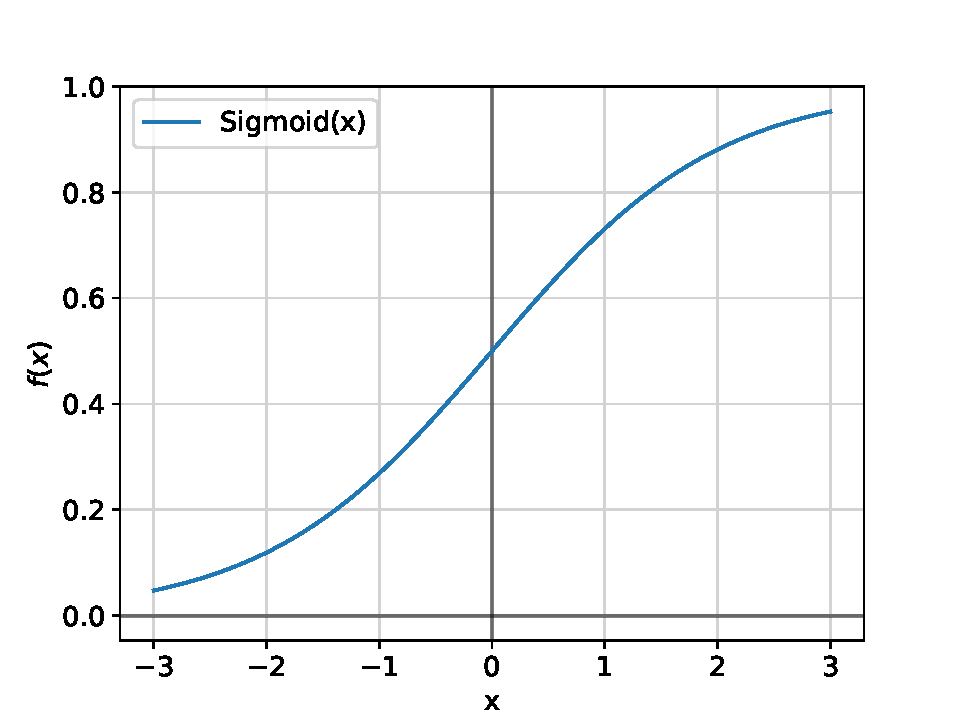
\includegraphics[width=7cm]{graphics/Sigmoid(x)}} \\
	\subfloat[tanh : $f(x) = tanh(x)$]{\includegraphics[width=7cm]{graphics/tanh(x)}}
	\subfloat[Exp: $f(x) = e^x$]{\includegraphics[width=7cm]{graphics/Exp(x)}} \\  
	\caption{Activation-Funkctions, die verwendet wurden}
	\label{11,27,28}
\end{figure}
\begin{table}
	\centering
	\begin{tabular}{|l|l|l|}
		\hline
		Hyperparameter & Pool & Best Config \\
		\hline
		Anzahl Layer & $\left\lbrace 1, 2, 3, 4 \right\rbrace$ & 4 \\
		Anzahl Units & $\left\lbrace 32, 64, 128, 256\right\rbrace$ & 128 \\
		Loss-Funktion & MAE, MSE, Huber & MAE \\
		Optimizer & Adam, RMSprop, SGD  & Adam\\
		Aktivierungsfunktion & ReLU, Leaky-ReLU, Sigmoid & Leaky-ReLU \\
		Learning-rate & $\left\lbrace 10^{-2}, 5 \cdot 10^{-3}, 10^{-3}, 10^{-4} \right\rbrace $ & $5 \cdot 10^{-3}$\\
		Batch-Größe & $\left\lbrace 64, 128, 512, 768, 2048 \right\rbrace $ & 128\\
		Label-Normalisierung & $\left\lbrace \text{keine}, [-1,1]\right\rbrace $ & $[-1,1]$\\
		\hline
		Max. Epochen & \multicolumn{2}{c|}{200}\\
		Anzahl Trainingspunkte & \multicolumn{2}{c|}{60000} \\
		\hline
	\end{tabular}
	\caption{Parameter der Random-Search für $\frac{d\sigma}{d\theta}$ mit Ergebnis}
\end{table}
\begin{table}
	\centering
	\begin{tabular}{|l|l|l|}
		\hline
		Hyperparameter & Pool & Best Config \\
		\hline
		(Units, Nr. of Layers) &$\left\lbrace (256,5), (512,3), (64,7), (1024, 2), (128, 6) \right\rbrace $ & $(256, 5)$ \\
		Loss-Funktion & MAE, MSE, Huber & MAE \\
		Optimizer & Adam, RMSprop  & Adam\\
		Aktivierungsfunktion & ReLU, Leaky-ReLU, Sigmoid, ELU, tanh & Leaky-ReLU \\
		Learning-rate & $\left\lbrace 10^{-2}, 5 \cdot 10^{-3}, 10^{-3}, 10^{-4} \right\rbrace $ & $10^{-2}$\\
		Batch-Größe & $\left\lbrace 256, 128, 512, 768, 1024 \right\rbrace $ & 256\\
		Basis 10 & True, False  & True \\
		Label-Normalisierung & $\left\lbrace \text{keine}, [-1,1]\right\rbrace $ & keine\\
		Feature-Normal. & True, False & True \\
		\hline
		Skalierung & \multicolumn{2}{c|}{True} \\
		Logarithmus & \multicolumn{2}{c|}{True} \\ 
		Max. Epochen & \multicolumn{2}{c|}{100}\\
		Trainingspunkte & \multicolumn{2}{c|}{4.000.000} \\
		\hline
	\end{tabular}
	\caption{Hyperparameter Pools eines erfolgreichen Random-Search mit bester Konfiguration für den dreidimensionalen differentiellen Wirkungsquerschnitt des Diphoton Prozesses}
\end{table}
\begin{table}
	\centering
	\begin{tabular}{|l|l|l|}
		\hline
		Hyperparameter & Pool & Best Config \\
		\hline
		Anzahl Layer & $\left\lbrace 1,2,3,4\right\rbrace$ & 2 \\
		Units &$\left\lbrace 32, 64, 128, 256\right\rbrace$ & 256 \\
		Loss-Funktion & MAE, MSE & MAE \\
		Optimizer & Adam, RMSprop, SGD  & Adam\\
		Aktivierungsfunktion & ReLU, Leaky-ReLU, Sigmoid & Leaky-ReLU \\
		Learning-rate & $\left\lbrace 10^{-2}, 5 \cdot 10^{-3}, 10^{-3}, 10^{-4} \right\rbrace $ & $5 \cdot 10^{-3}$\\
		Batch-Größe & $\left\lbrace 256, 128, 512, 768, 1024 \right\rbrace $ & 512\\
		Label-Normalisierung & $\left\lbrace \text{keine}, [-1,1]\right\rbrace $ & keine\\
		Feature-Normal. & True, False & True \\
		\hline
		Skalierung & \multicolumn{2}{c|}{False} \\
		Logarithmus & \multicolumn{2}{c|}{False} \\ 
		Max. Epochen & \multicolumn{2}{c|}{100}\\
		Trainingspunkte & \multicolumn{2}{c|}{1.000.000} \\
		\hline
	\end{tabular}
	\caption{Hyperparameter Pools eines Random-Search mit bester Konfiguration für ein Reweighting des differentiellen Wirkungsquerschnitt des Diphoton Prozesses}
\end{table}
\begin{table}
	\centering
	\begin{tabular}{|l|l|l|}
		\hline
		Hyperparameter & Pool & Best Config \\
		\hline
		Anzahl entfernte Layer & $\left\lbrace  1, 2 \right\rbrace $ & 1 \\
		Anzahl hinzugefügte Layer & $\left\lbrace  0, 1, 2 \right\rbrace $ & 1 \\
		Units(hinzugefügte Layer) &$\left\lbrace 64, 128, 512\right\rbrace$ & 128\\
		Aktivierungsfunktion & ReLU, Leaky-ReLU, Sigmoid & ReLU \\
		Learning-Rate & $\left\lbrace 10^{-2}, 5 \cdot 10^{-3}, 10^{-3}, 10^{-4} \right\rbrace $ & $5 \cdot 10^{-3}$\\
		Batch-Größe & $\left\lbrace 128, 512, 768, 2048, 8196 \right\rbrace $ & 768\\
		Fine-Tuning & True, False & True \\
		\hline
		Learning-Rate
		Loss-Funktion & \multicolumn{2}{c|}{MAE} \\
		Optimizer & \multicolumn{2}{c|}{Adam} \\
		Max. Epochen & \multicolumn{2}{c|}{100}\\
		Trainingspunkte & \multicolumn{2}{c|}{1.000.000} \\
		\hline
	\end{tabular}
	\caption{Hyperparameter Pools eines Random-Search mit bester Konfiguration für Transfer-Learning zwischen Wirkungsquerschnitten verschiedener PDF-Sets}
\end{table}
% TODO gar nicht wahr, die dinger sind abh. von batch size
\begin{table}
	\centering
	\begin{tabular}{|l|l|}
		\hline
		Callback & Config \\
		\hline
		\multirow{3}{*}{LearningRateScheduler} & nach einem Offset von 10 Epochen, wird die \\
		& Learning-Rate nach jeder Epoche um $5\%$ reduziert, \\
		& bis diese auf $5 \cdot 10^{-8}$ abgefallen ist. \\
		\hline
		\multirow{2}{*}{ReduceLROnPlateau}& Fällt der Loss nach einer Epoche nicht um mindestens\\
		& $2 \cdot 10^{-6}$, wird die Learning-Rate um $50\%$ reduziert.\\
		\hline
		\multirow{3}{*}{EarlyStopping}& Fällt der Loss in drei aufeinanderfolgenden \\
		& Epochen nicht um $2 \cdot 10^{-7}$ ab, \\
		& wird der Trainingsvorgang gestoppt.\\
		\hline
	\end{tabular}
	\label{callbacks}
\end{table}
\section{Abkürzungen}
\begin{table}[htp]
	\centering
	\begin{tabular}{ll}
		ML $\hspace{3cm}$& Machine-Learning \\
		TL & Transfer-Learning \\
		DNN & Deep-Neural-Network \\
		PDF & Partondichtefunktion \\
		MC & Monte-Carlo \\
		Features & Eingabewerte eines ML-Algorithmus \\
		Labels & wahrer Funktionswert der Features \\
		Units & Neuronen, Grundbaustein des DNN \\
		Nodes & Neuronen, Grundbaustein des DNN \\
		Layer & Schicht von Neuronen \\
		&\\
	\end{tabular}
	\caption{Häufig genutzte Abkürzungen}
\end{table}

\section{Grafiken}
\section{Source-Code}

%--------------------------------------------------------------------
% Vorlage für eine Abschlussarbeit
% Darf ohne Einschränkungen weiterverwendet und abgeändert werden.
% mehr zur Verwedung in der README.md
% ⓒ (CC0) 2016, 2018 Henning Iseke <h_i_@online.de>
%--------------------------------------------------------------------

\printbibliography
\cleardoublepage
\pagestyle{empty}
\section*{Danksagung} % TODO: anpassen
Danke an Christial Wiel.
\cleardoublepage
%TODO: anpassen
\section*{Erklärung}
Hiermit erkläre ich, dass ich die vorliegende Arbeit im Rahmen der Betreuung am
\institut{} ohne unzulässige Hilfe Dritter verfasst habe und alle verwendeten
Quellen als solche gekennzeichnet habe.

% Zur Beschriftung
\vspace{5\baselineskip}
\noindent
\rule[0.5ex]{20em}{0.5pt}\rule[0.5ex]{10em}{0.5pt}\\
Ort, Datum\hspace{8em}Unterschrift 

%
%--------------------------------------------------------------------
% Vorlage für eine Abschlussarbeit
% Darf ohne Einschränkungen weiterverwendet und abgeändert werden.
% mehr zur Verwedung in der README.md
% ⓒ (CC0) 2016, 2018 Henning Iseke <h_i_@online.de>
%--------------------------------------------------------------------

\printbibliography
\cleardoublepage
\pagestyle{empty}
\section*{Acknowledgements} % TODO: anpassen, britsh english
<Thank you>
\cleardoublepage
\begin{german}
\section*{Erklärung} 
%TODO: anpassen
Hiermit erkläre ich, dass ich die vorliegende Arbeit im Rahmen der Betreuung am
\institut{} ohne unzulässige Hilfe Dritter verfasst habe und alle verwendeten
Quellen als solche gekennzeichnet habe.

% Zur Beschriftung
\vspace{5\baselineskip}
\noindent
\rule[0.5ex]{20em}{0.5pt}\rule[0.5ex]{10em}{0.5pt}\\
Ort, Datum\hspace{8em}Unterschrift
\end{german}

\end{document}

\begin{itemize}
	\setlength\itemsep{0.1cm}
	\setlength{\parskip}{0.1cm}
	\item Anzahl der Layer l: $\left\lbrace2, 3\right\rbrace$  
	\item Anzahl der Knoten pro Layer: $\left\lbrace64, 128 \right\rbrace $
	\item Kostenfunktion: $\left\lbrace \text{MeanSquaredError}, \text{MeanAbsoluteError} \right\rbrace$
	\item Optimizer: $\left\lbrace \text{Adam}, \text{SGD} \right\rbrace$
	\item Learning-rate $\left\lbrace 10^{-3}, 10^{-4}, 10^{-5} \right\rbrace$
	\item batch-size $\left\lbrace 32, 64 \right\rbrace$
	\item Epochen: $\left[1,50\right]$
\end{itemize}

Um die Hyperparameter festzulegen, nutzen wir ein Grid-Search und überprüfen nach jedem Trainingsdurchgang, ob sich das Ergebnis des Algorithmus verbessert hat. Wir variieren dabei die folgenden Werte in den Bereichen:

Wir beurteilen am Ende jedes Durchgangs das Modell nach den folgenden Kriterien: Genauigkeit, Trainingszeit, Performance. Genauigkeit und Trainingszeit sind dabei selbsterklärend, Performance meint die Rechenaufwändigkeit eines fertigen Modells bei der Anwendung auf Testdaten. Wir können so ein systematisches Modell zur Erstellung und Bewertung von neuronalen Netzen erhalten, das wir auf zukünftige Probleme übertragen können.

%TODO Faktor 1/2 bei partonischem WQ